\listfiles

% Dokumentenkopf
\documentclass[
    11pt, % Schriftgröße
    DIV10,
    ngerman, % für Umlaute, Silbentrennung etc.
    a4paper, % Papierformat
    oneside, % einseitiges Dokument
    titlepage, % es wird eine Titelseite verwendet
    parskip=half, % Abstand zwischen Absätzen (halbe Zeile)
    headings=normal, % Größe der Überschriften verkleinern
    listof=totoc, % Verzeichnisse im Inhaltsverzeichnis aufführen
    bibliography=totoc, % Literaturverzeichnis im Inhaltsverzeichnis aufführen
    index=totoc, % Index im Inhaltsverzeichnis aufführen
    captions=tableheading, % Beschriftung von Tabellen unterhalb ausgeben
    numbers=noenddot,
    %draft % Status des Dokuments (final/draft)
    final % Status des Dokuments (final/draft)
]{scrreprt}

% Meta
\newcommand{\titel}{Smart Building Services mit LoRa}
\newcommand{\untertitel}{Eine Analyse des Protokolls LoRa auf Praktikabilität für Smart Building Services}
\newcommand{\art}{Bachelorarbeit}
\newcommand{\fachgebiet}{Informatik}
\newcommand{\autor}{Luis Schweigard}
\newcommand{\autorInit}{L.S.}
\newcommand{\ort}{Augsburg}
\newcommand{\mail}{luis.schweigard@hs-augsburg.de}
\newcommand{\studienbereich}{Informatik}
\newcommand{\matrikelnr}{2023014}
\newcommand{\pruefer}{Prof. Dr. Hubert Högl}
\newcommand{\zweitpruefer}{Prof. Dr.-Ing. Christian Märtin}
\newcommand{\firma}{XITASO GmbH}
\newcommand{\firmenbetreuer}{Stephan Reichinger M.A.}
\newcommand{\jahr}{2021}
\newcommand{\logo}{images/FH-Augsburg-Logo.jpg}
\newcommand{\coverlogo}{images/FH-Augsburg-Logo-Text.jpg}

% Packages
% Anpassung des Seitenlayouts --------------------------------------------------
%   siehe Seitenstil.tex
% ------------------------------------------------------------------------------
\usepackage[
    automark, % Kapitelangaben in Kopfzeile automatisch erstellen
    headsepline, % Trennlinie unter Kopfzeile
    ilines % Trennlinie linksbündig ausrichten
]{scrlayer-scrpage}

% Anpassung an Landessprache ---------------------------------------------------
\usepackage[ngerman]{babel}

% Schrift ----------------------------------------------------------------------
\usepackage{lmodern} % bessere Fonts
\usepackage{relsize} % Schriftgröße relativ festlegen

% Umlaute ----------------------------------------------------------------------
%   Umlaute/Sonderzeichen wie äüöß direkt im Quelltext verwenden (CodePage).
%   Erlaubt automatische Trennung von Worten mit Umlauten.
% ------------------------------------------------------------------------------
\usepackage[utf8]{inputenc}
\usepackage[T1]{fontenc}
\usepackage{textcomp} % Euro-Zeichen etc.

% Grafiken ---------------------------------------------------------------------
% Einbinden von JPG-Grafiken ermöglichen

\usepackage[draft]{graphicx}
%\usepackage[dvips,final]{graphicx}
\DeclareGraphicsExtensions{.pdf,.png,.jpg,.eps}

% Befehle aus AMSTeX für mathematische Symbole z.B. \boldsymbol \mathbb --------
\usepackage{amsmath,amsfonts}

% für Index-Ausgabe mit \printindex --------------------------------------------
\usepackage{makeidx}

% Einfache Definition der Zeilenabstände und Seitenränder etc. -----------------
\usepackage{setspace}
\usepackage{geometry}

% Symbolverzeichnis ------------------------------------------------------------
%   Symbolverzeichnisse bequem erstellen. Beruht auf MakeIndex:
%     makeindex.exe %Name%.nlo -s nomencl.ist -o %Name%.nls
%   erzeugt dann das Verzeichnis. Dieser Befehl kann z.B. im TeXnicCenter
%   als Postprozessor eingetragen werden, damit er nicht ständig manuell
%   ausgeführt werden muss.
%   Die Definitionen sind ausgegliedert in die Datei "Glossar.tex".
% ------------------------------------------------------------------------------
\usepackage[intoc]{nomencl}
\let\abbrev\nomenclature
\renewcommand{\nomname}{Abkürzungsverzeichnis}
\setlength{\nomlabelwidth}{.25\hsize}
\renewcommand{\nomlabel}[1]{#1 \dotfill}
\setlength{\nomitemsep}{-\parsep}

% zum Umfließen von Bildern ----------------------------------------------------
\usepackage{floatflt}


% zum Einbinden von Programmcode -----------------------------------------------
\usepackage{listings}
\usepackage{xcolor} 

% URL verlinken, lange URLs umbrechen etc. -------------------------------------
\usepackage{url}

% wichtig für korrekte Zitierweise ---------------------------------------------
\usepackage[round]{natbib}

% PDF-Optionen -----------------------------------------------------------------
\usepackage[
    bookmarks,
    bookmarksopen=true,
    bookmarksnumbered, % nummerierte bookmarks im PDF
    colorlinks=true,
% diese Farbdefinitionen zeichnen Links im PDF farblich aus
    linkcolor=navy, % einfache interne Verknüpfungen
    anchorcolor=black,% Ankertext
    citecolor=navy, % Verweise auf Literaturverzeichniseinträge im Text
    filecolor=navy, % Verknüpfungen, die lokale Dateien öffnen
    menucolor=black, % Acrobat-Menüpunkte
    urlcolor=navy, 
% diese Farbdefinitionen sollten für den Druck verwendet werden (alles schwarz)
    %linkcolor=black, % einfache interne Verknüpfungen
    %anchorcolor=black, % Ankertext
    %citecolor=black, % Verweise auf Literaturverzeichniseinträge im Text
    %filecolor=black, % Verknüpfungen, die lokale Dateien öffnen
    %menucolor=black, % Acrobat-Menüpunkte
    %urlcolor=black, 
    backref,
    plainpages=false, % zur korrekten Erstellung der Bookmarks
    pdfpagelabels=true, % zur korrekten Erstellung der Bookmarks
    hypertexnames=true, % zur korrekten Erstellung der Bookmarks
    linktocpage % Seitenzahlen anstatt Text im Inhaltsverzeichnis verlinken
]{hyperref}
% Befehle, die Umlaute ausgeben, führen zu Fehlern, wenn sie hyperref als Optionen übergeben werden
\hypersetup{
    pdftitle={\titel \untertitel},
    pdfauthor={\autor},
    pdfcreator={\autor},
    pdfsubject={\titel \untertitel},
    pdfkeywords={\titel \untertitel},
}

% fortlaufendes Durchnummerieren der Fußnoten ----------------------------------
\usepackage{chngcntr}

% für lange Tabellen -----------------------------------------------------------
\usepackage{longtable}
\usepackage{array}
\usepackage{ragged2e}
\usepackage{lscape}
\usepackage{float}

% Spaltendefinition rechtsbündig mit definierter Breite ------------------------
\newcolumntype{w}[1]{>{\raggedleft\hspace{0pt}}p{#1}}

% Formatierung von Listen ändern -----------------------------------------------
\usepackage{paralist}

% bei der Definition eigener Befehle benötigt
\usepackage{ifthen}

% definiert u.a. die Befehle \todo und \listoftodos
\usepackage{todonotes}

% sorgt dafür, dass Leerzeichen hinter parameterlosen Makros nicht als Makroendezeichen interpretiert werden
\usepackage{xspace}

\usepackage{wrapfig}

\usepackage[labelfont=bf,font=small]{caption}
\captionsetup{format=plain} 

\usepackage{sidecap}

\usepackage{capt-of}

%\usepackage{needspace}

\usepackage{shorttoc} %\shorttableofcontents This package defines the \shorttableofcontents macro, which is used as follows: \shorttableofcontents{htitle i}{hdepth i} where htitlei will be the title of this table of contents and hdepthi its “depth”, with the meaning of the tocdepth counter.

\usepackage{lipsum}
\usepackage[strings]{underscore}

\usepackage{soul}

\usepackage{rotating}

% Erstellung eines Index und Abkürzungsverzeichnisses aktivieren 
\makeindex
\makenomenclature

% Kopf- und Fußzeilen, Seitenränder etc.
% Zeilenabstand 1,5 Zeilen -----------------------------------------------------
\onehalfspacing

% Seitenränder -----------------------------------------------------------------
\setlength{\topskip}{\ht\strutbox} % behebt Warnung von geometry
\geometry{paper=a4paper,left=35mm,right=35mm,top=30mm,bottom=40mm} 
% Notiz: bottom war davor nicht drin aber wegen Seitenzahl rechts unten gut?

% Kopf- und Fußzeilen ----------------------------------------------------------
\pagestyle{scrheadings}
% Kopf- und Fußzeile auch auf Kapitelanfangsseiten
\renewcommand*{\chapterpagestyle}{scrheadings} 
% Schriftform der Kopfzeile
\renewcommand{\headfont}{\normalfont}

% Kopfzeile
%\ihead{\large{\textsc{\titel}}\\ \small{\untertitel} \\[2ex] \textit{\headmark}}
\ihead{ ~\\~\\ \textit{\headmark}}
\chead{}
\ohead{}%\includegraphics[scale=0.15]{\logo}}
\setlength{\headheight}{15mm} % Höhe der Kopfzeile CHANGED war davor 21
% Kopfzeile über den Text hinaus verbreitern
\setheadwidth[0pt]{textwithmarginpar} 
\setheadsepline[text]{0.4pt} % Trennlinie unter Kopfzeile

% Fußzeile
\ifoot{}%\copyright\ \autor}
\cfoot{}
\ofoot{\pagemark}

% sonstige typographische Einstellungen ----------------------------------------

% erzeugt ein wenig mehr Platz hinter einem Punkt
\frenchspacing 

% Schusterjungen und Hurenkinder vermeiden
\clubpenalty = 10000
\widowpenalty = 10000 
\displaywidowpenalty = 10000

% Quellcode-Ausgabe formatieren
%\lstset{
%  frame=single,
%  basicstyle=\ttfamily\tiny,
%  numbers=left, 
%  numberstyle=\footnotesize, 
%  numbersep=5pt, 
%  breaklines=true, 
%  emph={square}, 
%  emphstyle=\color{red}, 
%  emph={[2]root,base}, 
%  emphstyle={[2]\color{blue}}}




% Fußnoten fortlaufend durchnummerieren
\counterwithout{footnote}{chapter}


\definecolor{bluegray}{RGB}{235,235,250}
\definecolor{colKeys}{rgb}{0,0,1}
\definecolor{colIdentifier}{rgb}{0,0,0}
\definecolor{colComments}{RGB}{108,226,108}
\definecolor{colString}{rgb}{0,0.5,0}
\definecolor{navy}{RGB}{0,0,128}
\definecolor{HSAorange}{RGB}{255,102,0}
\definecolor{HSAred}{RGB}{204,0,51}
\definecolor{dkgreen}{RGB}{0,100,30}
\definecolor{dkgray}{gray}{0.25}
\definecolor{gray}{gray}{0.5}
\definecolor{mauve}{rgb}{0.58,0,0.82}
\definecolor{orange}{RGB}{255,102,0}
\definecolor{lgGray}{gray}{1}
\definecolor{lstBg}{gray}{1}
\sethlcolor{lgGray}

% eigene Definitionen für Silbentrennung
% Trennvorschläge im Text werden mit \" angegeben
% untrennbare Wörter und Ausnahmen von der normalen Trennung können in dieser
% Datei mittels \hyphenation definiert werden

% listing config
% "define" Scala
\lstdefinelanguage{scala}{
  morekeywords={abstract,case,catch,class,def,%
    do,else,extends,false,final,finally,%
    for,if,implicit,import,match,mixin,%
    new,null,object,override,package,%
    private,protected,requires,return,sealed,%
    super,this,throw,trait,true,try,%
    type,val,var,while,with,yield},
  otherkeywords={=>,<-,<\%,<:,>:,\#,@},
  sensitive=true,
  morecomment=[l]{//},
  morecomment=[n]{/*}{*/},
  morestring=[b]",
  morestring=[b]',
  morestring=[b]"""
}

%\lstset{
%    float=hbp,
%    basicstyle=\ttfamily\color{black}\small,
%    identifierstyle=\color{colIdentifier},
%    %keywordstyle=\color{colKeys},
%    %stringstyle=\color{colString},
%    %commentstyle=\color{colComments},
%    keywordstyle=\color{blue},
%    commentstyle=\color{dkgray},
%    stringstyle=\color{dkgreen},
%    columns=flexible,
%    tabsize=2,
%    frame=single,
%    extendedchars=true,
%    showspaces=false,
%    showstringspaces=false,
%    numbers=left,
%    numberstyle=\tiny\color{gray},
%    breaklines=true,
%    backgroundcolor=\color{bluegray},
%    breakautoindent=true
%}
\lstset{
  basicstyle=\ttfamily\color{black}\footnotesize,
  numbers=left,               % Ort der Zeilennummern
  numberstyle=\tiny,          % Stil der Zeilennummern
  %stepnumber=2,               % Abstand zwischen den Zeilennummern
  numbersep=5pt,              % Abstand der Nummern zum Text
  tabsize=2,                  % Groesse von Tabs
  extendedchars=true,         %
  breaklines=true,            % Zeilen werden Umgebrochen
  numberstyle=\tiny\color{dkgray},
  keywordstyle=\color{blue},
  commentstyle=\color{orange},
  stringstyle=\color{dkgreen},
  frame=tb,
  %keywordstyle=[1]\textbf,    % Stil der Keywords
  %keywordstyle=[2]\textbf,    %
  %keywordstyle=[3]\textbf,    %
  %keywordstyle=[4]\textbf,   \sqrt{\sqrt{}} %
  %stringstyle=\color{white}\ttfamily, % Farbe der String
  showspaces=false,           % Leerzeichen anzeigen ?
  showtabs=false,             % Tabs anzeigen ?
  xleftmargin=0pt,
  framexleftmargin=2pt,
  framexrightmargin=2pt,
  framexbottommargin=0pt,
  backgroundcolor=\color{lstBg},
  showstringspaces=false      % Leerzeichen in Strings anzeigen ?
}

\usepackage{listings}
\usepackage{xcolor}

\colorlet{punct}{red!60!black}
\definecolor{background}{HTML}{EEEEEE}
\definecolor{delim}{RGB}{20,105,176}
\colorlet{numb}{magenta!60!black}

\lstdefinelanguage{json}{
    basicstyle=\normalfont\ttfamily,
    numbers=left,
    numberstyle=\scriptsize,
    stepnumber=1,
    numbersep=8pt,
    showstringspaces=false,
    breaklines=true,
    frame=lines,
    backgroundcolor=\color{background},
    literate=
     *{0}{{{\color{numb}0}}}{1}
      {1}{{{\color{numb}1}}}{1}
      {2}{{{\color{numb}2}}}{1}
      {3}{{{\color{numb}3}}}{1}
      {4}{{{\color{numb}4}}}{1}
      {5}{{{\color{numb}5}}}{1}
      {6}{{{\color{numb}6}}}{1}
      {7}{{{\color{numb}7}}}{1}
      {8}{{{\color{numb}8}}}{1}
      {9}{{{\color{numb}9}}}{1}
      {:}{{{\color{punct}{:}}}}{1}
      {,}{{{\color{punct}{,}}}}{1}
      {\{}{{{\color{delim}{\{}}}}{1}
      {\}}{{{\color{delim}{\}}}}}{1}
      {[}{{{\color{delim}{[}}}}{1}
      {]}{{{\color{delim}{]}}}}{1},
}

% eigene LaTeX-Befehle
% Eigene Befehle und typographische Auszeichnungen für diese

% einfaches Wechseln der Schrift, z.B.: \changefont{cmss}{sbc}{n}
\newcommand{\changefont}[3]{\fontfamily{#1} \fontseries{#2} \fontshape{#3} \selectfont}

\newcommand{\origttfamily}{}
\let\origttfamily=\ttfamily %Voheriges \ttfamily sichern
\renewcommand{\ttfamily}{\origttfamily \hyphenchar\font=`\-}

%highlighted texttt
\newcommand{\hltexttt}[1]{\texttt{\hl{#1}}}

% Abkürzungen mit korrektem Leerraum 
\newcommand{\Ua}{\mbox{U.\,a.\ }}
\newcommand{\ua}{\mbox{u.\,a.\ }}
\newcommand{\ZB}{\mbox{Z.\,B.\ }}
\newcommand{\zB}{\mbox{z.\,B.\ }}
\newcommand{\dahe}{\mbox{d.\,h.\ }}
\newcommand{\Vgl}{Vgl.\ }
\newcommand{\vgl}{vgl.\ }
\newcommand{\Bzw}{Bzw.\ }
\newcommand{\bzw}{bzw.\ }
\newcommand{\Bspw}{Bspw.\ }
\newcommand{\bspw}{bspw.\ }
\newcommand{\Evtl}{Evtl.\ }
\newcommand{\evtl}{evtl.\ }

\newcommand{\Uebs}[1]{Übs.: #1}
\newcommand{\uebs}[1]{übs.: #1}

\newcommand{\abbildung}[1]{Abbildung~\ref{fig:#1}}

\newcommand{\bs}{$\backslash$}

% erzeugt ein Listenelement mit fetter Überschrift 
\newcommand{\itemd}[2]{\item{\textbf{#1}}\\{#2}}

% einige Befehle zum Zitieren --------------------------------------------------
\newcommand{\Zitat}[2][\empty]{\ifthenelse{\equal{#1}{\empty}}{\citep{#2}}{\citep[#1]{#2}}}

% zum Ausgeben von Autoren
%\newcommand{\AutorName}[1]{\textsc{#1}}
\newcommand{\AutorName}[1]{{#1}}
\newcommand{\Autor}[1]{\AutorName{\citet*{#1}}}

% verschiedene Befehle um Wörter semantisch auszuzeichnen ----------------------
\newcommand{\Begriff}[1]{\textbf{#1}}
\newcommand{\Fachbegriff}[1]{\textit{#1}}

\newcommand{\Eingabe}[1]{\texttt{#1}}
\newcommand{\Code}[1]{\hltexttt{#1}}
\newcommand{\Datei}[1]{\texttt{#1}}

\newcommand{\Datentyp}[1]{\textsf{#1}}
\newcommand{\XMLElement}[1]{\textsf{#1}}
\newcommand{\Webservice}[1]{\textsf{#1}}


\newcommand{\footcite}[1]{\footnote{\citealp{#1}}}
\newcommand{\footuebscite}[2]{\footnote{\citealp{#1} \Uebs{#2}}}
\newcommand{\footvglcite}[1]{\footnote{\Vgl\citealp{#1}}}

\begin{document}
% Seitennummerierung -----------------------------------------------------------
%   Vor dem Hauptteil werden die Seiten in gr. römischen Ziffern nummeriert.
% ------------------------------------------------------------------------------
\pagenumbering{Roman}

% auch subsubsection nummerieren
\setcounter{secnumdepth}{3}
\setcounter{tocdepth}{3}

% Deckblatt und Abstract ohne Seitenzahl
\ofoot{}
\thispagestyle{plain}
\begin{titlepage}
  \thispagestyle{empty}  
  \addtolength{\textwidth}{55mm}
  \addtolength{\oddsidemargin}{-18mm}
  
  ~
  \begin{wrapfigure}{r}{25mm}
    \vspace{-40mm}
    \includegraphics[scale=0.4]{\coverlogo}
  \end{wrapfigure}
  
  
  \vspace{-1mm}
  
  \huge{\textcolor{HSAorange}{\fontfamily{phv}\selectfont\art}}
  
  
  \vspace{10mm}
  \Large{Studienrichtung \linebreak \studienbereich}
  \vspace{20mm}
  
  
  \begin{minipage}[t]{0.6\textwidth}
    \Large{\textbf{\titel}}\\[1.2ex]
    \large{\textbf{\untertitel}}\\
    \linebreak
    \large{im Fachgebiet \fachgebiet}\\
    \linebreak
    \linebreak
    \large{Prüfer: \pruefer}\\
    \large{Zweitprüfer: \zweitpruefer}\\
    \linebreak
    \large{Firma: \firma}\\
    \large{Firmenbetreuer: \firmenbetreuer}\\
    
  \end{minipage}
  \hspace{0.1\textwidth}
  \hspace{5mm}
  \begin{minipage}[t]{40mm}
    \scriptsize
    Verfasser:\\
    \autor\\
    \mail\\
    Matr.Nr.: \matrikelnr\\
    
    \vspace{15mm}
    
    \textcolor{HSAred}{Hochschule für angewandte Wissenschaften Augsburg}\\
    \textcolor{HSAred}{An der Hochschule 1}\\
    \textcolor{HSAred}{86161 Augsburg}\\
    \textcolor{HSAred}{Telefon: +49 (0)821-5586-0}\\
    \textcolor{HSAred}{Fax: +49 (0)821-5586-3222}\\
    \textcolor{HSAred}{info@hs-augsburg.de}\\
    
  \end{minipage}
\end{titlepage}

\clearpage
\vspace*{\fill}



\begin{center}
	\copyright\ \jahr\ \autor \\
	
	\vspace*{15mm}
	
	Diese Arbeit mit dem Titel 
	
	">\titel\ -\ \untertitel"< 
	
	von \autor\ steht unter einer
	
	\textit{Creative Commons Namensnennung-Nicht-kommerziell-Weitergabe unter gleichen Bedingungen 3.0 Deutschland Lizenz} (CC BY-NC-SA). \linebreak
	\url{http://creativecommons.org/licenses/by-nc-sa/3.0/de/}
	
	
\includegraphics[scale=0.9]{images/CC_BY-NC-SA}
	
	\vspace*{15mm}
	
	Sämtliche, in der Arbeit beschriebene und auf dem beigelegten Datenträger vorhandene Ergebnisse dieser Arbeit in Form von Quelltexten, Software und Konzeptentwürfen, stehen unter einer GNU General Public License Version 3.\linebreak
	\url{http://www.gnu.de/documents/gpl.de.html}
	
	\vspace*{15mm}
	
	Die LaTeX-Vorlage beruht auf einem Inhalt unter \url{http://f.macke.it/MasterarbeitZIP}.

\end{center}


\vspace*{\fill}
\clearpage
\section*{Zusammenfassung}
\label{sec:Zusammenfassung}

Mit dem schnellen Wachstum des Internet of Things und der Vielzahl an Möglichkeiten für derartige Systeme stellt sich die Frage, welche Funktechniken, Software\-komponenten und Hardware für eigene Anwendungsfälle einerseits benötigt werden und andererseits am besten geeignet sind. Die bisher verbreitesten Funktechnologien wie Zigbee oder Bluetooth Low Energy können heute oft nicht mehr mit den aktuellen Usecases von IoT-Systemen mithalten. Die Techniken scheitern oft bereits an elementar wichtigen Anforderungen wie zum Beispiel großer Reich\-weite, hoher Skalierbarkeit oder geringem Energieverbrauch. In dieser Bachelorarbeit werden verschiedene der bisher beliebtesten Protokolle und Architekturen für IoT-Szenarien analysiert. Besonders intensiv wird das moderne Kommunikationsprotokoll \Begriff{LoRa} beziehungsweise \Begriff{LoRaWAN} behandelt. Neben technischen Details des Protokolls wird außerdem auf die Funktionsweise und die beteiligten Komponenten eines solchen Netzwerks eingegangen. Des Weiteren beschäftigt sich die Arbeit in einem praktischen Teil mit dem Aufbau zweier Prototypen, wobei der eine Prototyp größtenteils aus externen Services und der andere ausschließlich aus Open-Source-Softwarekomponenten besteht. Außerdem soll eine Einschätzung über die Praktikabilität von LoRa als Protokoll für IoT-Szenarien, im Speziellen für Smart Building Services, vorgenommen werden.

Aus der Arbeit geht das Ergebnis hervor, dass LoRa ein ideales Protokoll für viele IoT-Szenarien ist, gerade wenn große Distanzen und niedriger Energieverbrauch essentiell wichtige Anforderungen sind. Gerade für Smart Building Lösungen scheint das Protokoll besonders gut geeignet zu sein. Einer der Gründe hierfür ist, dass bereits eine Empfängerstation für große Gebäude ausreichend ist, da derartige Stationen mit einer Vielzahl von Endgeräten umgehen können und über eine große Reichweite verfügen. Limitierungen von LoRa sind hauptsächlich eine geringe Bandbreite und eine stark limitierte Anzahl an Nachrichten. Die niedrige Anzahl der sendbaren Nachrichten pro Tag stellt für die meisten IoT-Anwendungsfälle jedoch kein Problem dar. Aufgrund der niedrigen Hardwarekosten und der kostenfreien Nutzung des unlizenzierten Funkspektrums eignet sich LoRa außerdem sehr gut für private Anwendungszwecke.
\ofoot{\pagemark}

%\phantomsection
%   \addcontentsline{toc}{chapter}{Kapitelverzeichnis} % Kapitelverzeichnis auch als Lesezeichen
%\shorttableofcontents{Kapitelverzeichnis}{0}

\pagebreak

\phantomsection
   \addcontentsline{toc}{chapter}{Inhaltsverzeichnis} % Inhaltsverzeichnis auch als Lesezeichen
\tableofcontents % Inhaltsverzeichnis

% Abkürzungsverzeichnis --------------------------------------------------------
\nomenclature{ABP}{Activation-by-personalization}
\nomenclature{ADR}{Adaptive Data Rate}
\nomenclature{AES}{Advanced Encryption Standard}
\nomenclature{AM}{Amplitude Modulation}
\nomenclature{API}{Application Programming Interface}
\nomenclature{AppSKey}{Application Session Key}
\nomenclature{BLE}{Bluetooth Low Energy}
\nomenclature{CSS}{Chirp Spread Spectrum}
\nomenclature{DB}{Datenbank}
\nomenclature{EUI}{Extended Unique Identifier}
\nomenclature{FM}{Frequency Modulation}
\nomenclature{HTTP}{Hypertext Transfer Protocol}
\nomenclature{IoT}{Internet of Things}
\nomenclature{LoRa}{Long range}
\nomenclature{LoRaWAN}{Long Range Wide Area Network}
\nomenclature{LPWAN}{Low Power Wide Area Network}
\nomenclature{MDMA}{Multidimensional Multiple Access}
\nomenclature{MIC}{Message Integrity Code}
\nomenclature{NwkSKey}{Network Session Key}
\nomenclature{OS}{Operating System}
\nomenclature{OTAA}{Over-the-air-activation}
\nomenclature{PAN}{Private Area Network}
\nomenclature{PM}{Phase Modulation}
\nomenclature{SF}{Spreading Factor}
\nomenclature{SOA}{Service-oriented architecture}
\nomenclature{TTI}{The Things Industries}
\nomenclature{TTN}{The Things Network}
\nomenclature{VM}{Virtuelle Maschine}
\nomenclature{WPAN}{Wireless Private Area Network}
% für korrekte Überschrift in der Kopfzeile
\clearpage\markboth{\nomname}{\nomname} 
\label{sec:Glossar}
\printnomenclature

\listoffigures % Abbildungsverzeichnis
%\listoftables % Tabellenverzeichnis
% \renewcommand{\lstlistlistingname}{Verzeichnis der Listings}
% \lstlistoflistings % Listings-Verzeichnis

% arabische Seitenzahlen im Hauptteil ------------------------------------------
\clearpage
\pagenumbering{arabic}

% Inhalt

\chapter{Einleitung}
\label{cha:Einleitung}

Unter dem Internet of Things, kurz: IoT, versteht man die Verbindung und den Datenaustausch von Sensoren und Aktoren, sogenannter Things. Der Begriff wurde kurz vor der Jahrhundertwende erstmals verwendet, fand jedoch in den folgenden Jahren keine große Aufmerksamkeit. In den vergangenen Jahren hingegen wurde der Markt für IoT-Lösungen zu einem wahren Massenmarkt. Things sind heute nicht mehr nur Sensoren für industrielle Zwecke, sondern finden Anwendung im privaten Umfeld in Smart Homes oder sogar in tragbaren Geräten wie Fitness-Trackern \Zitat{Lueth.2014}. Besonders interessant sind hierbei IoT-Lösungen, deren Datenübertragung drahtlos funktioniert, da kabelgebundene Geräte für viele Vorhaben keine sinnvolle Option darstellen. Es wird davon ausgegangen, dass im Jahr 2020 über 50 Milliarden Geräte über Funktechnologien verbunden waren.

\section{Motivation}
\label{sec:Einl:Motivation}

Bisher wurden Protokolle wie Zigbee oder Bluetooth, welche durch ihre Einfachheit ideal für Smart Homes scheinen, am häufigsten für IoT-Lösungen genutzt. Derzeit geht der Trend hingegen zu sogenannten LPWAN-Technologien über, welche nicht durch hohe Bandbreite sondern durch niedrigen Energieverbrauch, niedrige Kosten und hohe Reichweite überzeugen. Zu den verbreitetsten Technologien gehören hierbei das proprietäre IoT-Netzwerk \Fachbegriff{Sigfox} und das auf dem Mobilfunknetz basierende Protokoll \Fachbegriff{NB-IoT} \Zitat{Mekki.2018}. Eines der neusten LPWAN-Protokolle ist \Fachbegriff{LoRa} und das darauf aufbauende Protokoll \Fachbegriff{LoRaWAN}, mit welchem sich diese Arbeit primär beschäftigt. LoRa soll Kommunikation über große Distanzen mit sehr geringem Energieverbrauch zu geringen Kosten ermöglichen, weshalb sich die Frage stellt, ob das Protokoll für Smart Building Services und vergleichbare Szenarien geeignet ist. 


\section{Ziel der Arbeit}
\label{sec:Einl:Ziel_der_Arbeit}

Das Ziel dieser Arbeit ist es, eine fundierte Einschätzung darüber zu geben, wie praktikabel das Protokoll LoRa für IoT-Lösungen, im Speziellen Smart Building Services, ist. Aus einem detaillierten Vergleich mit typisch verwendeten Protokollen sollen Stärken und Schwächen von LoRa für derartige Vorhaben hervorgehen. Da gerade mit LoRaWAN, einem auf LoRa aufbauenden Protokoll, diverse Systemarchitekturen möglich sind, soll außerdem durch das Erstellen von zwei Prototypen mit unterschiedlichen Techniken erforscht werden, welche Techniken für welche Szenarien am besten geeignet sind. Die Prototypen sollen jeweils ein LoRaWAN-Netzwerk und eine vollständige Datenverwaltung beinhalten. Daten sollen außerdem visualisierbar und in Echtzeit überwachbar sein. Auf Datenanomalien soll über Kommunikations\-kanäle wie E-Mail reagiert werden können. Außerdem sollen es die Prototypen erlauben, Zugriffsrechte zu verwalten, um die Prototypen auch für größere Personengruppen problemlos nutzbar zu machen. Es soll zudem einfach möglich sein, neue Geräte zum System hinzuzufügen.


\section{Aufbau der Arbeit}
\label{sec:Einl:Aufbau_der_Arbeit}

Die Arbeit beginnt damit, existierende IoT-Protokolle und die damit verbundenen Netzwerkarchitekturen zu analysieren. Hier werden die Protokolle außerdem in verschiedene Klassen eingeordnet, um später besser verstehen zu können, wofür sich das Protokoll LoRa besonders gut eignet, beziehungsweise wofür es eher nicht verwendet werden sollte. Im weiteren Verlauf wird LoRa, und das damit verbundene Protokoll LoRaWAN, ausführlich dargelegt. Nachdem kurz auf die Entstehungsgeschichte eingegangen wurde, wird anschließend die Verbindung von LoRa zu LoRaWAN geklärt. Danach werden technische Details des Protokolls beschrieben. Im Anschluss darauf folgt die Beleuchtung einer typischen LoRaWAN-Netzwerkarchitektur, sowohl von Hardware- als auch von Softwareseite. Auch auf die Sicherheit und die Verschlüs\-selung des Protokolls soll hier eingegangen werden. Der Abschluss des Kapitels behandelt das größte öffentliche LoRaWAN-Netzwerk namens \Fachbegriff{The Things Network} und das Unternehmen \Fachbegriff{The Things Industries}. Darauf folgt ein Kapitel, das sich mit dem Aufsetzen, Testen und Evaluieren zweier verschiedener Prototypen beschäftigt. In diesem Abschnitt wird intensiv auf die verwendeten Technologien und deren Vor- und Nachteile eingegangen. Die beschriebenen Prototypen sind hierbei jeweils eine Version, die größtenteils fertige Software-as-a-Service Deployments nutzt, sowie eine Version, die vollständig auf Open-Source-Produkte aufbaut.

\clearpage

\chapter{Theoretischer Hintergrund}
\label{sec:ThHi:first}

In diesem Kapitel soll die Theorie rund um IoT-Lösungen mit Funktechnologien behandelt werden. Anfangs werden bisher typische Protokolle und deren Netzwerkarchitekturen analysiert und verglichen. Daraufhin wird intensiv auf LoRa und LoRaWAN eingegangen. 

\section{Typische IoT-Protokolle}
\label{sec:ThHi:typical}

IoT-Lösungen spannen stets ein Netzwerk aus Geräten wie Sensoren und Aktoren auf. Derartige Netzwerke unterscheiden sich primär in den Eigenschaften Kosten, Reichweite, Energieverbrauch und Bandbreite. Diese Arbeit beschäftigt sich hierbei ausschließlich mit Funktechnologien. Für Szenarien wie Smart Buildings, Smart Cities oder ähnliches können die verwendeten Protokolle größtenteils in die Klassen \Begriff{WPAN} (Wireless Private Area Network) und \Begriff{LPWAN} (Low-power wide-area network) eingeordnet werden. Aus beiden Klassen werden nun Protokolle detailliert beschrieben, um anschließend ein besseres Verständnis darüber erlangen zu können, in welcher Sparte sich LoRa befindet. Hierbei gilt es zu beachten, dass die meisten IoT-Protokolle mehrere Schichten des allgemein bekannten TCP/IP-Schichtenmodells ausmachen und daher nicht nur die Datenübertragung selbst, sondern auch wichtige Aspekte wie beispielsweise die Netzwerkstruktur festlegen.

\subsection{Wireless Private Area Networks}
\label{sec:ThHi:pan}

Wie der Name bereits verrät, handelt es sich bei WPANs um Netzwerke, die für den drahtlosen Datenaustausch zwischen privaten Geräten genutzt werden. Die Protokolle dieser Klasse unterstützen typischerweise verhältnismäßig höhere Bandbreiten, wodurch jedoch die Reichweite stark leidet. Viele der, in der Vergangenheit meist für IoT verwendeten, Protokolle finden sich in der Klasse WPAN. In diesem Abschnitt werden die Protokolle \Fachbegriff{Zigbee} und \Fachbegriff{Bluetooth Low Energy} behandelt.

\subsubsection{Zigbee}
\label{sec:ThHi:Zigbee}

Zigbee ist bis heute eines der beliebtesten Protokolle für IoT-Lösungen. Gerade durch die Einfachheit des Protokolls und der Netzwerkstruktur ist Zigbee in Smart Homes und ähnlichen Szenarien sehr beliebt. Das Protokoll wird von der Zigbee Alliance entwickelt und verwaltet. Neben dem bidirektionalen Versand bietet Zigbee Funktionen wie zum Beispiel eine AES-Verschlüsselung in der Netzwerk- und der Anwendungsschicht. 

\begin{figure}[H]
  \vspace{10pt}
  \begin{center}
    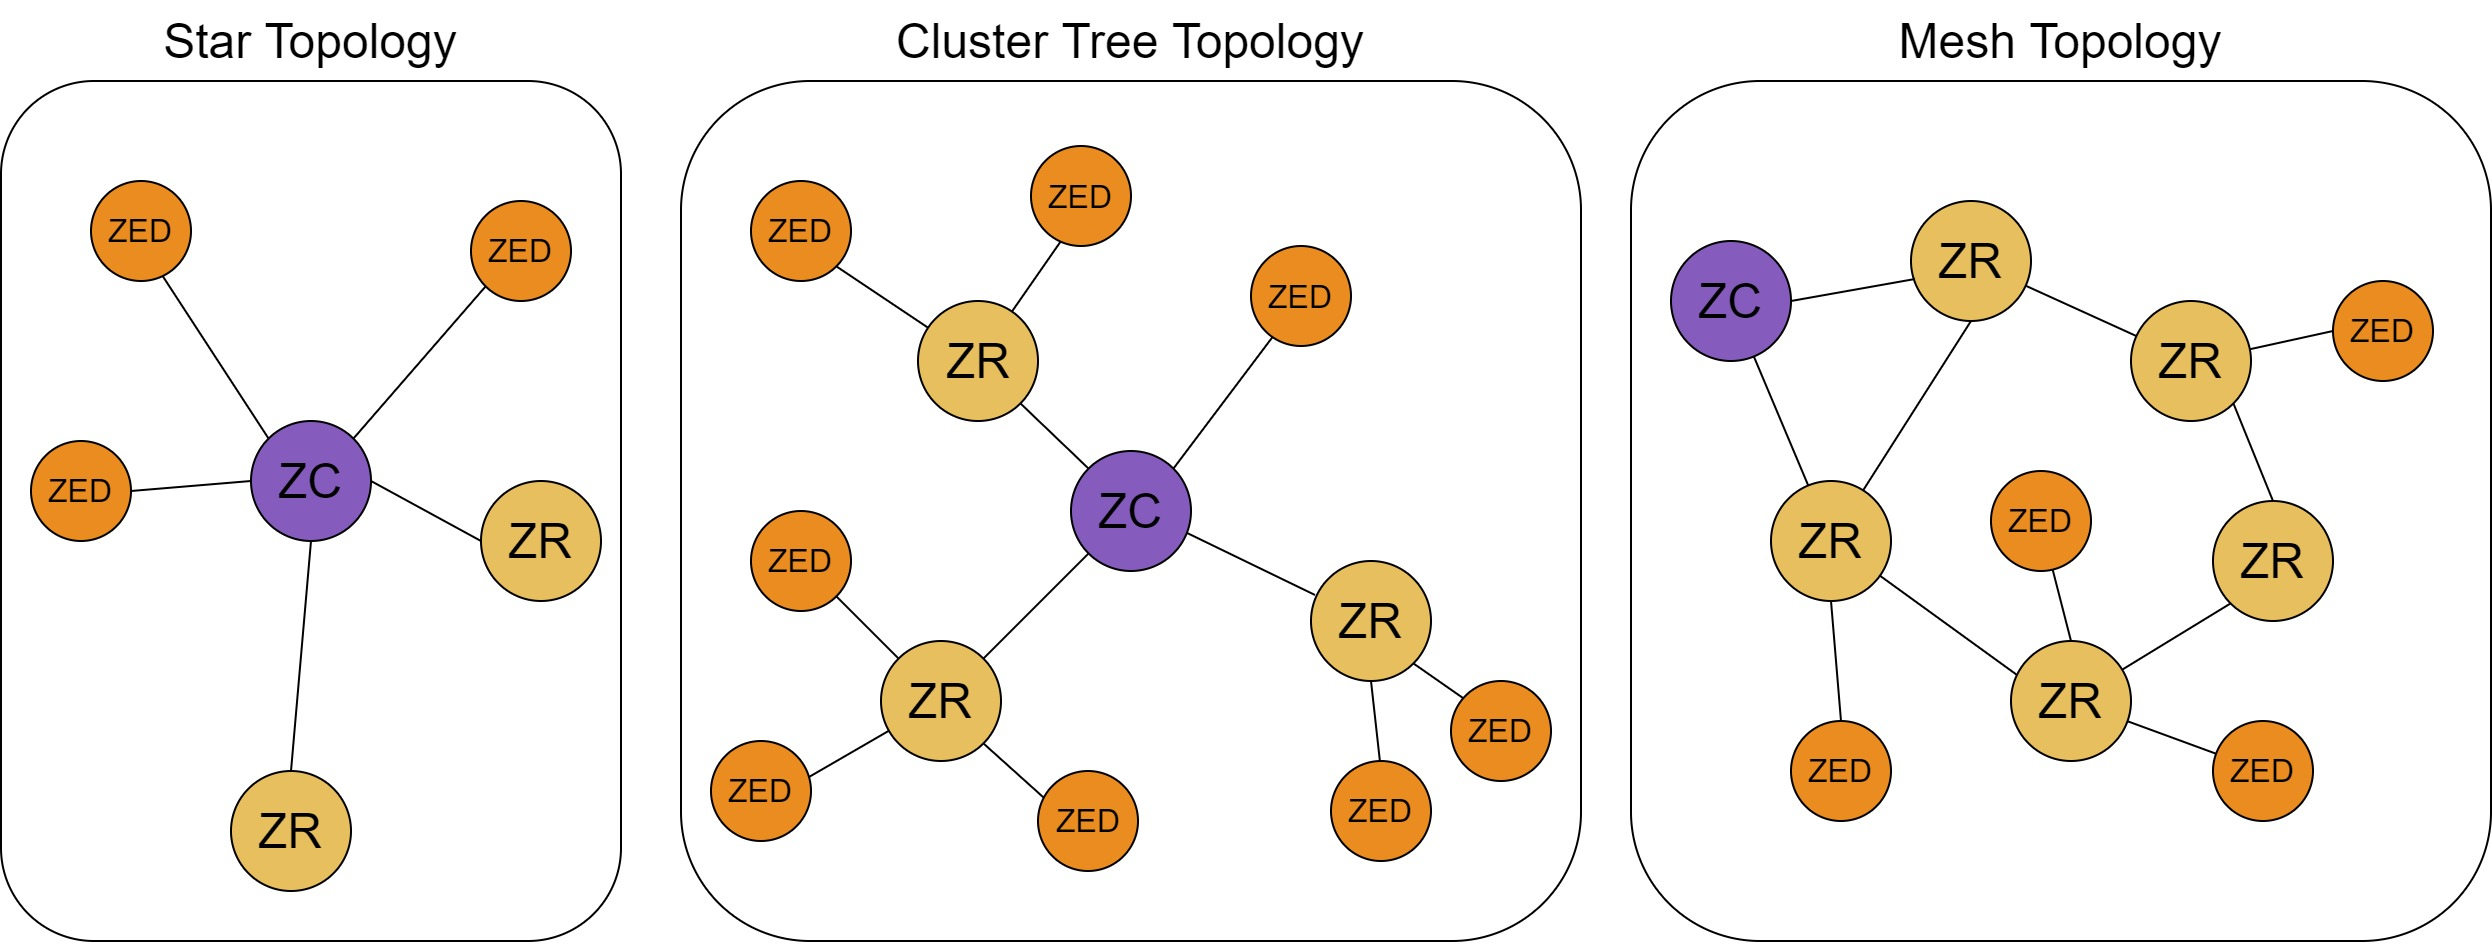
\includegraphics[width=1.0\textwidth]{./images/zigbee-arch.jpg}
  \end{center}
  \vspace{-5pt}
  \caption[Zigbee Netzwerkarchitekturen]{Zigbee Netzwerkarchitekturen}
  \caption*{Quelle: {\cite{IoTAndEdge.2020} (bearbeitet)}}
  \label{fig:zigbee-arch}
  \vspace{-10pt}
\end{figure}

Wie in Abbildung \ref{fig:zigbee-arch} dargestellt, unterstützt das Protokoll Zigbee drei verschiedene Netzwerk-Topologien: Star, Mesh und Cluster-Tree. In allen Topologien ist ein sogenannter \Fachbegriff{Zigbee Coordinator} nötig, der für die Kontrolle des Netzwerks zuständig ist, somit aber gleichzeitig einen Single Point of Failure darstellt, da es stets nur einen Coordinator pro Netzwerk geben kann. Neben dem Coordinator werden außerdem \Fachbegriff{Zigbee Router} benötigt, welche sowohl für das Routing zwischen den Endgeräten, als auch für das Eintreten neuer Endgeräte ins Netzwerk zuständig sind. In der Abbildung werden Coordinator als ZC, Router als ZR und Endgeräte als ZED dargestellt. Mit Zigbee sind Bandbreiten von bis zu 250 Kbits/s möglich, was verglichen zu anderen IoT-Protokollen im höheren Spektrum liegt. Die Reichweite liegt hierbei zwischen 75 und 100 Metern in Gebäuden oder bis zu 300 Metern Luftlinie. Ein Zigbee-Netzwerk ist zwar auf eine maximale Anzahl von 65000 Geräten beschränkt, in der Praxis wird das Limit jedoch bereits weit früher erreicht. Eines der größten Probleme von Zigbee ist der Stromverbrauch. Zwar können Endgeräte in einen Sleep-Modus schalten, um den Verbrauch zu senken, Router und der Coordinator müssen jedoch stets aktiv sein, um das Netzwerk permanent aufrecht zu erhalten. Somit ist es nicht praktikabel, ein Zigbee-Netzwerk über längere Zeiträume batteriebetrieben aufrecht zu erhalten, sofern das ein Anspruch an das Netzwerk sein sollte. Weitere Informationen über ZigBee können in den Artikeln \cite{Rani.2019}, \cite{Salman.2019}  und \cite{ZigBeeSpecification.2015} nachgelesen werden.

\subsubsection{BLE}
\label{sec:ThHi:ble}

Bluetooth ist eine Technologie, die schon seit Jahrzehnten sowohl für den klassischen Datenaustausch, als auch für Zwecke, die wie beispielsweise Audiostreaming eine hohe Bandbreite und große Datenpakete erfordern, genutzt wird. Für Szenarien, in denen ein niedriger Energieverbrauch essentiell wichtig ist, wie zum Beispiel beim Einsatz von batteriebetriebenen Sensoren, ist die Technologie also nicht geeignet. Das ursprünglich 2006 von Nokia entwickelte Protokoll \Fachbegriff{Wibree} ging 2009 in die Bluetooth-Version 4.0 als \Fachbegriff{Bluetooth Low Energy} ein und schafft Abhilfe für das oben genannte Problem. Im Vergleich zum klassischen Bluetooth überzeugt Bluetooth Low Energy, kurz BLE, durch etwa ein Zehntel des Energieverbrauchs und bis zu 15 mal geringeren Latenzen, wobei das Protokoll am besten für kleine Daten\-pakete geeignet ist. 

\begin{figure}[H]
  \vspace{10pt}
  \begin{center}
    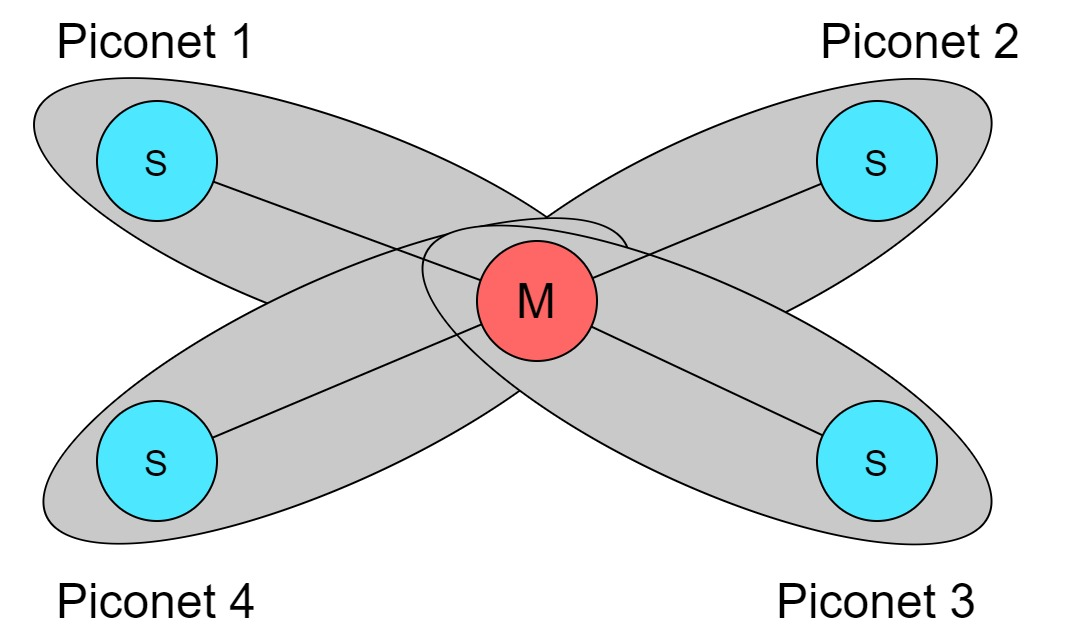
\includegraphics[width=0.6\textwidth]{./images/ble-pico.jpg}
  \end{center}
  \vspace{-5pt}
  \caption[BLE Master-Slave-Architektur]{BLE Master-Slave-Architektur}
  \caption*{Quelle: {\cite{IoTAndEdge.2020} (bearbeitet)}}
  \label{fig:ble-pico}
  \vspace{-10pt}
\end{figure}

Die Netzwerkarchitektur von BLE wird in Abbildung \ref{fig:ble-pico} dargestellt und stellt eine Master-Slave-Architektur dar. Jeder Slave baut hierbei eine Punkt-zu-Punkt-Verbindung zu einem Master auf und bildet ein sogenanntes \Fachbegriff{Piconet}. Mehrere Piconets können außerdem zu einem \Fachbegriff{Scatternet} zusammengeschlossen werden. Master-Nodes sind für die Kontrolle des Netzwerks, das Verbinden von neuen Nodes und die Synchronisation des Netzwerks zuständig. Endgeräte (Slaves) können bei Inaktivität in einen Sleep-Modus wechseln um Energie zu sparen, während Master-Nodes stets aktiv bleiben müssen. Aufgrund des niedrigen Energieverbrauchs und geringen Latenzzeiten wird BLE beispielsweise häufig in Kraftfahrzeugen zur internen Kommunikation von Geräten genutzt. Über Distanzen von etwa 100 Metern können mit Bitraten von bis zu 1 Mbit/s, beziehungsweise 2 Mbit/s bei der Verwendung von Bluetooth 5.0, Daten übertragen werden. Für die Verschlüsselung der Daten wird eine 128-Bit AES-Verschlüsselung genutzt, wobei im Vergleich zu Protokollen wie ZigBee eine eigene Verschlüsselung auf der Anwendungsschicht implementiert werden muss. Technische Details über Bluetooth und BLE können in der offiziellen Bluetooth Specification \Zitat{BluetoothSpecification.2015} gefunden werden, während der Artikel \cite{Salman.2019} einen Vergleich zu anderen Protokollen enthält.

\subsection{Low Power Wide Area Networks}
\label{sec:ThHi:lpwan}

Wie in Kapitel \ref{sec:ThHi:pan} bereits beschrieben wurde, müssen sich IoT-Lösungen, die auf WPAN-Techniken aufbauen, großen Herausforderungen stellen. Zum einen ist der Stromverbrauch der verwendeten Hardware oft sehr hoch, was den Batteriebetrieb von beispielsweise Türsensoren unpraktikabel macht. Zum anderen ist die Reichweite der Funkprotokolle für viele Szenarien mit großen Reichweitenanforderungen wie Smart Cities, oder oft sogar bereits für Smart Buildings nicht ausreichend. Dieser Punkt wird durch das Problem verstärkt, dass Funksignale durch Wände und ähnliche Hindernisse stark abgeschwächt und somit deren Reichweite weiter verringert wird. Für Usecases wie geografisches Tracking sind WPAN-Techniken aufgrund der Reichweite ebenfalls ungeeignet. Aus diesen Gründen steigt seit Jahren die Beliebtheit von LPWAN (Low-power Wide-area-networks) Techniken stark an. Es wird davon ausgegangen, dass im Jahr 2025 über 339 Millionen Geräte durch LPWAN-Techniken vernetzt sein werden \Zitat{Qihao.2019}. Protokolle dieser Klasse zeichnen sich primär durch sehr große Reichweiten aus. Ein nicht zu vernachlässigender Punkt ist außerdem, dass die Datenkommunikation mit sehr geringem Energieverbrauch funktioniert. Durch die hohe Reichweite ist die Bandbreite beim Datenversand geringer als bei WPAN-Techniken, wobei dies bei den normalerweise sehr kleinen IoT-Datenpaketen kein Problem darstellt. Die beliebtesten Netzwerktopologien sind Stern- und Meshtopologien. Meshnetzwerke bieten zwar einige Vorteile wie das Vorhandensein von mehreren Routen zum Nachrichtenversand (Redundanz), was beim Ausfall eines Empfängers Abhilfe schafft, und einfaches Skalieren des Netzwerks ermöglicht, jedoch werden Sterntopologien für LPWANs trotzdem bevorzugt. Dies liegt vor allem daran, dass Meshnetzwerke einerseits teurer sind und andererseits durch redundante Nodes einen deutlich höheren Energieverbrauch als Sterntopologien aufweisen \Zitat{Chaudhari.2020}. In diesem Abschnitt werden die Techniken \Fachbegriff{NB-IoT} und \Fachbegriff{Sigfox} thematisiert. 

\subsubsection{NB-IoT}
\label{sec:ThHi:nbiot}

Das 3rd Generation Partnership Project (3GPP) ist für die Standardisierung von Mobilfunktechniken wie LTE zuständig. Unter diese Standardisierungen fällt auch die 2016 veröffentlichte und für IoT-Zwecke optimierte Technologie \Fachbegriff{Narrowband Internet of Things}, kurz NB-IoT. Die Standardisierung macht es möglich, NB-IoT in das herkömmliche Mobilfunknetz zu integrieren, was einen immensen Vorteil darstellt, da dies die Vision in naher Zukunft ein global nutzbares IoT-Netzwerk zur Verfügung zu haben, sehr realistisch erscheinen lässt. Hier wird der große Vorteil gegenüber WPAN-Techniken klar: es existiert bereits ein Netzwerk, dessen (globale) Abde\-ckung von jedem genutzt werden kann. Dadurch werden Usecases wie Mobilität möglich, was bei WPAN-Technologien unmöglich ist. Eine 200-kHz-Funkzelle kann hierbei mehrere hunderttausend Geräte unterstützen. Der Name ``Narrowband IoT'' ergibt sich daher, dass das Protokoll zwar den LTE-Standard nutzt, sich jedoch auf eine schmale (englisch: narrow) Bandbreite von 200 kHz beschränkt. Zwar sinkt der Datendurchsatz gegenüber LTE, es steigt jedoch die Energieeffizienz und die Reichweite. Mit Geschwindigkeiten von bis zu 250 kb/s bei Downlink und bis zu 20 kb/s Uplink ist die Bandbreite für IoT-Zwecke jedoch weiterhin mehr als ausreichend. Das Nutzen des Mobilfunknetzes bietet immense Vorteile, wobei der größte die Quality of Service ist. Auch Geolokalisierung ist mit NB-IoT über TDoA (Time Difference of Arrival) möglich. Hierbei empfangen mehrere Funkmasten ein Signal gleichzeitig und können anhand der zeitlichen Unterschiede des Eintreffens der Signale den Sender lokalisieren. Das Senden von Daten geschieht über NB-IoT im Vergleich zu anderen LPWAN-Techniken mit hohen Geschwindigkeiten und niedrigen Latenzzeiten, wobei auch das Senden vieler Datenpakete kein Problem darstellt. Da NB-IoT im lizenzierten Spektrum operiert, gibt es hier keine Einschränkung über das Sendeverhalten von Geräten wie bei Protokollen wie Sigfox. Weitere Vorteile sind eine durch den Mobilfunk erprobte Ende-zu-Ende Verschlüsselung und Authentifizierung, hohe Skalierbarkeit, geringe Gerätekosten und eine gute Gebäudedurchdringung der Funksignale. Durch den niedrigen Energieverbrauch können NB-IoT-Geräte jahrelang batteriebetrieben genutzt werden. Dies macht es einfach, selbst komplexe IoT-Netzwerke aufzubauen, da Geräte weder zur Stromversorgung noch zum Datenaustausch verkabelt werden müssen. Jedoch gibt es auch Nachteile bei der Nutzung des Protokolls. Die Nutzung des Mobilfunknetzes ist bei der Nutzung von NB-IoT unabdingbar, es ist also nicht möglich eigene Netzwerke zu erstellen. Sollte beispielsweise die existierende Netz\-abdeckung für ein eigenes Szenario nicht ausreichend, oder ein vollständig privates Netzwerk erwünscht sein, ist NB-IoT für den Anwendungszweck ungeeignet. Außerdem verursacht die Nutzung des lizenzierten Spektrums Kosten, die vom Netzbetreiber festgelegt werden. Während hier nur ein Überblick über das Protokoll gegeben werden soll, beschäftigen sich die Artikel \cite{Aernouts.2018}, \cite{Vodafone.2017} und \cite{Ding.2020} noch detaillierter mit NB-IoT.

\subsubsection{Sigfox}
\label{sec:ThHi:sigfox}

Das französische Unternehmen \Begriff{Sigfox} wurde 2010 von Ludovic Le Moan und Christophe Fourtet mit der Vision gegründet, ein globales LPWA-Netzwerk aufzubauen. Im September 2020 gibt das Unternehmen an, über 16 Millionen Geräte, welche über 41 Millionen Nachrichten pro Tag senden, in 72 Ländern zu vernetzen. Sigfox bietet neben dem proprietären Funkprotokoll eine vollständige Ende-Zu-Ende-Konnektivität, wobei Geräte Daten über das Sigfox-Netzwerk direkt in die Sigfox-Cloud senden \Zitat{Sigfox.2020}. Sigfox operiert in den Frequenzbändern von 868 MHz in Europa, 902 MHz in den USA und 928 MHz in anderen Regionen, welche zum unlizenzierten Spektrum gehören und somit kostenfrei genutzt werden können. Sigfox nutzt in diesem Frequenzband nur 192 kHz und wird deswegen als ``Ultra-Narrow-Band'' bezeichnet. Mit einer Nachrichtenbreite von 100 Hz ist das Sigfox-Protokoll eines der Protokolle mit der schmalsten Bandbreite, wodurch geringe Geschwindigkeiten von bis zu 600 b/s beim Downlink und bis zu 100 b/s beim Uplink entstehen. Hierdurch entstehen im Umkehrschluss außerordentlich große Reichweiten von bis zu 50 Kilometern. Selbst Innenräume können durch das Sigfox-Netzwerk ausreichend abgedeckt werden.\\
Besonders vorteilhaft beim Protokoll Sigfox sind die geringen Kosten. Nutzer zahlen lediglich Sigfox-Nodes und die Kosten für die Nutzung des Netzwerks und der Sigfox-Cloud. Somit ist ein sehr einfaches Setup selbst von großen IoT-Netzwerken möglich, da die Geräteverwaltung und die Speicherung von Daten in einer Cloud ebenfalls Teil der Sigfox-Services ist und nicht selbst aufgesetzt werden muss. Geräte müssen mit Empfängerstationen keine stehende Verbindung halten, wodurch selbst mobile Geräte unterstützt werden. Sigfox-Nodes senden stets ein Paket direkt und zwei Kopien in einer zufälligen Frequenz an Stationen in Reichweite, was die Wahrscheinlichkeit für eine erfolgreiche Übermittlung deutlich erhöht. Die Daten werden hierbei vor dem Versand mit einer AES-Verschlüsselung versehen, um den Datenversand zwischen Gerät und Cloud komplett zu schützen. Die Netzwerktopologie von Sigfox wird als Sterntopologie bezeichnet, da jegliche Kommunikation im Netzwerk über Empfängerstationen (Sterne) des Netzwerks abläuft.\\
Die Nutzung von Sigfox bietet allerdings nicht nur Vorteile. Da Sigfox das gesamte Netzwerk bereitstellt, ist jeder Nutzer an das proprietäre Netzwerk gebunden. Dies ist vor allem deshalb ein Problem, da zum aktuellen Zeitpunkt zwar ein großer Teil Europas, andere Kontinente hingegen kaum durch das Sigfox-Netzwerk abgedeckt sind \Zitat{SigfoxMap.2020}. Somit kann ein Großteil der Welt Sigfox zum aktuellen Zeitpunkt nicht nutzen. Ein weiterer Nachteil ist eher technischer Natur. Sigfox-Nachrichten können lediglich mit 12 Bytes an Daten befüllt werden. Durch binäre Codierung können zwar für viele IoT-Szenarien ausreichend Daten verschickt werden, jedoch ist dies eine enorme Einschränkung gegenüber Protokollen wie NB-IoT. Ein Problem, dem sich alle LPWAN-Protokolle, die im unlizenzierten Spektrum agieren, stellen müssen, sind lokale Regulierungen, sogenannte \Begriff{Duty Cycles}. In Europa ist der Duty Cycle für das unlizenzierte Spektrum 1\%. Dies bedeutet, dass in einer Stunde, 3600 Sekunden, genau 1\% der Zeit gesendet werden darf, was 36 Sekunden entspricht. Da beim Uplink nach einer Nachricht mindestens 6 Sekunden gewartet werden muss, können also pro Gerät sechs Nachrichten pro Stunde, beziehungsweise 140 Nachrichten am Tag als Uplink gesendet werden. Somit ist Sigfox sehr ungeeignet für Szenarien in denen Echtzeitdaten oder eine hohe Nachrichtenanzahl erforderlich sind. Für Szenarien wie Smart Building oder Smart City hingegen ist Sigfox ideal, da die Datenmengen in derartigen Szenarien meist sehr gering und nicht zeitkritisch sind. Neben der offiziellen technischen Übersicht \Zitat{SigfoxTechnical.2017} wird Sigfox in den wissenschaftlichen Artikeln \cite{Aernouts.2018} und \cite{Chaudhari.2020} ausführlich behandelt.


\subsection{Messaging Protokolle}
\label{sec:ThHi:messaging}

Nachdem es Funkprotokolle möglich machen, Daten von Geräten wie Sensoren zu übertragen, müssen die Daten zur Weiterverarbeitung meist in einem System aus Services verbreitet werden. Ein Beispiel für eine solche Verbreitung ist das Hinterlegen eines empfangenen Datensatzes in die richtige Cloudinstanz, abhängig davon, welcher Nutzer hinter dem sendenden Gerät steht. Hierfür existieren diverse Protokolle, die nach dem TCP/IP-Schichtenmodell, anders als die bisher besprochenen Protokolle, der Anwendungsschicht zuzuordnen sind. Da die Anwendungsschicht auf die Netzwerkschicht und die Transportschicht aufbaut, sind derartige Protokolle für die Verbindung IoT-Geräte wie Sensoren zu Empfängern oft ungeeignet, da hierfür ein IP- und TCP-fähiges Netzwerk vorhanden sein muss. Aus diesem Grund werden in diesem Abschnitt kurz zwei Techniken beschrieben und die Frage geklärt, welche davon am besten geeignet ist und warum.

Das wohl älteste Protokoll hierfür ist das \Fachbegriff{Hypertext Transfer Protocol}, kurz HTTP. Das Protokoll baut auf TCP auf und garantiert somit einen erfolgreichen Nachrichtenversand, sowie Stau- und Flusskontrolle. Außerdem ist das Protokoll sehr einfach zu nutzen und auf den meisten Endgeräten implementiert. Trotzdem birgt die Nutzung des Protokolls immense Nachteile. Zum einen nutzt HTTP das Protokoll TCP der Transportschicht des TCP/IP-Modells. Um Nachrichten über TCP senden zu können, muss ein Three-Way-Handshake durchgeführt werden, der bei geringen Nachrichtengrößen, wie es bei IoT typisch der Fall ist, oft aufwendiger ist als das Senden der Daten an sich. Dadurch steigen die benötigten Ressourcen vor allem bei hohem Datendurchsatz stark an. Das Hauptproblem liegt aber in der Natur des HTTP Protokolls selbst. Es wird auf ein Request-Response-Format aufgebaut, was bedeutet, dass ein Sender eine Anfrage stellt und auf eine Antwort warten muss. HTTP wird daher auch als synchrones Protokoll bezeichnet. Dies ist nicht nur zeitaufwendig, sondern erfordert Ressourcen und blockiert eventuell andere Aufgaben. Zuletzt muss erwähnt werden, dass gerade bei der Verbreitung von Daten mit HTTP für jedes Ziel eine eigene Anfrage gestellt werden muss. HTTP scheint also allgemein für diesen Usecase nicht ideal geeignet zu sein \Zitat{Rani.2019}. 

Da das Request-Response-Format offensichtlich für IoT-Systeme eher ungeeignet ist, bauen die meisten modernen Systeme auf Publish-Subscribe-Formate auf. Das für Events optimierte Format besteht aus drei Komponenten: Publisher, Subscriber und Broker. Ein Publisher sendet hierbei Nachrichten an den Broker und versieht die Nachricht mit einer Annotation, dem sogenannten Topic. Subscriber können dem Broker vermitteln, an welchen Nachrichten sie interessiert sind. Hierfür geben die Subscriber ebenfalls ein oder mehrere Topics an. Es ist nun die Aufgabe des Brokers, eingehende Nachrichten an die passenden Subscriber zu verteilen. Hieraus ergeben sich große Vorteile. Zum einen sind Sender und Empfänger zeitlich nicht stark miteinander gekoppelt, es muss also nicht auf eine direkte Antwort gewartet werden. Diese Art von Protokollen kann daher als asynchron beschrieben werden. \\ 
Dies macht derartige Publish-Subscribe-Protokolle gerade für Netzwerke mit großen Latenzzeiten und niedrigen Bandbreiten geeignet, da der Nachrichtenversand keine blockierende Operation darstellt. Zum anderen werden Nachrichten nicht an einen speziellen Empfänger, sondern an eine symbolische Adresse, das Topic, gesendet. Dies macht es gerade in großen Systemen einfach, Nachrichten in einer Viele-zu-Viele-Beziehung zu verbreiten. Zudem ist der Inhalt der Nachrichten nicht an eine Programmiersprache gebunden, da für Sender und Empfänger lediglich das Kommunikationsformat festgelegt werden muss. Meist werden zwar die Formate JSON oder XML genutzt, jedoch kann theoretisch jedes beliebige Format genutzt werden. Das am häufigsten genutzte Protokoll dieser Art ist das \Fachbegriff{Message Queuing Telemetry Transport Protocol}, kurz MQTT. Das leichtgewichtige Protokoll fügt Nachrichten nur einen sehr schmalen Header von 2 Bytes hinzu, was Nachrichten allgemein sehr klein hält. Somit kann eine Vielzahl an Nachrichten verarbeitet werden, ohne die vorhandenen Ressourcen unnötig zu belasten. Neben der einfachen Nutzung des Protokolls existieren Client-Implementierungen für viele Programmiersprachen, was ebenfalls einen großen Vorteil von MQTT ausmacht. Aus diesen Gründen wird MQTT oft als Standard für IoT Messaging bezeichnet (\cite{Happ.2020, Rani.2019}). Weitere sehr beliebte und in vielen Punkten ähnliche Protokolle sind beispielsweise XMPP und AMQP.

\section{LoRa und LoRaWAN}
\label{sec:ThHi:loralorawan}

In diesem Kapitel wird das Protokoll LoRa, mit dem sich die Arbeit hauptsächlich beschäftigt, behandelt. Hierzu wird zunächst auf die Entstehungsgeschichte des Protokolls eingegangen. Daraufhin wird die Frage geklärt, worum es sich bei dem bereits erwähnten \Fachbegriff{LoRaWAN} handelt und welche Verbindung es zu LoRa hat. Ein großer Teil des Kapitels wird sich anschließend mit den technischen Details, der LoRaWAN Netzwerkarchitektur und der Sicherheit des Protokolls beschäftigen. Abschließend wird das ``The Things Network'' und das Unternehmen ``The Things Industries'' und deren Arbeit vorgestellt.

\subsection{Entstehung} 
\label{sec:ThHi:entstehung}

Die Geschichte von LoRa begann im Jahr 2009. Die beiden Franzosen Nicolas Sornin und Olivier Seller gründeten das Unternehmen \Begriff{Cycleo SAS} mit dem Ziel eine Technologie zu entwickeln, die es möglich macht, mit geringem Energieverbrauch Daten über große Distanzen zu übertragen. Hieraus ergibt sich auch der Name \Fachbegriff{LoRa}, welcher lediglich ein Akronym aus den englischen Worten ``Long Range'', also große Reichweite, darstellt. Da es zu dieser Zeit noch kaum vergleichbare Technologien gab, war dieses Protokoll ein revolutionärer Schritt in der IoT-Welt. Der dritte Partner François Sforza trat dem Unternehmen 2010 bei. Die ursprüngliche Zielgruppe von Gas-, Wasser- und Elektrizitätsmessung ähnelte bereits der Art von Vernetzung, die heute als ``Internet of Things'' bekannt ist. Im Mai 2012 kaufte die Firma \Begriff{Semtech} das Unternehmen auf und veröffentlichte das Protokoll \Fachbegriff{LoRaMAC}. Dieses neue Protokoll beinhaltete nicht nur die Datenübertragung durch Funksignale, sondern auch Eigenschaften wie Nachrichtenstandards und Sicherheit. Drei Jahre später, 2015, wurde die \Begriff{LoRa Alliance} gegründet, die bis heute das Ziel verfolgt, ihr Protokoll global nutzbar und Geräte miteinander kompatibel zu machen. Im gleichen Atemzug wurde das Protokoll zu \Fachbegriff{LoRaWAN} umbenannt \Zitat{Slats.2020}. Der Non-Profit-Organisation sind heute über 500 Unternehmen wie beispielsweise IBM und Cisco beigetreten, die alle das gemeinsame Ziel verfolgen, LoRaWAN als Standard für LPWA-Netzwerke nutzbar zu machen. Im November 2020 ist LoRaWAN in 162 Ländern vertreten und zählt somit zu den meist genutzten LPWAN-Technologien \Zitat{LoRaAlliance.2020}.

\subsection{Unterschied zwischen LoRa und LoRaWAN}
\label{sec:ThHi:lorawan}

Wichtig zu verstehen ist der Unterschied zwischen \Fachbegriff{LoRa} und \Fachbegriff{LoRaWAN}. LoRa stellt hierbei die erste, physikalische Schicht des TCP/IP-Schichtenmodells und ist somit lediglich für die Übertragung von Binärdaten zuständig. Für große Lösungen ist LoRa jedoch nicht ausreichend, da wichtige Eigenschaften wie Authentifizierung von Geräten oder eine einheitliche Netzwerkarchitektur nicht vorhanden sind. LoRaWAN ist ein cloudbasiertes Protokoll welches die Netzwerk\-schichten über LoRa abdeckt. Durch LoRaWAN werden, für LPWA-Netzwerke elementar wichtige, Funktionen wie Verschlüsselung und das Filtern duplizierter Nachrichten, bereitgestellt. Auch alle nötigen Netzwerk\-komponenten und deren Struktur werden durch LoRaWAN definiert. Um LoRa also optimal nutzen zu können, wird in beinahe allen Sze\-narien LoRaWAN ebenfalls verwendet. Besonders wichtig ist hierbei, dass LoRa selbst ein proprietäres Protokoll ist, während LoRaWAN ein völliges Open-Source-System darstellt \Zitat{LoRaAlliance.2015}.

\subsection{Technische Details}
\label{sec:ThHi:technisch}

LoRa und das damit verbundene Protokoll LoRaWAN sind in die Klasse der LPWA-Netzwerke in Kapitel \ref{sec:ThHi:lpwan} einzuordnen. Wie bereits erwähnt, stellt LoRa die physikalische Schicht im Netzwerkmodell dar. Protokolle dieser Schicht müssen stets mit Datenkollisionen kämpfen, die genau dann entstehen, wenn mehrere Sender über das gleiche Medium, zum Beispiel ein Ethernet-Kabel, senden. Um derartigen Kollisionen entgegen zu wirken, nutzt LoRa als erstes Protokoll die Modulationstechnik \Fachbegriff{Chirp Spread Spectrum}, kurz CSS, zum Datenversand. Hierbei handelt es sich um eine Technik, welche die Prinzipien mehrerer Modulationstechniken vereint, und somit besonders effektiv ist. Bei diesen Techniken handelt es sich um \Fachbegriff{Amplitude Modulation}, kurz AM, \Fachbegriff{Frequency Modulation}, kurz FM und \Fachbegriff{Phase Modulation}, kurz PM, wobei die ersten beiden Techniken beispielsweise aus dem Radiofunk bekannt sind. Das Ergebnis wird als \Fachbegriff{Multidimensional Multiple Access}, kurz MDMA bezeichnet. MDMA ist somit ausgesprochen robust und löst neben Datenkollisionen viele Probleme, die beim Datenversand mit Funktechniken entstehen können \Zitat{Bastani.2009}. 

Wie auch das in Kapitel \ref{sec:ThHi:sigfox} behandelte Protokoll Sigfox operiert LoRa im unlizenzierten Spektrum und kann somit kostenfrei privat genutzt werden. Die LoRa Alliance definiert diesen Frequenzbereich abhängig von der Region. In Europa wurde dieser beispielsweise auf 863-870 MHz (seltener auch 433-434 MHz) und in den USA auf 902-928 MHz festgelegt. Es gibt jedoch für jede Region eine Standardfrequenz, die beispielsweise für Anfragen zum Beitritt zum Netzwerk genutzt wird, woraufhin der gesamte Frequenzraum zur Verfügung steht. In Europa beträgt diese Frequenz 868 MHz, weshalb die Region auch oft als \Begriff{EU868} beschrieben wird. Ebenfalls ähnlich zu Sigfox existiert für LoRa eine weitere lokale Regulierung, der Duty Cycle. In Europa beträgt dieser meist 1\%, was eine Sendezeit von 36 Sekunden pro Stunde ergibt. Hierbei gibt es jedoch keine maximale Tagesanzahl an Nachrichten wie bei Sigfox, das Limit hängt lediglich von der genutzten Sendezeit und somit von der Sendedistanz und der Datenmenge ab. Da sich auch LoRaWAN-Empfangsstationen, sogenannte Gateways, an diesen Duty Cycle halten müssen, diese jedoch Nachrichten an mehr als nur ein Gerät senden können, wird in der LoRa-Kommunikation die Uplink-Richtung, also von Endgerät zu Gateway, stark präferiert. \\
Aus diesem Grund werden LoRa-Geräte in drei Klassen A, B und C eingeteilt. Jedes Gerät unterstützt hierbei die Klasse A. Diese ist die energiesparendste der Klassen, da sie sich auf Uplink nach der ALOHA-Methode verhält. Dies bedeutet, dass das Gerät Daten dann senden kann, wenn Sendebedarf besteht, und den Rest der Zeit in einem Energiesparmodus verweilen kann. Nach dem Datenversand folgen außerdem zwei kurze Zeitfenster, in welchen das Gerät Daten empfangen kann. Der Energieverbrauch ist hier so gering, dass viele Sensoren über mehrere Jahre rein batteriebetrieben im Einsatz bleiben können. Geräte der Klasse B folgen den Eigenschaften der vorherigen Klasse, jedoch mit dem Zusatz, dass die Geräte in bestimmten Zeitabständen aufwachen, um sich mit dem Netzwerk auszutauschen. Dies bietet den großen Vorteil, dass eine Garantie besteht, dass Daten mit einer bestimmten Verzögerung, die maximal die Aufwachfrequenz des Gerätes ist, an das Endgerät gesendet werden können. Diese Funktionalität macht sich jedoch im Energieverbrauch negativ bemerkbar. Abschließend folgen Geräte der Klasse C. Diese Geräte lauschen stets auf eingehende Nachrichten, sofern das Gerät selbst nicht sendet, weswegen die Geräte auch als halbduplexe Geräte bezeichnet werden können. Da im Gegensatz zu den Klassen A und B auf einen Energiesparmodus verzichtet wird, kostet diese Funktionalität offensichtlich deutlich mehr Energie, was die Geräte ungeeignet für batteriebetriebene Szenarien macht \Zitat{LoRaAlliance.2015}. 

Ein Aspekt, der LoRa stark von Sigfox unterscheidet, ist die Aufteilung des Frequenzraums in Kanäle. In Kombination mit der Nutzung des Chirp Spread Spectrums können somit Nachrichten gleichzeitig auf verschiedenen Kanälen gesendet werden, ohne Kollisionen zu verursachen \Zitat{LoRaAllianceRegional.2020}. In Europa beispielsweise definiert LoRaWAN 10 Kanäle mit einer variablen Datenrate von 250 b/s bis 5.5 kb/s, einen Kanal für schnelle Übertragungen mit bis zu 11 kb/s und einen FSK Kanal mit 50 kb/s, was die technisch höchste Datenrate von LoRaWAN darstellt \Zitat{LoRaAlliance.2015}. FSK steht hierbei für Frequency Shift Keying, worauf in dieser Arbeit jedoch nicht weiter eingegangen werden soll. Es gilt hier zu beachten, dass verschiedene Kanäle unterschiedliche Bandbreiten nutzen.

Zur Berechnung des tatsächlichen Datendurchsatzes müssen zwei weitere Konzepte verstanden werden. Zum einen ist das die sogenannte Coding Rate. Diese gibt an, wie groß der Teil eines LoRa-Pakets ist, der Daten beinhaltet, wobei der Rest des Pakets Metainformationen und ähnliches beinhaltet. Zum anderen kommt einer der wichtigsten Aspekte des LoRaWAN-Nachrichtenversands ins Spiel: der Spreading Factor, abgekürzt SF. Der Spreading Factor reicht von 7 bis 12, kann also 6 Werte annehmen. Je niedriger der Spreading Factor, desto höher die Datenrate. Es gilt jedoch zu beachten, dass sich die Sendereichweite indirekt proportional zum Spreading Factor verhält, also mit höherer Datenrate nur über geringere Reichweiten gesendet werden kann. Die SF-Auswahl hängt daher von der Entfernung zur Empfangsstation ab: befindet sich ein Endgerät nah am Empfänger, wird ein möglichst geringer SF gewählt, um durch das schnelle Senden der Nachricht mit einer hohen Datenrate das Netz nur einer möglichst geringen Belastung auszusetzen. Außerdem ist es durch verschiedene Spreading Factors ebenfalls möglich gleichzeitig Daten ohne Interferenzen zu senden, was gerade bei vielen verschiedenen Netzwerken in Kombination mit den anderen Modulationstechniken zu einem sehr robusten Sendeverhalten führt. 

Wie bei allen Funktechnologien ist es schwer, eine allgemeine Aussage über die tatsächliche maximale Sendereichweite, also mit dem höchsten Spreading Factor und der geringsten Datenrate, zu treffen. Viele Tests ergeben jedoch Distanzen von 2-5 Kilometern in städtischen Regionen und bis zu 30 Kilometern bei einer direkten Übertragung ohne Hindernisse \Zitat{Ertuerk.2019}. Somit ist es möglich mit wenigen Empfängerstationen ganze Städte abzudecken oder in Usecases wie Smart Buildings mit nur einem Gateway selbst Geräte in großen Gebäuden zu vernetzen.\\
Auch LoRaWAN ermöglicht es, einen Sender über den Zeitunterschied oder den Unterschied der Stärke der Signaleingänge zu orten, sollte das Signal von mehreren Empfangs\-stationen des gleichen Netzwerks empfangen werden. Durch die hohe Reichweite können also auch mobile Usecases verwirklicht werden.

Der wohl größte Vorteil gegenüber anderen LPWAN-Techniken, speziell der sehr ähnlichen Technologie Sigfox, ist die Möglichkeit eigene Netzwerke aufbauen zu können. Zwar ist die Anzahl der Nachrichten ähnlich wie bei Sigfox durch einen Duty Cycle limitiert, jedoch wird die maximale Nachrichtenanzahl nur durch die Uplink-Zeit, nicht aber durch Sendepausen wie bei Sigfox beeinflusst. Da LoRa im unlizen\-zierten Spektrum operiert, fallen für die Nutzung des Funkspektrums keinerlei Kosten an. Um ein eigenes Netzwerk aufzubauen, werden als Hardware lediglich ein LoRa-Gateway als Empfangsstation und LoRa-Endgeräte benötigt. Im Jahr 2020 existiert hierfür ein großer Markt, wodurch LoRa eine der günstigsten Techniken für ein eigenes LPWA-Netzwerk darstellt. Wie im Kapitel \ref{sec:ThHi:architektur} näher erläutert wird, können die Kosten für ein Gateway sogar vernachlässigt werden, wenn das Netzwerk eines externen Providers anstelle eines eigenen Netzwerks genutzt wird. Auch glo\-bale öffentliche Netzwerke sind mit LoRaWAN möglich, wobei eines davon in Kapitel \ref{sec:ThHi:ttntti} behandelt wird.


\subsection{LoRaWAN Netzwerkarchitektur} % Sicherheit nur kurz erwähnen, dann im nächsten Punkt
\label{sec:ThHi:architektur}

Die Softwareseite eines LoRaWAN-Netzwerks hingegen folgt im internen Aufbau der modernen Service-orientierten Architektur, kurz SOA. Im Gegensatz zu bis\-herigen Ansätzen werden Softwarefunktionalitäten in Services gruppiert und somit die mono\-lithische Applikation in mehrere kleine Applikationen aufgeteilt. Neben den typischen Vorteilen von SOAs gegenüber Monolithen bietet diese Struktur hier vor allem zwei große Vorteile. Wie im Kapitel \ref{sec:ThHi:sicherheit} weiter erklärt wird, werden Nachrichten, die durch den LoRaWAN-Stack gesendet werden, mehrfach verschlüsselt. Da es lediglich einen Service gibt, der sich mit dieser Verschlüsselung beschäftigt, senden die anderen Services (selbst das Gateway) die Daten lediglich weiter, ohne sie lesen zu können. Somit kann Vertrauen zu externen Netzwerkprovidern aufgebaut werden. Außerdem können die einzelnen Komponenten auf verschiedenen Geräten bereitgestellt werden. Dies dient nicht nur der Lastverteilung sondern gehört teilweise zur Funktionalität des LoRaWAN-Stacks. So wird beispielsweise der Service \Fachbegriff{Packet Forwarder} immer auf den LoRaWAN-Empfangsstationen, sogenannte Gateways, installiert.

Die Softwarekomponenten eines LoRaWAN-Netzwerkes sind der \Begriff{Packet Forwarder}, die \Begriff{Gateway Bridge}, der \Begriff{Join Server}, der \Begriff{Network Server} und der \Begriff{Application Server}. Auf die Aufgaben jeder Komponente wird nun intensiv eingegangen. Es gilt hier zu erwähnen, dass dies die typische LoRaWAN-Netzwerkarchitektur darstellt, und durchaus Abwandlungen dieses Aufbaus existieren. 

\begin{figure}[H]
  \vspace{10pt}
  \begin{center}
    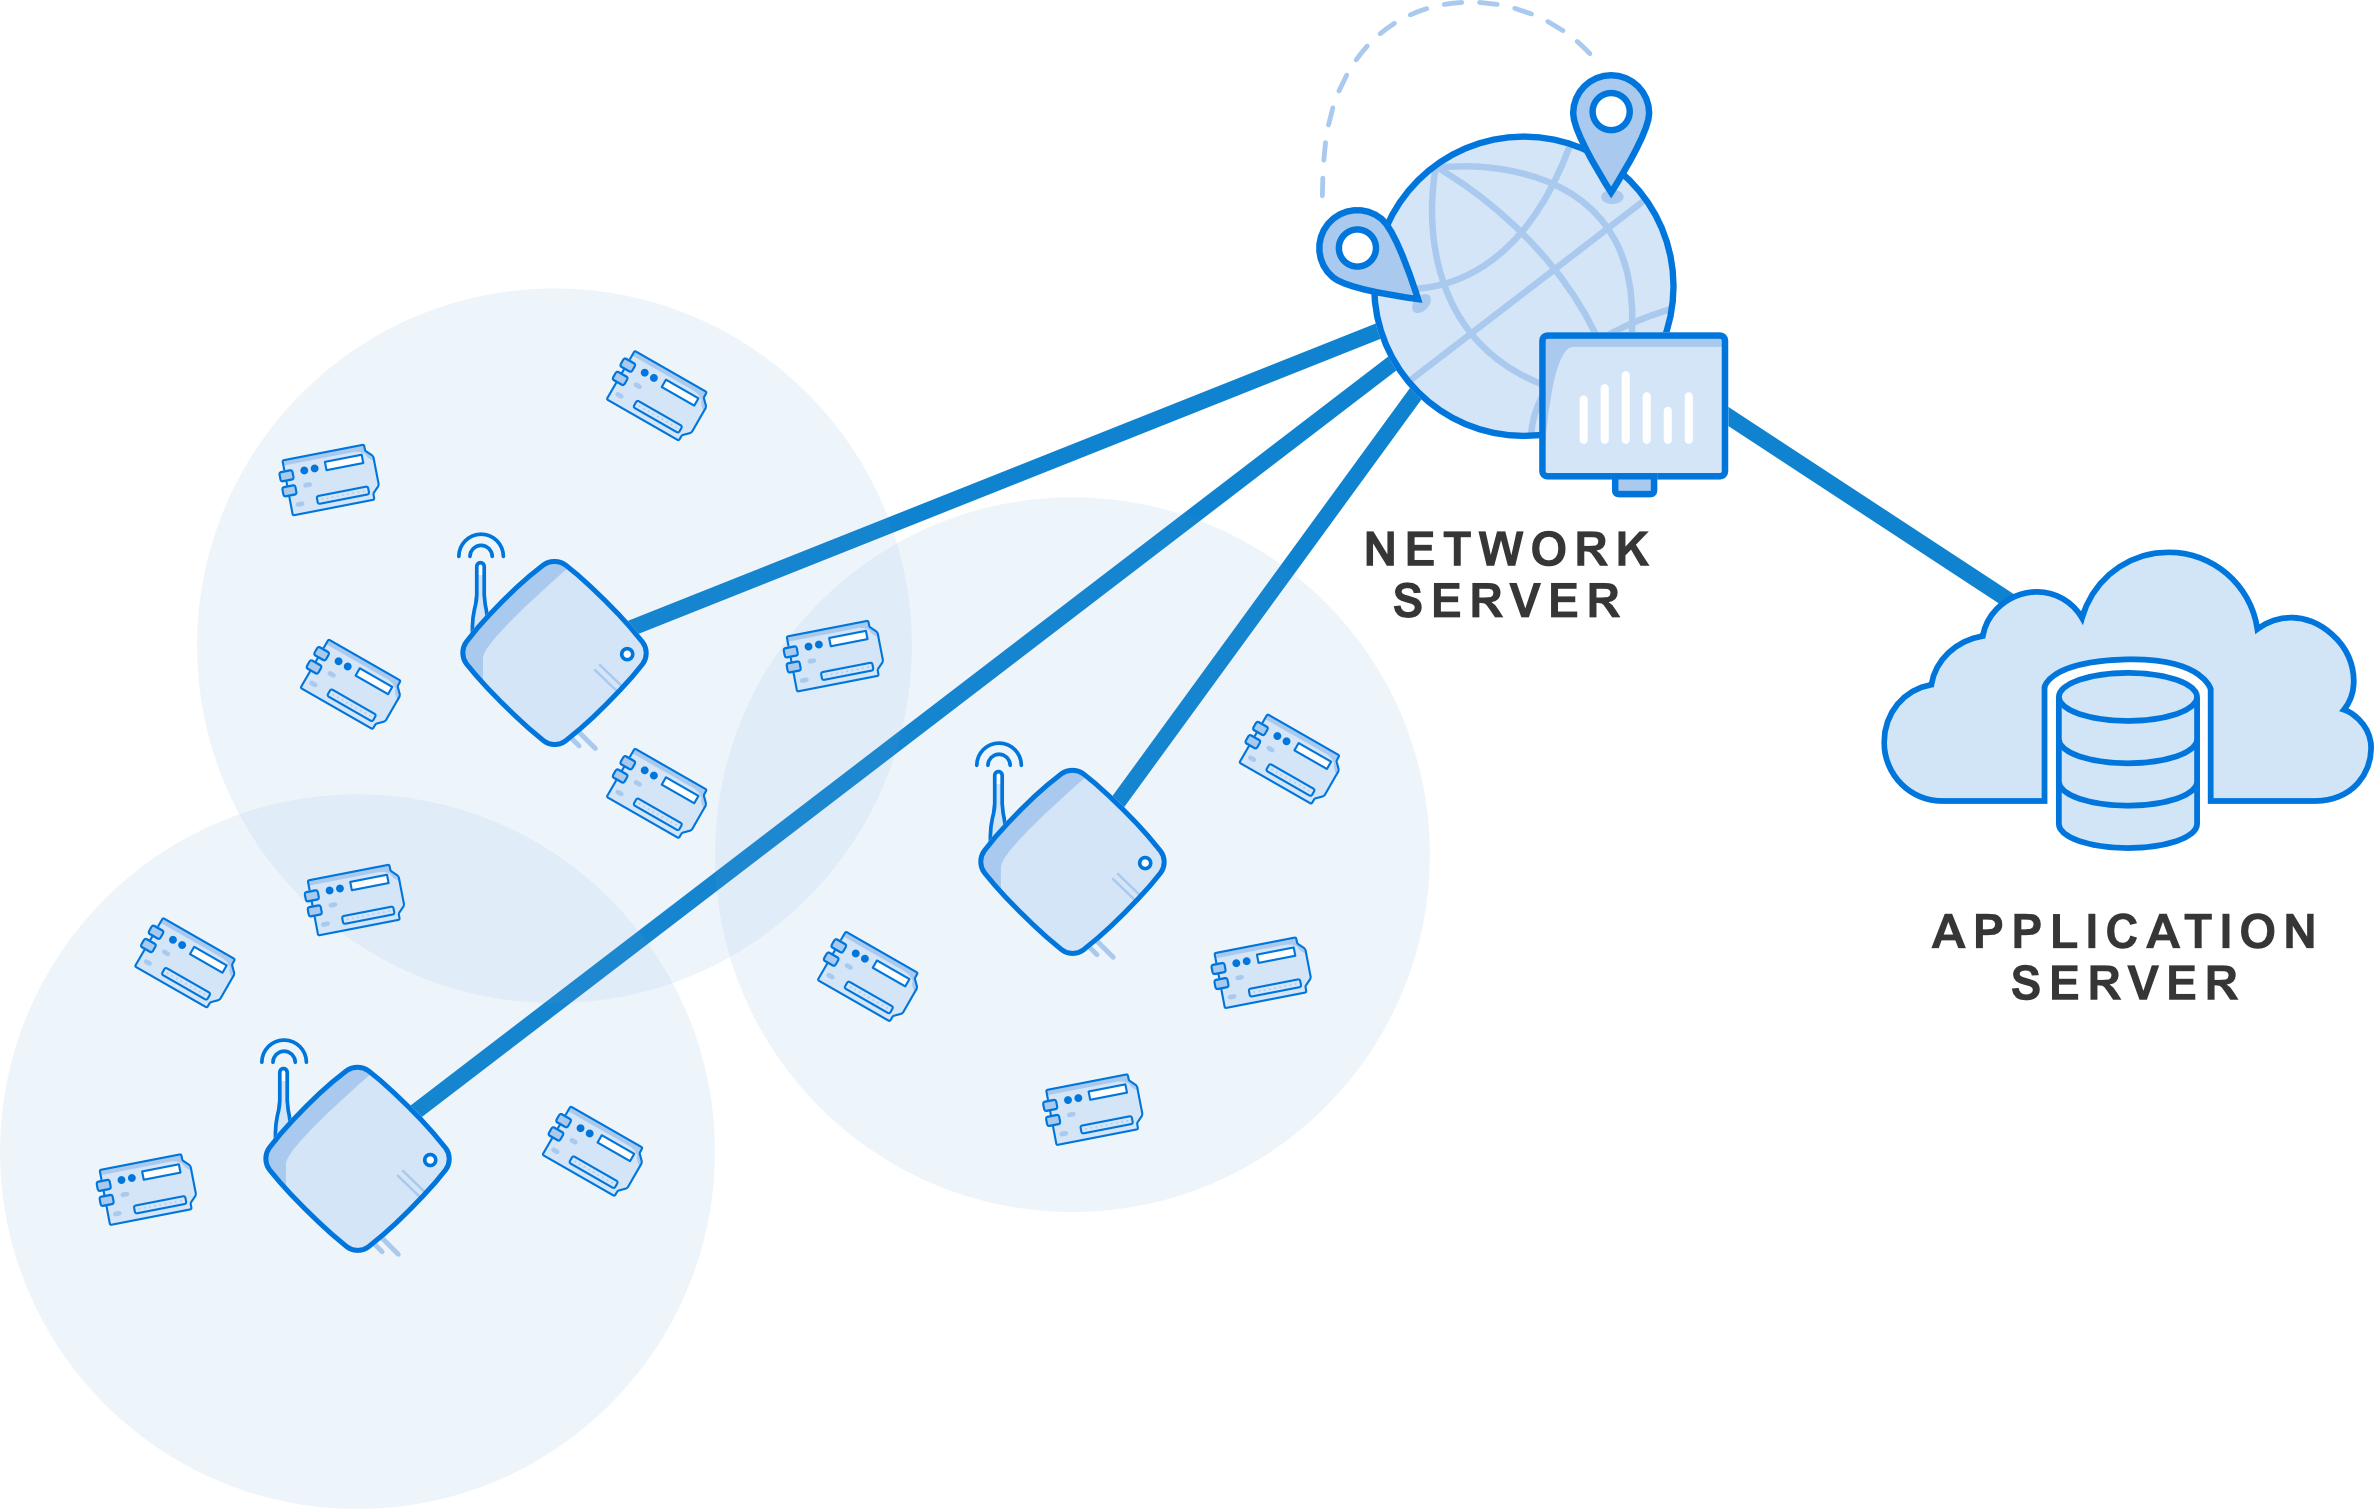
\includegraphics[width=0.7\textwidth]{./images/ttn-arch-star.jpg}
  \end{center}
  \vspace{-5pt}
  \caption[LoRaWAN Star-of-Stars-Topologie]{LoRaWAN Star-of-Stars-Topologie}
  \caption*{Quelle: {thethingsnetwork.org/docs/network/architecture.html}}
  \label{fig:ttn-arch-star}
  \vspace{-10pt}
\end{figure}

Wie aus Abbildung \ref{fig:ttn-arch-star} hervorgeht, stellt ein LoRaWAN-Netzwerk eine Star-of-Stars-Topologie dar, wobei der Network Server das Zentrum beziehungsweise der zentrale Stern der Topologie ist. Gateways stellen im Netzwerk die kleineren Sterne dar und leiten Nachrichten lediglich von den Endgeräten zum Network Server weiter. Außerdem wird hier der Begriff LoRaWAN statt LoRa verwendet, da es sich hier um die gesamte Netzwerkarchitektur und nicht nur um das Protokoll zum Datenversand vom Endgerät zum Empfänger handelt.

Wird ein Signal von einem LoRaWAN-Endgerät gesendet, wird dieses Signal als erstes von einem LoRaWAN-Gateway empfangen. Das Gateway hat eine der wichtigsten Aufgaben im Netzwerk: es dient als Proxy vom Endgerät in den LoRaWAN-Stack, welcher meist in cloudbasierten Lösungen lebt. Diese Funktionalität der Weiterleitung übernimmt der sogenannte Packet Forwarder. Dieser erfüllt also die relativ einfache Aufgabe, Nachrichten über LoRa zu empfangen und über ein IP-basiertes Protokoll, häufig UDP, weiter zu leiten.\\ Die meisten Gateways nutzen hierfür den von Semtech entwickelten \Fachbegriff{Semtech UDP Packet Forwarder}. Die Komponente ist die Minimalanforderung an installierter Software auf einem Gateway. Die verbleibenden Komponenten können theoretisch alle in der Cloud bereitgestellt werden. Per UDP werden die empfangenen Daten an die nächste Softwarekomponente, die Gateway Bridge, weitergeleitet.
Die Gateway Bridge hat die Aufgabe, das Format des Packet Forwarders in ein für den LoRaWAN-Stack normiertes Datenformat umzuwandeln, und die umgewandelten Daten weiterzuleiten. Hierbei sind die beliebtesten Formate \Fachbegriff{JSON} und Googles \Fachbegriff{Protobuf}. Weitergeleitet werden die Daten im neuen Format an einen Message Broker über ein Messaging Protokoll (siehe Kapitel \ref{sec:ThHi:messaging}) wie zum Beispiel MQTT. Die gesamte folgende netzwerkinterne Kommunikation geschieht also asynchron. Der Grund hierfür ist die Entlastung der einzelnen Komponenten: müsste die Gateway Bridge auf den erfolgreichen Versand und deren Antwort warten, und währenddessen blockieren, könnten andere Nachrichten verloren gehen. Somit können selbst Ausfälle einzelner Komponenten toleriert werden, da der Message Broker Daten zwischenspeichert und auch verspätet ausliefern kann.\\
Die Gateway Bridge kann entweder direkt auf dem Gateway oder mit den anderen Komponenten auf einem Server beispielsweise in der Cloud bereitgestellt werden. Für die Installation auf dem Gateway selbst spricht, dass MQTT über TCP läuft, und daher einen erfolgreichen Nachrichtenversand garantiert, während der Packet Forwarder UDP nutzt, welches verlorengegangene Nachrichten schlicht ignoriert. Außerdem ist es mit UDP nicht möglich eine verpflichtende Authentifizierung durchzuführen, da jeder das UDP Paket eines fremden Senders nachahmen und sich somit als dieser ausgeben kann. Mit MQTT besteht die Möglichkeit einer Authentifizierung, weswegen MQTT präferiert werden sollte. Meist wird die Gateway Bridge mit den verbleibenden Komponenten installiert, um sowohl Gateways mit, als auch Gateways ohne installierte Gateway Bridge unterstützen zu können. \\
Folgt man weiter dem Datenfluss, erreicht man nun den Network Server, das Herz der LoRaWAN Sterntopologie. Dieser bearbeitet nicht nur die meisten Aufgaben sondern ist für den Großteil der LoRaWAN-Funktionalität zuständig. Beachtet man vorerst nur den Datenfluss, ist die Hauptaufgabe des Network Servers Daten zwischen Gateways und der nächsten Komponente, dem Application Server, auszutauschen. Wurden die von den Endgeräten versendeten Daten von mehreren Gateways empfangen, ist es außerdem die Aufgabe des Network Servers, diese Duplikate zu erkennen und zu filtern. Hierbei werden Daten nicht direkt an den Network Server gesendet, da die vorherige Komponente, die Gateway Bridge, die Nachrichten bereits auf einem Message Broker hinterlegt hat. Wie in Kapitel \ref{sec:ThHi:messaging} erklärt, muss sich der Network Server also lediglich auf das passende Topic subscriben um die Nachrichten zu erhalten. \\
Die Aufgaben der Komponente betreffen aber nicht nur den Datenversand, sondern das gesamte Netz. Der Network Server ist beispielsweise für die Behandlung von Join Requests/Responses, also dem Beitritt neuer Geräte ins Netzwerk zuständig. Diese Verarbeitung solcher Requests und die Verschlüsselung der Nachrichten werden jedoch nicht vom Network Server selbst erledigt, sondern an den sogenannten \Fachbegriff{Join Server} delegiert. Außerdem steuert der Network Server die sogenannte \Fachbegriff{Adaptive Data Rate}, kurz ADR. Somit wird die Data Rate aller Geräte gesteuert, um beispielsweise Netzwerküberlastung zu vermeiden, beziehungsweise zu behandeln. Hat der Network Server beim Datenempfang all seine Arbeit geleistet, sendet er die verarbeiteten Daten wieder zum Message Broker. \\
Die letzte Komponente, die sich direkt mit dem Datenfluss beschäftigt, ist der Application Server. Auch diese Komponente ist für wichtige Aufgaben zuständig. Hierfür gilt es zu verstehen, dass der Application Server das Administrationswerkzeug eines LoRaWAN-Netzwerks darstellt. Über eine Weboberfläche kann das Netzwerk selbst verwaltet werden, also zum Beispiel neue Endgeräte oder Gateways registriert werden. Wird ein externer Netzwerkprovider genutzt, ist dies besonders wichtig, da nur durch diese Registrierung Daten vom Network Server an die richtige Adresse gelangen. Derartige Server bieten meist eine komfortable Nutzerverwaltung, um gemeinsam auf das eigene Netzwerk zugreifen zu können. Außerdem können zusammengehörige Endgeräte in Gruppen, sogenannte Applications, eingeteilt werden. Da über LoRaWAN versendete Daten meist binär enkodiert werden, um das Netzwerk durch geringere Datenmengen weniger zu belasten und selbst mehr Sendeflexibilität zu erreichen, bietet der Application Server die Möglichkeit, die Nachrichten beim Empfang mit sogenannten Decoder-Funktionen zu decodieren. Meist werden diese Funktionen vom Gerätehersteller mitgeliefert, diese können jedoch nach Belieben verändert oder sogar komplett selbst geschrieben werden. 

\begin{figure}[H]
  \vspace{10pt}
  \begin{center}
    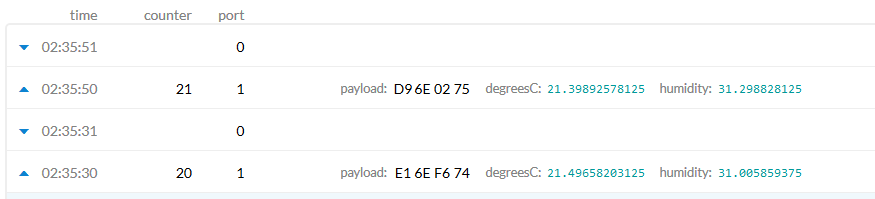
\includegraphics[width=1.0\textwidth]{./images/payload-decoding.png}
  \end{center}
  \vspace{-5pt}
  \caption[Payload Dekodierung]{Payload Dekodierung}
  \caption*{Quelle: {learn.adafruit.com/the-things-network-for-feather/payload-decoding}}
  \label{fig:payload-decoding}
  \vspace{-10pt}
\end{figure}

In Abbildung \ref{fig:payload-decoding} kann erkannt werden, wie aus einem binären Payload in hexadezimaler Schreibweise durch eine hinterlegte Decoder-Funktion ein Temperatur- und ein Luftfeuchtigkeitswert ausgelesen werden.

Neben der Organisation des Netzwerks wird der Application Server außerdem als API für IoT-Usecases wie beispielsweise der Datenvisualisierung genutzt. Hierfür bietet der Application Server APIs über Protokolle wie MQTT an, über die externe Clients die Daten selbst beziehen können. Auch sogenannte Integrations sind eine beliebte Möglichkeit, Daten weiterzuverarbeiten. Mit Integrations können empfangene Daten direkt vom Application Server weiterverarbeitet werden. Die InfluxDB-Integration, welche von vielen Application Servers implementiert wird, kann beispielsweise Messwerte direkt in eine Datenbank schreiben. \\
Über den Application Server können auch Daten an Endgeräte gesendet werden, was oft aus Konfigurations\-zwecken notwendig ist, da bei vielen Geräten keine Möglichkeit besteht, direkt auf die Software zuzugreifen, um diese zu konfigurieren.
Für die Netzwerksicherheit ist der bereits erwähnte Join Server zuständig. Je nach Implementierung ist dieser entweder wie beim \Fachbegriff{The Things Network} als separater Service bereitgestellt oder wie beim \Fachbegriff{ChirpStack} in einer Komponente, in diesem Fall im Application Server, integriert. Wichtig hierbei ist, dass der Network Server keine Kontrolle über die Verschlüsselung hat und somit der Betreiber des Netzwerks keinerlei fremde Nachrichten lesen kann. Auf die Funktionsweise der Verschlüsselung wird im Kapitel \ref{sec:ThHi:sicherheit} näher eingegangen. Bei der Recherche für dieses Kapitel wurden die Quellen \cite{TTNArch.2020}, \cite{ChirpArch.2020} und \cite{TTSApp.2020} hinzugezogen.


\subsection{Sicherheit}
\label{sec:ThHi:sicherheit}

LoRaWAN legt einen sehr hohen Wert auf die Sicherheit des Nachrichtenversands und nutzt eine 128-bit AES-Verschlüsselung. Jedes Endgerät wird vom Hersteller mit drei Keys ausgeliefert. Diese Keys sind eine \Fachbegriff{64-Bit-DevEUI}, eine \Fachbegriff{64-Bit-AppEUI} und ein \Fachbegriff{128-Bit-AppKey}, wobei EUI jeweils für Extended Unique Identifier steht. Diese Keys werden dann benötigt, wenn ein Gerät versucht, dem Netzwerk beizutreten. Beim erfolgreichen Netzwerkbeitritt werden zwei 128-bit Schlüssel generiert, der \Fachbegriff{NwkSKey} (Network Session Key) und der \Fachbegriff{AppSKey} (Application Session Key), wobei beide Schlüssel für nur dieses Gerät und diese Session genutzt werden. Verlässt ein Gerät das Netzwerk und tritt erneut bei, werden also zwei neue Schlüssel generiert. Wie später näher beschrieben wird, weicht dies jedoch bei der Aktivierungsmethode ``Activation by personalization'' ab. Sobald die Geräte beigetreten sind, werden alle Nachrichten zwischen dem Netzwerk und dem neuen Gerät mithilfe dieser beiden Schlüssel verschlüsselt. Der NwkSKey wird nach der Generierung zwischen dem Endgerät und dem Network Server geteilt und ist für deren sichere Kommunikation zuständig. Außerdem ist es durch den Schlüssel möglich, Nachrichten über eine Prüfsumme zu validieren, beziehungsweise Veränderungen festzustellen. Der AppSKey hingegen wird nur zwischen dem Endgerät und dem Application Server ausgetauscht. Dieser Key erlaubt es, Nachrichten Ende-zu-Ende zu verschlüsseln und zu versenden, sodass Komponenten wie der Network Server den Inhalt der Nachrichten nicht verstehen können. Dies ist besonders dann wichtig, wenn ein externer Netzwerkanbieter statt eines privaten Netzwerks genutzt wird, da hierdurch für diesen keine Möglichkeit besteht, Daten, die über sein Netzwerk versendet werden, zu lesen. Wie man also sieht, bietet LoRaWAN sowohl Sicherheitsvorkehrungen auf der Netzwerk-, als auch auf der Anwendungsebene.

Wie funktioniert jedoch der Beitritt zum Netzwerk? Allgemein werden neue Geräte vorerst im Application Server registriert, denn erst wenn das Gerät registriert ist, kann eine Join Request, also eine Anfrage, dem Netzwerk beizutreten, gestellt werden. Bei der Registrierung werden die bereits erwähnten Schlüssel des Endgeräts, nämlich die global eindeutige DevEUI, die AppEUI und der AppKey hinterlegt und außerdem die Aktivierungsmethode gewählt. Hierfür gibt es zwei verschie\-dene Methoden: \Fachbegriff{Over-The-Air-Activation (OTAA)} und \Fachbegriff{Activation-By-Personalization (ABP)}. OTAA stellt die Standardaktivierungsmethode für Endgeräte dar und ist die sicherere der beiden Methoden. Hier sendet ein Endgerät eine Join Request bestehend aus 4 Werten an den Network Server. Diese Werte sind die DevEUI, die AppEUI, die DevNonce und der Message Integrity Code, kurz MIC. Die DevNonce stellt hierbei eine zufällig generierte Zahl dar, die vor Angriffen auf den Aktivierungsprozess schützen soll. Der MIC wird für die Validierung der Nachricht wie auch beim späteren Nachrichtenversand genutzt. Wie oben erwähnt, werden bei einer validen Join Request nun der NwkSKey und der AppSKey mithilfe der Daten in der Join Request generiert. Der Network Server antwortet in einer Join Response mit einigen Werten, wobei der wichtigste die DevAddr ist. Die DevAddr ist eine netzwerkinterne, eindeutige Adresse, die für das neue Endgerät generiert wurde. Von nun an können das Endgerät und der Network Server verschlüsselt kommunizieren. Bei der alternativen ABP-Methode sind die DevAddr, der NwkSKey und der AppSKey bereits an das Gerät gebunden, es müssen also keine Schlüssel oder andere Werte generiert werden. Daher kann ein Netzwerkbeitritt ohne Join-Prozedur ablaufen. Der große Unterschied zwischen den Methoden ist daher, dass OTAA Keys, welche die gesamte Verschlüsselung von LoRaWAN steuern, für jede Session, also jede Registrierung eines Geräts neu generiert, während sich Keys bei ABP ohne manuelles Überschreiben nie ändern. Somit bietet ABP mehr Angriffsmöglichkeiten als OTAA und wird daher seltener verwendet. Zusammenfassend lässt sich sagen, dass LoRaWAN die bereits sehr umfangreiche Netzwerksicherheit auf bewährten Techniken wie AES aufbaut und auch weiterhin die Sicherheit eines LoRaWAN-Netzes durch regel\-mäßige Updates verbessert wird. Die Informationen dieses Kapitels stammen aus den Artikeln \cite{TTNSec.2020} und \cite{SmartMakers.2018}.


\subsection{The Things Network und The Things Industries}
\label{sec:ThHi:ttntti}

In dieser Arbeit wurden bereits mehrfach externe Netzwerkprovider erwähnt. Beschäftigt man sich mit LoRa und LoRaWAN, so stößt man früher oder später auf die Begriffe ``The Things Network'' und ``The Things Industries''. In diesem Kapitel wird erläutert, worum es sich bei den Begriffen handelt und wofür diese nützlich sind.

Bei dem The Things Network, kurz TTN, handelt es sich um ein völlig öffentliches LoRaWAN-Netzwerk. Unter öffentlich versteht man hierbei, dass es jedem möglich ist, Nachrichten über ebenfalls öffentliche Gateways zu senden. Zwar können mit eigenen Gateways und weiterer Hardware eigene ``The Things Network''-Netzwerke aufgebaut werden, da das TTN vollständig Open Source ist, jedoch ist es erwünscht, dem existierenden, kollaborativen Netzwerk beizutreten und dieses somit immer weiter zu vergrößern. Hierbei gilt es zu erwähnen, dass das The Things Network Forum aufgrund der riesigen Community eine der besten Ressourcen für LoRaWAN ist, in der viele Experten ihre Erfahrungen teilen oder auf Fragen antworten. Durch die große Community steigt jedoch nicht nur der Wissensaustausch, sondern auch die Netzwerkgröße. Die mittlerweile fast 16 000 Gateways in 150 Ländern im öffentlichen Netzwerk leiten LoRa-Nachrichten an den cloudbasierten Network Server weiter. Über die TTN-Console, welche ein User Interface zum, ebenfalls cloud\-basierten, Application Server darstellt, können Gateways und Endgeräte ins Netzwerk aufgenommen werden. Auch die anderen in Kapitel \ref{sec:ThHi:architektur} genannten Komponenten sind im The Things Network meist in der Cloud vertreten, wobei der gesamte Softwarestack auch als ``The Things Stack'' bezeichnet wird. Die einzige neue Komponente ist der \Fachbegriff{Identity Server}, der für die Zuordnung von Ressourcen im Netzwerk zu Nutzern und deren Verwaltung zuständig ist. Eine weitere Neuheit ist das \Fachbegriff{Gateway Connector Protocol}. Das Protokoll ersetzt das UDP-Protokoll in der Kommunikation zwischen Gateway und Network Server und löst wichtige Probleme wie den Mangel einer Authentifizierung oder einer Verschlüsselung die Veränderung der gesendeten Daten erkennt und behebt. Mit diesem Protokoll können Daten dann entweder per gRPC oder MQTT an den Network Server gesendet werden \Zitat{TTNGwConn.2020}.

Denkt man über ein öffentliches LoRaWAN-Netzwerk nach, werden schnell viele Vorteile klar. Ist ein Nutzer in Reichweite eines der öffentlichen Gateways, ist es ihm mit dem TTN möglich, LoRa-Geräte zu registrieren und zu nutzen, ohne selbst ein Gateway einrichten zu müssen. Existierende Gateways können hierbei über eine Karte eingesehen werden. 

\begin{figure}[H]
  \begin{center}
    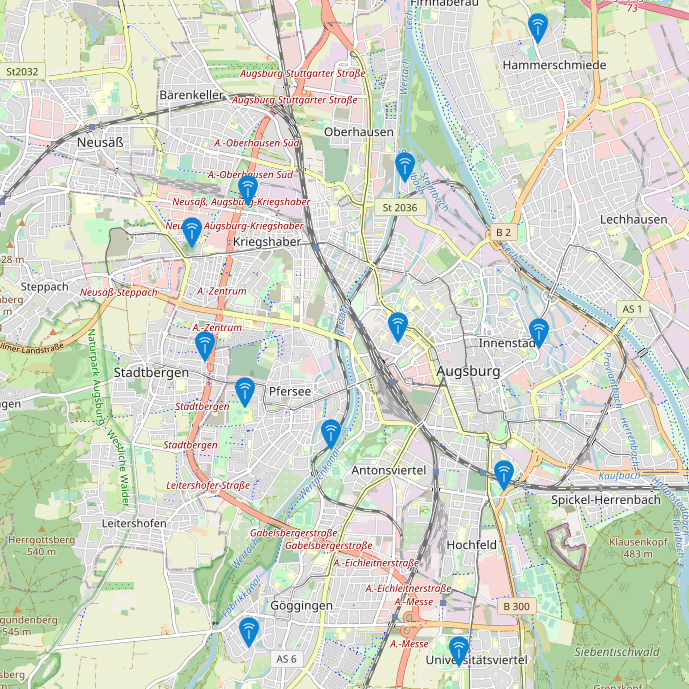
\includegraphics[width=0.65\textwidth]{./images/augsburg-coverage.png}  
    \end{center}
  \vspace{-5pt}
  \caption[The Things Network Gateways: Augsburg]{The Things Network Gateways: Augsburg}
  \caption*{Quelle: {thethingsnetwork.org/map}}
  \label{fig:augsburg-coverage}
  \vspace{-5pt}
\end{figure}

Da viele Städte bereits eine vollständige TTN-Abdeck\-ung vorweisen, können dort große IoT-Szenarien wie Smart Cities oder GPS-Tracking von Fahrrädern realisiert werden, ohne auf die Reichweite eigener Gateways limitiert zu sein. Abbildung \ref{fig:augsburg-coverage} zeigt die vorhandenen Gateways des The Things Network in der Stadt Augsburg im Dezember 2020. Der Ausschnitt der Karte zeigt in etwa 100 $km^2$ Fläche. Es kann davon ausgegangen werden, dass der Großteil der gezeigten Fläche durch die vorhandenen Gateways abgedeckt wird.

Die hohe Anzahl an Gateways und die cloudbasierten Netzwerkkomponenten sorgen außerdem für eine hohe Skalierbarkeit des Netzwerks. Das öffentliche Netzwerk kommt jedoch nicht ohne Nachteile gegenüber eines privaten Netzwerks aus. Der technisch interessanteste ist hierbei die sogenannte \Fachbegriff{Fair Use Policy}. Diese limitiert die erlaubte Nachrichtenanzahl über die lokalen LoRa-Regulierungen hinweg pro Gerät auf 30 Sekunden Uplink und 10 Nachrichten Downlink pro Tag \Zitat{TTN.2020}. Da öffentliche Gateways privat eingesetzt werden gibt es außerdem keine Garantie, dass diese durchgehend verfügbar sind, wodurch ein eigenes Gateway für wichtige Szenarien von essentieller Bedeutung sein kann.

Offensichtlich benötigt ein Netzwerk derartiger Größe ein hohes Maß an Standardisierung der genutzten Software und vor allem der Geräte. Daher wurde von den Entwicklern des The Things Network das Unternehmen The Things Industries gegründet, mit dem Ziel, ein LoRaWAN-Netzwerk mit tatsächlicher globaler Abde\-ckung aufzubauen. Das Unternehmen will dies erreichen, indem es eine ``integrierte Kette aus Produkten und Services'' für die Arbeit mit dem The Things Network bereitstellt. Das einfachste Beispiel hierfür sind die hauseigenen LoRaWAN-Gateways. Diese Gateways werden vorkonfiguriert geliefert und müssen für die Integration in das The Things Network lediglich mit Strom versorgt und in ein IP-basiertes Netzwerk aufgenommen werden. So fällt es Nutzern leicht mit dem Netzwerk zu inter\-agieren, ohne sich mit aufwendigen Konfigurationsarbeiten beschäftigen zu müssen.

Allgemein ist die Nutzung des The Things Network mit der Hardware von The Things Industries die wohl einfachste Möglichkeit des Einstiegs in die Thematik rund um LoRaWAN. The Things Industries bietet jedoch nicht nur Hardware als Produkte an. Da das The Things Network durch die Fair Use Policy gerade für große, kommerzielle Netzwerke oft nicht ausreichend ist, bietet das Unternehmen neben Consulting auch eigene, vollständig gehostete Deployments des The Things Stacks an \Zitat{TTI.2020}. Diese Art von Produkt wird auch als ``Software-as-a-Service'' bezeichnet. Innerhalb des eigenen Netzwerks kann der jeweilige Kunde dann frei agieren und muss lediglich die lokalen LoRa-Regulierungen wie den Duty Cycle (siehe Kapitel \ref{sec:ThHi:technisch}) einhalten.
\clearpage
\chapter{Prototyp}
\label{sec:Prot:first}

Dieses Kapitel beschäftigt sich mit der Planung, dem Aufbau und einer Evaluierung zweier Smart-Building-Prototypen mit LoRaWAN. 

\section{Problemstellung}
\label{sec:Prot:problem}

Selbst wenn man sich nur auf LoRaWAN als IoT-Protokoll beschränkt, sind die Möglichkeiten, ein Smart Building IoT-Netzwerk aufzubauen, unzählig. Neben Netzwerkprovidern, wie beispielsweise Loriot oder aufeinander abgestimmten Komponenten von The Things Industries und dem The Things Stack, existiert eine Vielzahl an Open-Source-Lösungen. Zudem besteht eine IoT-Lösung nicht nur aus dem Netzwerk, über das die Daten versandt werden, sondern einer Datenverwaltung und einer Möglichkeit diese Daten zu visualisieren. Auch hier sind die Auswahlmöglichkeiten nahezu endlos. In dieser Arbeit wird daher ein exemplarischer Prototyp mit möglichst vielen, extern bereitgestellten Services, unter anderem einem öffentlichen LoRaWAN-Netzwerk, und ein zweiter Prototyp mit ausschließlich Open-Source-Software und einem eigenen, privaten Netzwerk, erstellt. Es soll zum Schluss eine begründete Aussage getroffen werden können, welche der Möglichkeiten, beziehungsweise welche Kombination der genutzten Tools, für welche Zwecke am besten geeignet ist.

\section{Verwendete Geräte}
\label{sec:Prot:hardware}

Um ein realistisches Smart Building Szenario mit dem Prototypen nachzustellen, wurden als LoRaWAN-Endgeräte pro Prototyp jeweils ein Temperatur- und Luftfeuchtigkeitssensor (LHT65) und ein Türsensor (LDS01) von der chinesischen Firma Dragino genutzt. Die beiden Sensoren werden in Abbildung \ref{fig:sensors} gezeigt. Der Temperatursensor sendet hierbei alle 20 Minuten eine Nachricht mit drei Messwerten über Temperatur und Luftfeuchtigkeit und weitere Metainformationen wie dem Lade\-stand des Akkus und kostet derzeit in etwa 30€ pro Stück. Der Türsensor hingegen sendet alle 24 Stunden und bei jeder Öffnung und Schließung der Tür eine Nachricht mit dem aktuell Türzustand, der gesamten Anzahl an Türöffnungen, der letzten Öffnungsdauer und ebenfalls Metainformationen wie den Akkustand und ist mit etwa 15€ Stückpreis ebenfalls sehr günstig zu haben. Der ursprüngliche Plan, die Sensoren selbst zu bauen, wurde schnell verworfen, da es nur schwer möglich ist, die Akkulaufzeit und vor allem den Preis der gewählten käuflichen Sensoren zu schlagen.

\begin{figure}[H]
  \vspace{10pt}
  \begin{center}
    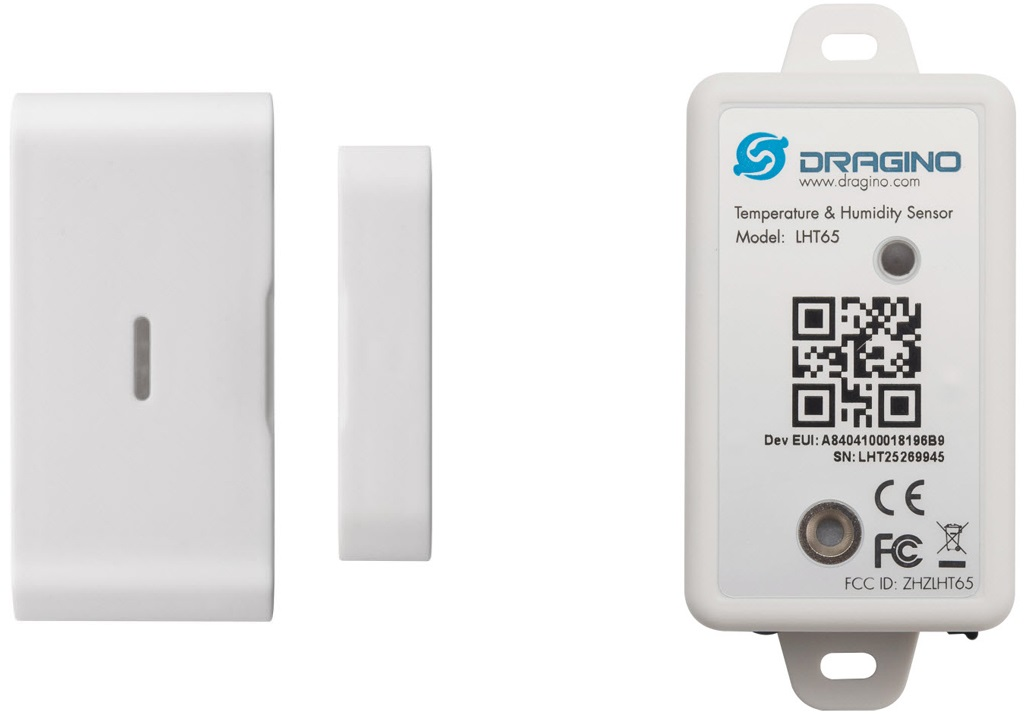
\includegraphics[width=0.6\textwidth]{./images/sensoren.jpg}
  \end{center}
  \vspace{-5pt}
  \caption[Dragino LDS01 und Dragino LHT65 Sensoren]{Dragino LDS01 (links) und Dragino LHT65 (rechts)}
  \caption*{Quelle: {dragino.com/products/products-list.html (bearbeitet)}}
  \label{fig:sensors}
\end{figure}

Auch LoRa-Empfangsstationen gehören zur Hardware hinzu. Für den ersten Prototypen wurde ein offizielles Gateway von The Things Industries verwendet, da derartige Gateways wie in Kapitel \ref{sec:ThHi:ttntti}  beschrieben bereits für das The Things Network vorkonfiguriert sind, und somit die Inbetriebnahme deutlich vereinfachen. Das hier verwendete Gateway ist mit einem Preis von etwa 300€ zwar sehr teuer, es existieren jedoch mittlerweile deutlich günstigere Gateways für das The Things Network. Für den zweiten Prototypen wurde das LPS8 Indoor Gateway von der Firma Dragino genutzt. Dieses Gateway ist für etwa 100€ erhältlich. Abbildung \ref{fig:gateways} zeigt die beiden verwendeten Gateways.

\begin{figure}[H]
  \vspace{10pt}
  \begin{center}
    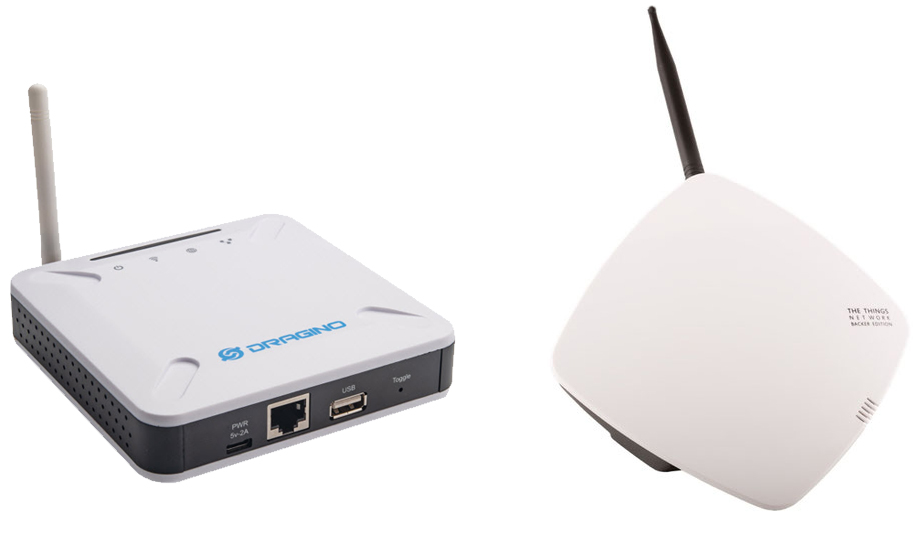
\includegraphics[width=0.85\textwidth]{./images/gateways.jpg}
  \end{center}
  \vspace{-5pt}
  \caption[Dragino LPS8 Gateway und The Things Gateway]{Dragino LPS8 (links) und The Things Gateway}
  \caption*{Quelle 1: {dragino.com/products/lora-lorawan-gateway/item/148-lps8.html (bearbeitet)}}
  \vspace{-10pt}
  \caption*{Quelle 2: {daizy.io/product/the-things-gateway (bearbeitet)}}
  \label{fig:gateways}
\end{figure}

% https://www.dragino.com/media/k2/galleries/148/LPS8-10.jpg
% https://daizy.io/product/the-things-gateway/

\section{Time-Series-Datenbanken}
\label{sec:Prot:timeseriesdb}

Eine wichtige Architekturentscheidung in jedem Softwareprojekt ist die Auswahl einer Datenbank zur Datenverwaltung, so auch in IoT-Projekten. Während im Bereich der Softwareentwicklung der Trend immer mehr in die Richtung der NoSQL-Datenbanken geht, rückt im Bereich des Internet of Things ein neuer Kandidat ins Rampenlicht: Time-Series-Datenbanken. Um dies zu verstehen, gilt es zuerst zu betrachten, wie die Datenverwaltung von IoT-Daten funktioniert. Da meist Daten von vielen verschiedenen Sensoren erhoben werden, diese jedoch nur sporadisch eingesehen werden, ist die Anzahl der Schreiboperationen um ein Vielfaches höher als die der Leseoperationen. Zudem ist für Messwerte immer der Zeitpunkt der Messung interessant, um später zeitabhängige Trends in den Daten erkennen zu können. Unter diesem Aspekt ensteht auch der Name der Datenbanken: es handelt sich um Time-Series-Data, also eine nach der Zeit sortierte Datensequenz wie zum Beispiel den Verlauf der Raumtemperatur eines Gebäudes. 

Allein anhand der Datenstruktur kann die Beliebtheit von Time-Series-Datenbanken im IoT-Bereich leicht erklärt werden. In typischen, relationalen Datenbanken werden Daten in verschiedenen Tabellen mit verschiedenen Verknüpfungen, sogenannten Relationen, gespeichert. Außerdem sind diese Datenbanken primär für Lesezugriffe optimiert. Ein Problem hierbei ist die Struktur der Daten selbst: in relationalen Datenbanken kann pro Tabelle nur ein Schema, also eine Datenstruktur, hinterlegt werden. Somit müssten in großen Projekten unzählige Tabellen erstellt werden.
Da IoT-Daten außerdem meist keinerlei Relationen benötigen und wie bereits erwähnt meist deutlich mehr Schreiboperationen als Lesezugriffe verursachen, sind rela\-tionale Datenbanken nicht perfekt für diesen Usecase geeignet.\\ Genau hier kommen Time-Series-Datenbanken ins Spiel, indem sie genau diese Probleme lösen. Die Datenbanken sind dafür optimiert, viele Schreiboperationen in kurzer Zeit zu tolerieren. Meist werden die Daten in einer Key-Value Struktur hinterlegt, wobei der Key einen Timestamp darstellt. Somit sind gespeicherte Daten nicht nur automatisch zeitlich sortiert, sondern weisen außerdem eine flexible Datenstruktur auf. Der Value kann verschiedenste Werte enthalten und somit Daten von verschiedensten Geräten speichern, ohne mehrere Datenbankinstanzen oder Tabellen zu benötigen. Dies resultiert zwar in einem Mehraufwand bei Datenänderungen, jedoch ist es eher untypisch IoT-Daten wie Messwerte manuell zu verändern.\\ 
Ein weiteres Feature vieler Time-Series-Datenbanken beschäftigt sich mit den Daten selbst. Daten können nach einer bestimmten Lebenszeit automatisch gelöscht werden (Data Lifecycle Management / Retention Policy) oder in bestimmten Zeitblöcken zusammengefasst (Data Summarization) werden. Dies ist interessant, da in IoT-Daten wie zum Beispiel dem Temperaturverlauf eines Gebäudes zwar eine hohe Präzision der letzten Stunden oder Tage, nicht aber der letzten Monate oder Jahre erwünscht ist. Je nach Einstellung könnte also die Datenbank zum Beispiel Daten die älter sind als einen Monat von einem Datenpunkt pro Sekunde zu einem Datenpunkt pro Tag zusammenfassen, wodurch pro Tag nur noch etwa 0.0012\% des vorherigen Speichers verbraucht werden. Diese Präzision reicht jedoch meist völlig aus, um beispielsweise Langzeittrends in den Daten zu erkennen. Eine derartige Logik müsste bei der Nutzung einer normalen relationalen Datenbank aufwendig auf Softwareseite gelöst werden und ist daher meist nicht praktikabel. Nicht zuletzt durch diese Techniken, aber auch durch weitere Optimierungen ist es mit Time-Series-Datenbanken möglich, Abfragen über Millionen von Datenpunkten in wenigen Millisekunden auszuführen. Aus diesen Gründen gehören diese Datenbanken zu den beliebtesten im IoT-Bereich und werden auch hier in beiden Prototypen gewählt. Mehr Informationen über Time-Series-Datenbanken und deren Anwendungsmöglichkeiten können in den Artikeln \cite{TimeSeriesWater.2019} und \cite{TimeSeriesInflux.2020} nachgelesen werden.

\clearpage

\section{Prototyp 1: The Things Network mit Azure IoT Central}
\label{sec:Prot:version1}

Der erste Prototyp wurde unter der Nutzung von möglichst vielen, extern angebotenen Services und Hardwarekomponenten, erstellt. In diesem Kapitel werden eine Beispielarchitektur sowie Erfahrungen und Ergebnisse des Prototyps vorgestellt. Die beiden großen Softwarekomponenten sind hierbei LoRaWAN-seitig das \Fachbegriff{The Things Network} und \Fachbegriff{Microsoft Azure IoT Central} für alle weiteren Funktionen.

\subsection{Erwartungen}
\label{sec:Prot:erwartungen1}

Da in dem Aufbau des Prototypen primär vorkonfigurierte, teilweise sogar kostenpflichtige Services genutzt werden, können klare Erwartungen sowohl an den Aufbau als auch an die Ergebnisse selbst gestellt werden. Die wohl größte Erwartung liegt in der Natur der Cloudservices: es ist nicht nötig, Server selbst aufzusetzen und zu konfigurieren. Auch der LoRaWAN-Stack besteht aus vorkonfigurierten und interoperablen Softwarekomponenten, wie bereits näher in Kapitel \ref{sec:ThHi:ttntti} erklärt wurde. Da außerdem Gateways von \Fachbegriff{The Things Industries} genutzt werden, sollte das Setup der gesamten IoT-Lösung allgemein sehr einfach und kaum zeitaufwendig sein. Eine weitere Erwartung ist eine gute Skalierbarkeit des Systems und vor allem das einfache Hinzufügen neuer Geräte ohne aufwendige Konfiguration. Eine zu diesem Zeitpunkt noch unbehandelte Frage ist die Datenverbindung zwischen dem The Things Network und Azure IoT Central, die im Kapitel \ref{sec:Prot:systemkomponenten1} geklärt wird. Sind die Daten erst einmal in Azure IoT Central, wird eine Vielzahl an nützlichen Features erwartet, um die IoT-Daten zu speichern, zu verwalten oder live zu überwachen. Außerdem soll eine Nutzer- und Rechteverwaltung des Netzwerks möglich sein.

\subsection{Systemkomponenten}
\label{sec:Prot:systemkomponenten1}

Wie bereits erwähnt wird als LoRaWAN-Stack das The Things Network genutzt. Für diesen kleinen Prototypen reicht die Community Edition, also das kostenlose Nutzen des öffentlichen Netzwerks völlig aus. Für sehr große Deployments bietet es sich jedoch an über The Things Industries eine Individuallösung zu beantragen. Zur Verwaltung der Daten wird Azure IoT Central verwendet. Es handelt sich hierbei um die 2018 erschienene IoT-Plattform von Microsoft. Die Entwickler geben an, dass es mit der Plattform möglich sein soll, beliebig große, skalier\-bare und sichere IoT-Anwendungen zu erschaffen, ohne selbst ein Verständnis beziehungsweise Kenntnisse der Cloud zu benötigen. Besonders nützlich ist jedoch die Integration in andere Microsoft Services. So kann beispielsweise auf Sensordaten reagiert werden, indem mit Tools wie Microsoft Flow oder Azure Functions automatisierte Vorgänge ausgeführt werden. Auch Datenvisualisierung mit dem erprobten Tool \Fachbegriff{PowerBI} ist durch diese Integration möglich. Allgemein versucht Azure IoT Central die Komplexität aus IoT-Lösungen zu nehmen und somit das Einrichten einer solchen Lösung zu erleichtern \Zitat{IoTCentral.2019}.

\subsection{Umsetzung}
\label{sec:Prot:umsetzung1}

Die Aufsetzung des ersten Prototypen begann mit der Aktivierung der Endgeräte. Nachdem ein Account im The Things Network angelegt ist, können, wie in Kapitel \ref{sec:ThHi:ttntti} beschrieben, Applications in der sogenannten ``The Things Network Console'', einer Art Kommandozentrale für das eigene Netzwerk, erstellt werden, mit denen später hinzugefügte Geräte assoziiert werden können. Die Aktivierung selbst funktioniert sehr einfach über OTAA oder ABP, wobei in diesem Fall OTAA gewählt wurde. Hierfür muss zuerst die AppEUI in der aktuellen Application hinterlegt werden. Nun kann das Gerät mithilfe eines in der Application eindeutigen Namens, der DevEUI und dem AppKey dem Netzwerk hinzugefügt werden. Sendet das Endgerät nun eine Nachricht, die von einem beliebigen Gateway des The Things Network empfangen wird, erreicht die Nachricht die eigene Application. Betrachtet man die Nachricht, fällt jedoch auf, dass das gesendete Payload hexadezimal dargestellt wird. Dies liegt daran, dass LoRaWAN-Nachrichten meist binär enkodiert werden, um die Nachrichtengröße zu reduzieren und somit mehr Nachrichten pro Tag senden zu können. Um den wahren Inhalt des Payloads zu lesen, kann im The Things Network pro Application eine sogenannte \Fachbegriff{Decoder-Funktion} erstellt werden. Nutzt man selbstgebaute Endgeräte, muss das Enkodieren und Dekodieren selbst programmiert werden, während bei käuflichen Endgeräten die Decoder-Funktion meist mitgeliefert wird. Die gesamte Verwaltung kann durch Rollen und Rechte an verschiedene Nutzer verteilt werden und ist somit selbst für die Zusammenarbeit vieler Personen geeignet.

Nun wird eine Azure IoT Central Anwendung erstellt. Wie bereits angesprochen, muss ein Weg geschaffen werden, Daten aus dem The Things Network in die Azure IoT Central Anwendung weiterzuleiten. Die Lösung hierfür scheint etwas komplizierter als erwartet, jedoch existiert zum aktuellen Zeitpunkt keine einfachere Möglichkeit. Microsoft Azure veröffentlichte für derartige Vorhaben die ``iotc-device-bridge'' als Open-Source-Projekt auf GitHub\footnote{\url{github.com/Azure/iotc-device-bridge}}, welche es Nutzern ermöglicht, Daten aus anderen IoT-Cloud-Services an Azure IoT Central zu senden. Das Funktionsprinzip selbst ist hierbei recht einfach. Die Device Bridge wird als Azure Function, also als eine Azure Ressource bereitgestellt. Bei Azure Functions handelt es sich um eine Möglichkeit, Programmcode beim Aufkommen verschiedenster Events auszuführen, ohne dafür einen Server aufsetzen zu müssen. So ist es beispielsweise möglich, HTTP-basierte Endpunkte mit Azure Functions zu verwirklichen \Zitat{AzureFunction.2016}. Genau dieser Funktionalität macht sich die Device Bridge zunutze. Die Applikation empfängt Nachrichten via HTTP vom The Things Network und leitet diese durch die Azure Infrastruktur an die IoT Central Application weiter. Viele IoT-Cloud-Services, wie auch der Application Server des The Things Network bieten sogenannte Integrations an. Integrations sind Möglichkeiten, Daten aus dem The Things Network an andere Dienste weiterzuleiten. Naheliegend war in der Erstellung dieses Prototypen die Nutzung der HTTP Integration, die eingehende Nachrichten an einen HTTP-Endpoint weiterleiten kann. Somit musste lediglich die Azure Device Bridge als HTTP-Endpoint für diese Integration konfiguriert werden. Nun finden die Daten ihren Weg von den LoRaWAN-Endgeräten bis hin zur IoT Central Anwendung.

Um eingehende Daten in Azure IoT Central nutzen zu können, müssen vorerst sogenannte ``Device Templates'' erstellt werden. Diese stellen ein semantisches Mapping der Rohdaten auf eine virtuelle Kopie des genutzten Gerätes dar. Hier werden alle vorhandenen Werte und deren Einheiten strukturiert festgelegt. Dies bietet den großen Vorteil, dass Nutzer bei der Einsicht der Daten kein genaues Verständnis über die Daten benötigen und keine Rohdaten interpretieren müssen. Sendet ein Gerät zum ersten Mal eine Nachricht, muss das Gerät manuell in IoT Central einem Device Template zugeordnet werden. Von diesem Zeitpunkt an können die Daten sinnvoll genutzt werden. Das Hinzufügen neuer Geräte funktioniert also ohne aufwendige Konfiguration und erfordert lediglich das Registrieren des Geräts im The Things Network und die Zuweisung zu einem Device Template in Azure IoT Central.

\begin{figure}[H]
  \vspace{10pt}
  \begin{center}
    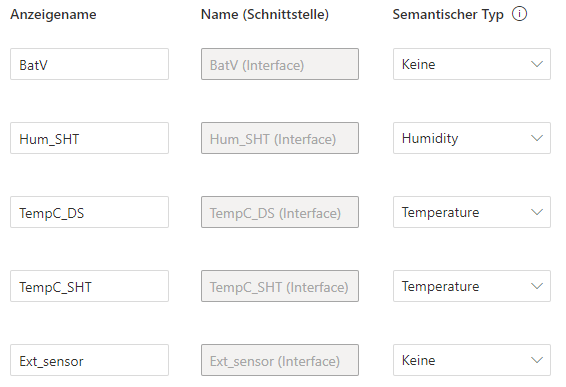
\includegraphics[width=0.8\textwidth]{./images/device-template.png}  
    \end{center}
  \vspace{-5pt}
  \caption[IoT Central Device Template]{IoT Central Device Template}
  \label{fig:device-template}
  \vspace{-10pt}
\end{figure}

Abbildung \ref{fig:device-template} zeigt das Device Template des im Prototypen genutzten Temperatursensors. Es fällt auf, dass beispielsweise dem Attribut ``TempC\_DS'', also einem Temperaturwert, der semantische Typ ``Temperature'' zugeordnet ist. Somit muss der Wert von Endnutzern nicht mehr als numerischer Wert interpretiert werden.

Die wohl einfachste Nutzung der Daten ist die Visualisierung. Hierfür können ganze Dashboards zusammengestellt werden, in denen die Daten durch verschiedene Graphen oder Ansichten dargestellt werden. Das Erstellen solcher Visualisierungen ist hier sehr einfach, da IoT Central durch die Device Templates bereits versteht, welche Visualisierungen für die jeweilige Datenstruktur möglich ist. So ist beispielsweise ein Graph für Temperaturdaten sehr geeignet, während für ein Protokoll aus Zuständen wie Türöffnungen eher eine textuelle Liste sinnvoll ist. 

\begin{figure}[H]
  \vspace{10pt}
  \begin{center}
    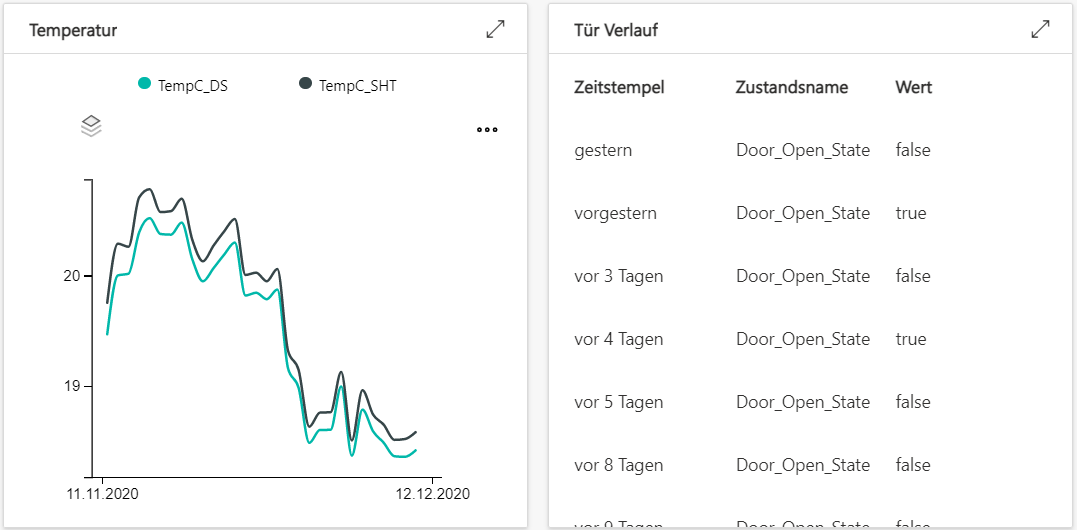
\includegraphics[width=1.0\textwidth]{./images/iotcentral-dashboard.png}  
    \end{center}
  \vspace{-5pt}
  \caption[IoT Central Dashboard]{IoT Central Dashboard}
  \label{fig:iotcentral-dashboard}
  \vspace{-10pt}
\end{figure}

Es gilt hier jedoch zu erwähnen, dass die Möglichkeiten zur Datenvisualisierung zum heutigen Stand noch sehr limitiert und häufig nur wenig konfigurierbar sind. In Abbildung \ref{fig:iotcentral-dashboard} ist beispielsweise zu erkennen, dass die Temperaturdaten anschaulich visualisiert sind, während der Zustand des Türsensors lediglich in einer Tabelle dargestellt wird. Für einfache Szenarien, vor allem dann, wenn die Visualisierung keine große Anforderung ist, reichen die existierenden Möglichkeiten jedoch völlig aus. Neben den Anzeigen eines Dashboards können außerdem Daten auch sehr detailliert über den Analyse-Tab eingesehen werden. Auch Langzeitentwicklungen oder Extremwerte sind hier leicht festzustellen.


Die wohl positivste Überraschung der IoT Central Anwendung war die sehr nützliche Anbindung an die gesamte Microsoft-Infrastruktur. Dies fiel erstmals bei der Einrichtung von Alerts bei Überschreitungen von festgelegten Temperatur- und Luftfeuchtigkeitslimits von festgelegten Limits auf. In IoT Central können nicht nur diese Regeln, sondern auch unzählige Aktionen wie zum Beispiel der Versand einer dynamisch gefüllten E-Mail oder das Aufrufen eines Webhooks konfiguriert werden. Auch das Exportieren von Daten in Azure Blob Storages zur permanenten Datenspeicherung oder Azure Event Hubs für Event Processing und vieles mehr ist mit IoT Central unkompliziert möglich. IoT Central speichert Daten selbst nur 30 Tage lang in einer Time-Series-Datenbank, weswegen ein solcher Export für Szenarien mit Bedarf an Langzeitspeicherung der Daten essentiell wichtig ist. Durch das Exportieren der Daten in die Azure Infrastruktur können nun eine Vielzahl an zusätzlichen Services, wie beispielsweise PowerBI zur besseren Datenvisualisierung, genutzt werden. Auch die Nutzerverwaltung ist direkt an Microsoft gekoppelt. Somit können Zugriffsrechte an Microsoft-Accounts verteilt werden, was gerade in Situationen, in denen bereits eine oft firmeninterne Microsoft-Infrastruktur besteht, sehr hilfreich ist.

\subsection{Architekturübersicht}
\label{sec:Prot:architektur1}

Nachdem nun alle Hardware- und Softwarekomponenten im System sind, hilft es sich einen Überblick über die bisherige Architektur zu schaffen.

\begin{figure}[H]
  \vspace{10pt}
  \begin{center}
    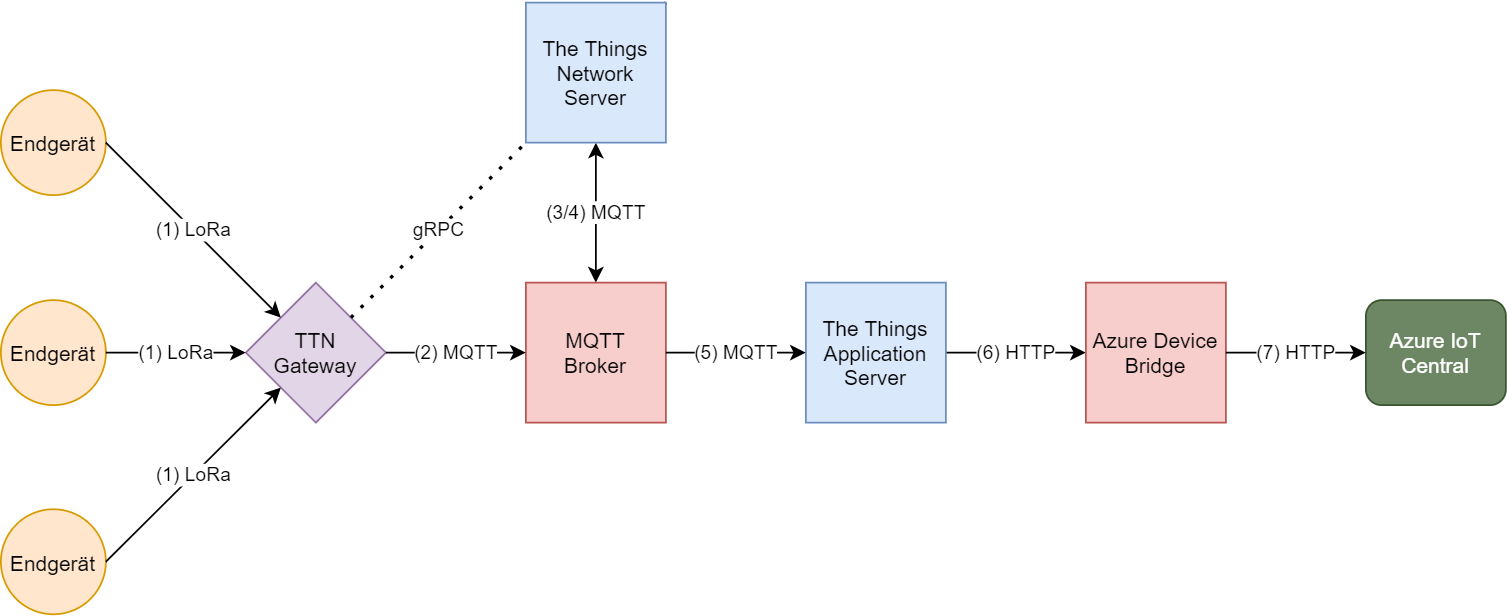
\includegraphics[width=1\textwidth]{./images/ttn-architecture.png}
  \end{center}
  \vspace{-5pt}
  \caption[Prototyp 1: Architekturübersicht]{Prototyp 1: Architekturübersicht}
  \label{fig:ttn_prototype_architecture}
  \vspace{-10pt}
\end{figure}

In Abbildung \ref{fig:ttn_prototype_architecture} ist der Datenfluss einer Uplink-Nachricht eines Endgeräts mit den jeweils genutzten Protokollen durchnummeriert. Es gilt hier zu erwähnen, dass in der Abbildung aus Gründen der Übersichtlichkeit nur Netzwerkkomponenten, die direkt am Datenversand beteiligt sind, dargestellt sind. Dieser beginnt mit dem Datenversand des Endgeräts zum The Things Gateway über LoRa. Empfangen mehrere Gateways im Netzwerk die Nachricht, werden Duplikate später im Network Server gefiltert und können hier somit ignoriert werden. Das Gateway kann durch die Nutzung des Gateway Connector Protocols wahlweise über gRPC Nachrichten direkt an den Network Server oder via MQTT über den Message Broker senden. Erreicht den Network Server eine Nachricht, arbeitet dieser seine Aufgaben ab, wie beispielsweise das Filtern von Duplikaten oder das Validieren der Nachricht. Anschließend leitet der Network Server erneut über den MQTT Broker die nun verarbeitete Nachricht an den Application Server weiter. Dieser ist die letzte Komponente im LoRaWAN-Stack und leitet die Daten über die HTTP Integration an die Azure Device Bridge weiter. Diese Device Bridge, die intern eine Azure Function darstellt, speist diese Daten nun über das HTTP-Protokoll in Azure IoT Central ein. 

\subsection{Evaluation}
\label{sec:Prot:procontra1}

Der erste Prototyp fällt durch einige Stärken sehr positiv auf. Gerade in kleinen Projekten ist die Nutzung des The Things Network ein großer Vorteil, sofern man sich in Reichweite eines öffentlichen Gateways befindet. Da die Kosten für ein eigenes Gateway dadurch wegfallen und lediglich die Endgeräte finanziert werden müssen, handelt es sich hier um eine der günstigsten Möglichkeiten ein LPWA-Netzwerk aufzubauen. Hier gilt es zu erwähnen, dass es keinerlei Garantie gibt, dass ein fremdes Gateway konstant aktiv bleibt, und somit spontane Ausfälle des Netzwerks möglich sind. Ist eine solche Garantie erwünscht, muss also trotz des öffentlichen Netzwerks ein eigenes Gateway eingerichtet werden. Ist ein großes Netzwerk angestrebt, steht neben der Community des The Things Network das Unternehmen The Things Industries für Consulting und fertige Lösungen zur Verfügung, was ebenfalls einen großen Vorteil darstellt. Auch die genutzten Softwarekomponenten bieten einige hilfreiche Features. Sowohl das The Things Network als auch Azure IoT Central Anwendungen sind ausreichend skalierbar und somit für jede Netzwerkgröße geeignet. Speziell Azure IoT Central als IoT Plattform überzeugt durch eine Vielzahl nützlicher Eigenschaften. Besonders hilfreich ist das semantische Mapping von Daten auf Gerätevorlage, wodurch Nutzer keinerlei Wissen über die Datenstruktur benötigen. Außerdem ist IoT Central sehr tief in die Microsoft Infrastruktur eingebettet und erlaubt eine Anbindung der IoT Plattform an unzählige Features wie E-Mail-Alerting, Stream Analytics (Analyse von Echtzeitdaten) oder Langzeitspeicherung. 

In der Umsetzung und Nutzung des Prototypen sind jedoch auch viele Nachteile aufgefallen. Der wohl offensichtlichste dieser Nachteile ist, dass durch die Nutzung von Microsoft Azure Services, und bei großen Deployments auch beim The Things Network, Kosten entstehen. In diesem Kapitel soll jedoch der Fokus auf dem Netzwerk selbst bleiben. Das The Things Network limitiert die Sendezeit aller Geräte strenger als die meisten lokalen Regulierungen durch den Duty Cycle dies tun. So werden jedem Gerät lediglich 30 Sekunden Uplinkzeit und 10 Nachrichten Downlink pro Tag zugeteilt. Nimmt man beispielsweise an, dass eine Nachricht im Schnitt 100 Millisekunden Airtime benötigt, können somit nur 300 Nachrichten pro Tag pro Gerät gesendet werden. Zwar ist dies für viele IoT-Lösungen ausreichend, stellt jedoch eine deutliche Einschränkung gegenüber anderen Techniken dar. Im Prototypen beispielsweise sendet der Temperatur- und Luftfeuchtigkeitssensor alle 20 Minuten eine Nachricht also 72 am Tag und ist somit nicht von der Einschränkung betroffen. \\
Eine sehr unangenehme Eigenschaft des The Things Network ist außerdem, dass bis zum aktuellen Zeitpunkt pro Applikation nur eine Decoder-Funktion erstellt werden kann. Erstellt man also beispielsweise eine Appli\-kation für Temperaturdaten, können nur Geräte mit der gleichen Datenstruktur genutzt werden. Existieren verschiedene Sensortypen müssen also mehrere Applikationen für den eigentlich gleichen Zweck erstellt werden, was sehr schnell sehr unübersichtlich werden kann. Außerdem ist der externe Zugriff auf die Daten sehr umständlich. Zwar veröffentlicht der Application Server die Daten über einen MQTT Broker, jedoch müssen sich Consumer hier pro Application mit verschiedenen Zugangsdaten authentifizieren, was oft nicht praktikabel ist. Um dies zu umgehen, können Integrations, wie in diesem Fall die HTTP-Integration genutzt werden, jedoch muss diese ebenfalls pro Applikation erstellt werden, was erneut eine Fehlerquelle darstellt und bei Änderung der Ziel-URL aufwendig manuell geändert werden muss.\\
Auch die Azure Device Bridge ist ein großer Nachteil dieses Prototypen: der Verwalter des Netzwerks benötigt Softwareentwicklungs- und Azure-Kenntnisse um die Device Bridge aufzusetzen und warten zu können. Auch Azure IoT Central kommt nicht ganz ohne Nachteile aus. So sind die Visualisierungsmöglichkeiten innerhalb der Anwendung sehr gering und zwingen den Nutzer für anschaulichere Dashboards externe Tools wie Microsoft PowerBI zu nutzen, was deutlich mehr Setup erfordert. Außerdem zwingt das semantische Mapping auf Gerätevorlagen den Nutzer gewisse Datentypen zu nutzen. So überträgt der im Prototypen verwendete Sensor die Temperatur und Luftfeuchtigkeit als String, um die Messgenauigkeit beizubehalten, Gerätevorlagen in IoT Central können diese Werte jedoch nur als Zahl interpre\-tieren. Um dies zu umgehen, muss die mitgelieferte Decoder-Function verändert werden und den Wert in einen anderen Datentypen umwandeln. Da bisher keine einheitlichen Normen für Datenformate von IoT-Daten existieren und somit jeder Hersteller ein eigenes Format nutzt, kann dies schnell zu Problemen führen. Außerdem ist der gesamte Softwarestack eine Art Blackbox, da keinerlei Zugriff auf Logs möglich ist. Somit ist es schwer Fehlerquellen im System zu finden. Es gilt auch zu erwähnen, dass dieser Prototyp nur mit Internetzugriff funktioniert, also keine IoT-Netze in einem lokalen Intranet möglich sind.

Allgemein gilt es gerade beim The Things Network hervorzuheben, dass es sich hier weniger um ein fertiges Produkt sondern um die Vision, ein globales, öffentliches LPWA-Netzwerk aufzubauen, handelt. Für fehlende oder noch nicht perfekte Features werden ständig neue Updates veröffentlicht, wodurch das The Things Network in der Zukunft eine potenzielle Lösung für LoRaWAN-Netzwerke jeder Art darstellt. Die Evaluation bewertet lediglich den aktuell Stand des The Things Network für IoT-Lösungen.

\newpage

\section{Prototyp 2: ChirpStack mit InfluxDB und Grafana}
\label{sec:Prot:version2}

Der zweite Prototyp wurde im Vergleich zum ersten ausschließlich mit Open-Source-Software aufgesetzt und nutzt neben einer Azure VM für das Hosting der Anwendung keine externen Services. In diesem Kapitel werden vorerst Erwartungen an den Prototypen gestellt. Anschließend wird eine Alternative zum The Things Network und weitere Software zur Datenverwaltung vorgestellt. Darauf folgen wie beim ersten Prototypen die Umsetzung, Architektur und eine Evaluation des Ergebnisses. In diesem Prototypen werden die Open-Source-Anwendungen \Fachbegriff{ChirpStack} als LoRaWAN-Stack, InfluxDB als Datenbank und Grafana zur Datenvisualisierung verwendet. 

\subsection{Erwartungen}
\label{sec:Prot:erwartungen2}

Da der Aufbau dieses Prototypen keinerlei extern angebotene Services nutzt, kann davon ausgegangen werden, dass das Aufsetzen hier aufwendiger und komplexer ist als beim ersten Prototypen. So müssen unter anderem eigene Server aufgesetzt, konfiguriert und gewartet werden. Hier sind auch Zugriffsrechte und allgemeine Sicherheit vor Angriffen ein großes Thema, welches unter keinen Umständen vernachlässigt werden sollte. Auch das Inbetriebnehmen des eigenen LoRaWAN-Stacks stellt einen erhöhten Aufwand dar, da diese Arbeit im ersten Prototypen durch die Nutzung des The Things Network komplett weggefallen ist. Außerdem muss neben den Endgeräten aufgrund des eigenen privaten LoRaWAN-Netzwerks zwangsweise ein eigenes Gateway gekauft werden. Es wird davon ausgegangen, dass sich lediglich an den Duty Cycle, nicht aber an spezielle Regelungen wie die Fair Use Policy des The Things Network, gehalten werden muss und somit eine höhere Nachrichtenanzahl pro Gerät pro Tag möglich ist. Da vollständige Kontrolle über die Datenbank gegeben ist, wird davon ausgegangen, dass das Festlegen einer für den eigenen Usecase geeigneten Datenstruktur möglich ist. Durch die Nutzung von Grafana wird erwartet, eine Vielzahl an Visualisierungsmöglichkeiten nutzen zu können und alle erwünschten Darstellungen aufbauen zu können. Allgemein wird damit gerechnet, durch das eigene Hosting der Services volle Kontrolle und vor allem Überblick durch Logs über das System zu haben und somit beispielsweise Fehler einfach finden und beheben zu können. Außerdem wird davon ausgegangen, dass dieser Prototyp auch offline in einem Intranet funktionieren könnte.

\subsection{Systemkomponenten}
\label{sec:Prot:systemkomponenten2}

Im Aufbau dieses Prototypen werden eine Vielzahl neuer Softwarekomponenten genutzt, die in diesem Kapitel vorgestellt werden. Es handelt sich bei jeder dieser Komponenten um Open-Source-Anwendungen, die völlig kostenlos genutzt werden können.

\subsubsection{ChirpStack} % Highlights und Architektur aus Doku

Die wohl wichtigste der Komponenten für den Prototypen ist der \Fachbegriff{ChirpStack}. Hierbei handelt es sich um einen LoRaWAN-Stack mit allen in Kapitel \ref{sec:ThHi:architektur} genannten Bauteilen, wobei der Join Server mit in den Application Server integriert ist. Die Funktionen des ChirpStack ähneln denen des The Things Network sehr stark und unterscheiden sich meist nur in Quality-of-Life-Änderungen. Neben dem einzelnen Deployment der Gateway Bridge, des Network Servers und des Application Servers ist außerdem ein Operating System (OS) verfügbar. Das linuxbasierte OS erleichtert die Inbetriebnahme eines LoRaWAN-Stacks stark, indem ein Großteil der Konfigurationsarbeit wegfällt. Da dieser Prototyp aber in einer Azure VM bereitgestellt werden sollte, wurden die einzelnen Komponenenten hier bevorzugt.

\begin{figure}[H]
  \vspace{10pt}
  \begin{center}
    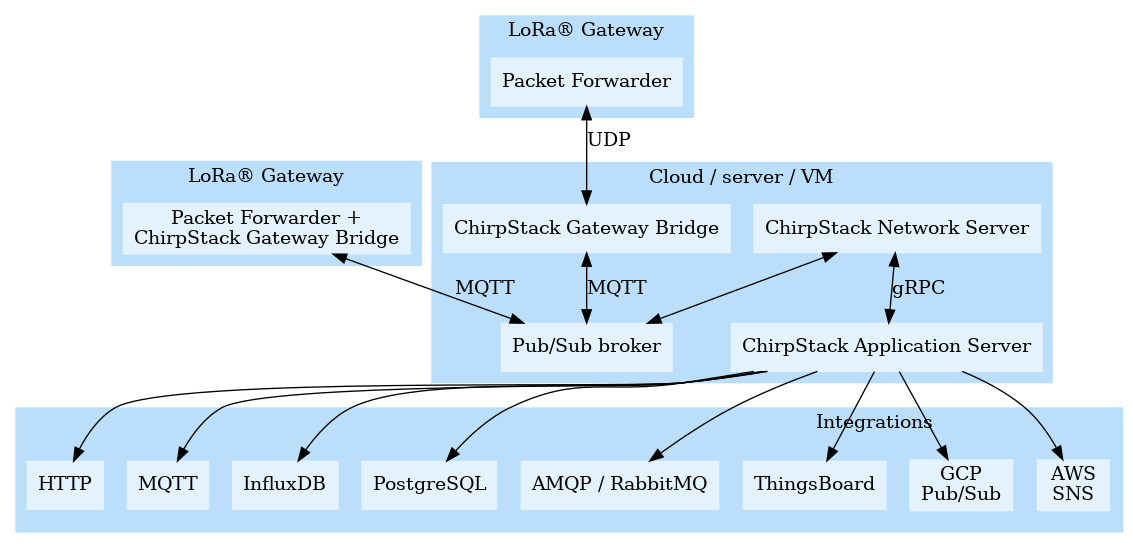
\includegraphics[width=1\textwidth]{./images/chirpstack_architecture.png}
  \end{center}
  \vspace{-5pt}
  \caption[ChirpStack Architektur]{ChirpStack Architektur}
  \caption*{Quelle: {chirpstack.io/static/img/graphs/architecture.dot.png}}
  \label{fig:chirpstack_architecture}
  \vspace{-10pt}
\end{figure}

Wie aus Abbildung \ref{fig:chirpstack_architecture} hervorgeht, ist die Architektur des ChirpStack der des The Things Network sehr ähnlich. Im Zentrum steht ein Pub-Sub-Message-Broker, im Speziellen ein MQTT Broker. Gateways, die nur den Packet Forwarder installiert haben, senden per UDP Nachrichten an die Gateway Bridge, während Gateways, die diese Komponente bereits installiert haben, Nachrichten direkt an den MQTT Broker weiterleiten. Die Gateway Bridge wandelt das LoRa-Datenformat in JSON oder Protobuf um, da dies die vom ChirpStack genutzten Formate zur Weiterverarbeitung sind. Über den Message Broker wandern die Daten weiter in den Network Server. Nachdem dieser seine Aufgaben abgearbeitet hat, sendet der Network Server die Daten weiter an den Application Server. Dies geschieht nicht wie beim The Things Network über den Message Broker, sondern über einen gRPC-Call. Im Application Server können nun wie beim The Things Network Integrations genutzt werden, um die Daten extern erreichbar zu machen \Zitat{ChirpArch.2020}.

\subsubsection{MQTT Consumer} % Erklärung zu TICK bzw TIG#
\label{sec:Prot:systemkomponenten2:mqttcons}
Um Daten vom ChirpStack in eine externe Datenbank zu bewegen, gibt es im Allgemeinen zwei Herangehensweisen. Zum einen können ähnlich zum The Things Network diverse Integrations genutzt werden, die Daten direkt in ein kompatibles Ziel wie beispielsweise HTTP-Endpoints schreiben. Da in diesem Prototypen eine InfluxDB als Datenbank verwendet wird, eignet sich hierfür die InfluxDB-Integration. Diese erfordert kaum Setup und kann Daten in eine beliebige, vom ChirpStack Application Server erreichbare, InfluxDB-Instanz schreiben. Mit dieser Methode macht sich jedoch schnell ein Problem bemerkbar. In der aktuellen ChirpStack-Version ist es nicht möglich, eine eigene Datenstruktur vorzugeben. Durch die relativ unstrukturierte vorgegebene Speicherung wird es später vor allem für Nutzer, die die Daten nicht genau kennen, sehr schwer, diese sinnvoll zu nutzen. Aus diesem Grund wurde ein eigenes Tool\footnote{\url{r-n-d.informatik.hs-augsburg.de:8080/loisbois/mqtt\_lorawan\_consumer}} in der Programmiersprache Go geschrieben, welches die Tatsache nutzt, dass der Application Server Daten stets über die MQTT-Integration an den Message Broker weiterleitet und diese somit über MQTT zugänglich macht. Dieses Tool ist ein MQTT Client mit der Aufgabe, Daten aus dem ChirpStack zu empfangen, diese strukturiert umzuformen und anschließend in das InfluxDB-Line-Protocol, welches im nächsten Kapitel \ref{sec:Prot:systemkomponenten2:influx} weiter erklärt wird, zu übersetzen. 

Über eine Konfigurationsdatei können neben Datenquelle und -ziel die Werte, die verwendet werden sollen, hinterlegt werden. Dies ist besonders wichtig, da es im LoRaWAN-Bereich hierfür erneut keine einheitliche Benennung gibt. So werden Messdaten (also das entschlüsselte LoRaWAN-Payload) im The Things Network unter dem Key ``payload\_fields'' gespeichert, während der ChirpStack den Key ``object'' für diesen Zweck verwendet. Ist in der Konfigurationsdatei eine InfluxDB-Instanz konfiguriert, schreibt das Tool die umgewandelten Daten über die HTTP-Schnittstelle der InfluxDB in den Speicher. Gibt man in der Konfiguration als MQTT-Topic ``application/+/device/+/event/up'' an, wobei das Plus-Zeichen jeweils eine sogenannte Wildcard, also einen beliebigen Wert, darstellt, empfängt der MQTT Consumer die Daten aller registrierten Endgeräte.

Dadurch dass die Programmiersprache Go genutzt wurde kann das Tool zu einer ausführbaren Binary-Datei kompiliert werden. Um diese noch vollständig system\-unabhängig zu machen, also nicht pro Endgerät neu kompilieren zu müssen, wurde außerdem ein eigenes Docker Image erstellt. Da das Docker Image lediglich eine Binary-Datei ausführen muss, und somit keinerlei Systemdateien benötigt, ist das Image mit einer Größe von unter 10 Megabyte außerdem sehr schlank.


\subsubsection{InfluxDB}
\label{sec:Prot:systemkomponenten2:influx}

In Kapitel \ref{sec:Prot:timeseriesdb} wurde bereits erwähnt, dass Time-Series-Datenbanken im IoT-Umfeld immer beliebter werden. In diesem Kapitel wird InfluxDB, eine der verbreitetsten dieser Datenbanken, behandelt.

InfluxDB ist eine, in der Programmiersprache Go entwickelte, Open-Source Time-Series-Datenbank der Firma InfluxData. Die Datenbank wurde im Vergleich zu einer Vielzahl ähnlicher Datenbanken seit Beginn der Enwicklung als Time-Series-DB geplant und dafür optimiert. Die DB unterstützt alle typischen Time-Series-Funktionen wie das Löschen alter Daten oder die Zusammenfassung von Daten in bestimmten Zeiträumen und überzeugt durch Einfachheit, aber auch durch ihre Leichtgewichtigkeit. So können selbst ressourcenarme Geräte wie ein Raspberry Pi hunderte von Sensoren, welche gleichzeitig in eine Datenbank auf dem Einplatinencomputer schreiben, unterstützen \Zitat{TimeSeriesWater.2019}. 

\begin{figure}[H]
  \vspace{10pt}
  \begin{center}
    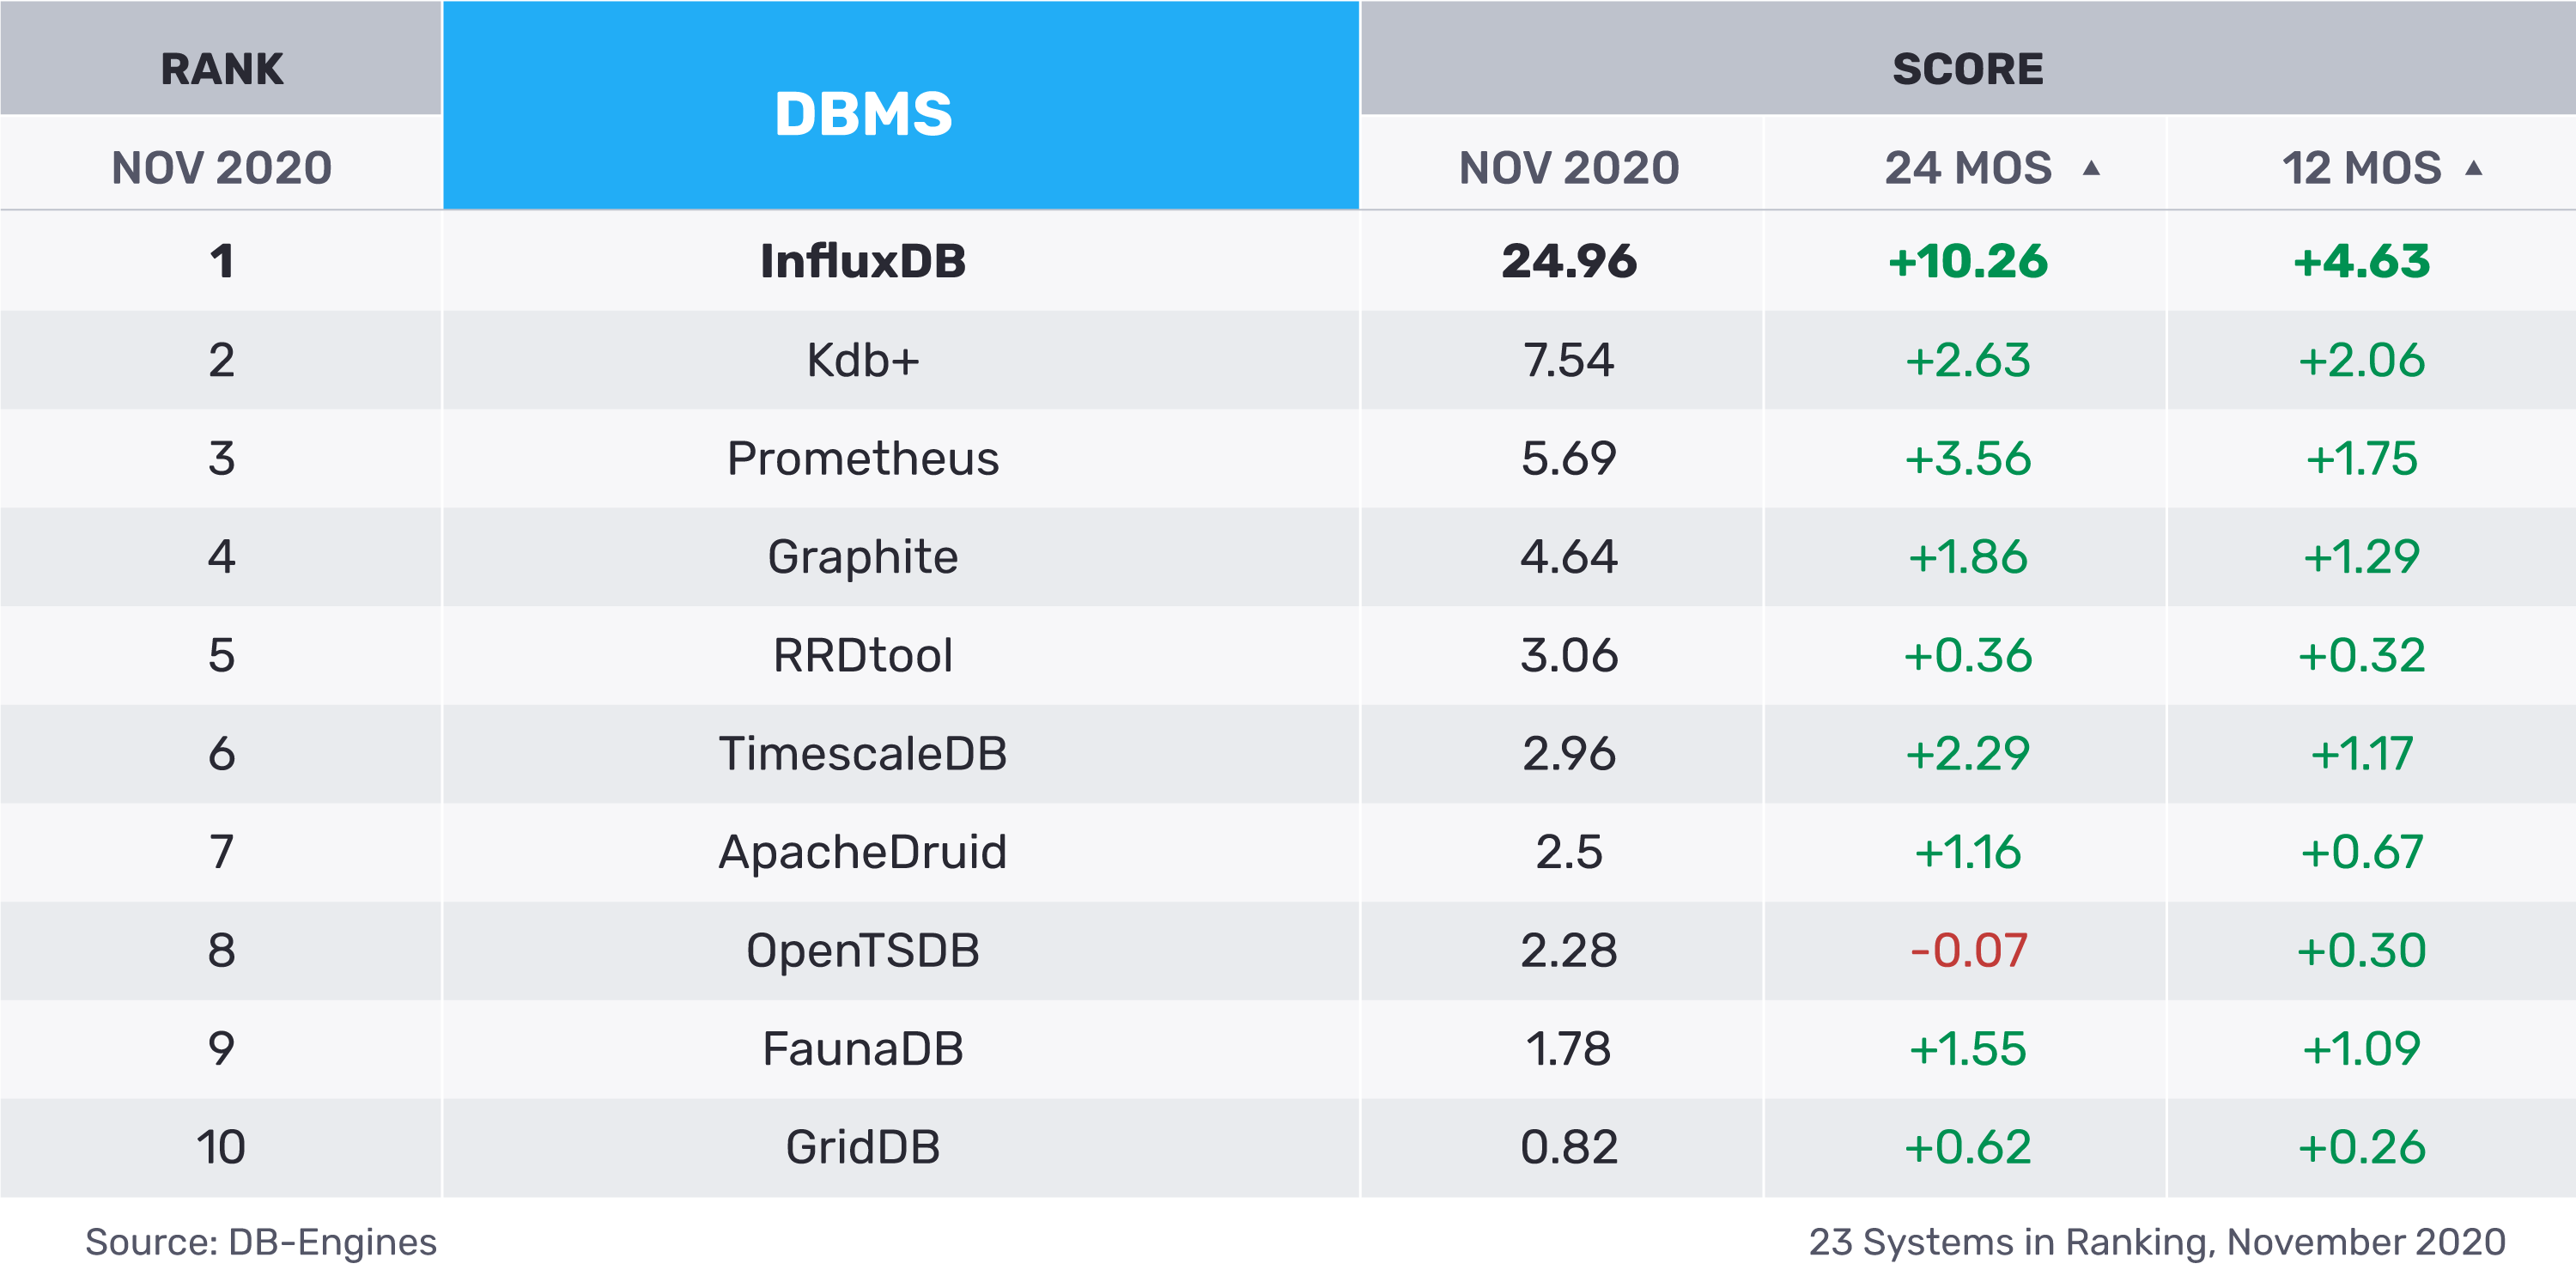
\includegraphics[width=1.0\textwidth]{./images/timeseries_ranking.png}
  \end{center}
  \vspace{-5pt}
  \caption[DB-Engines: Ranking von Time-Series-Datenbanken]{DB-Engines: Ranking von Time-Series-Datenbanken}
  \caption*{Quelle: {influxdata.com/time-series-database}}
  \label{fig:timeseries_ranking}
  \vspace{-10pt}
\end{figure}

InfluxDB wird als beliebteste Time-Series-DB bezeichnet und wird, wie Abbildung \ref{fig:timeseries_ranking} zu entnehmen ist, von unabhängigen Websiten oft mit Abstand auf den ersten Platz im Ranking gesetzt. In den beiden Spalten auf der rechten Seite der Grafik kann die Entwicklung des jeweiligen Scores der letzten 12 und 24 Monate abgelesen werden.

In einer InfluxDB existieren im Allgemeinen drei verschiedene Ressourcen: Nutzer, Retention Policies und Points. Wie in anderen vergleichbaren Datenbanken sind Zugriffs- und Verwaltungsrechte an Nutzer gebunden. Retention Policies bestimmen unter anderem, wie lange die Datenbank Daten speichert, welche Daten zusammengefasst werden können und in welchen Zeitabständen zusammengefasst werden soll. Auch wie Daten zusammengefasst werden kann hier konfiguriert werden, wobei meist der Durchschnitts- oder Maximalwert des Zeitfensters gewählt wird. Abschließend kommt das Kernstück einer jeden Datenbank: die Daten selbst. In einer InfluxDB werden Datenpunkte als \Fachbegriff{Points} bezeichnet.\\
Jeder Point besteht aus einem \Fachbegriff{Measurement}, einem \Fachbegriff{Tagset}, einem \Fachbegriff{Fieldset} und einem \Fachbegriff{Timestamp}. Das Measurement ist dafür da, zusammengehörige Datenpunkte gruppieren zu können. Im Falle des Prototypen wurde die Datenstruktur so gewählt, dass das Measurement den Applikationstyp, zum Beispiel "temp-hum", darstellt. So können alle Temperatur- und Luftfeuchtigkeitsdaten des Systems über das gleiche Measurement gefunden werden. Mit dem Tagset können in einem Key-Value-Format Metainformationen zu dem Point gespeichert werden. Im Prototypen war ein solches Tag der ``deviceName'', der innerhalb eines LoRaWAN-Netzwerks eindeutig ist.\\
Nun kann ein einzelnes Gerät schnell gefunden werden, da zuerst die Auswahl durch das Measurement auf den Applikationstypen reduziert werden kann, und das einzelne Gerät nur noch aus einer stark reduzierten Datenmenge gefiltert werden muss. Die InfluxDB baut außerdem über das Tagset eine Indexstruktur auf, um Lesezugriffe deutlich zu beschleunigen. Im Fieldset finden sich nun die eigentlichen Daten des Points. Auch hier werden Daten in einem Key-Value-Format hinterlegt, jedoch nicht indiziert, da hier primär Schreiboperationen vorgenommen werden. Der letzte Teil des Points ist ein Timestamp, der mit konfigurierbarer Genauigkeit den Zeitpunkt der Aufnahme des Points speichert. 

Points werden in einer InfluxDB durch das Line Protocol serialisiert. Dieses Serialisierungsformat enthält alle vier Komponenten eines Points und beginnt mit dem Namen des Measurements. Nun folgt optional das Tagset. Existieren Tags, werden diese direkt nach dem Measurement mit der Schreibweise ``,key=value'' notiert und aneinandergereiht. Enthält ein Key oder ein Value Leer- oder Sonderzeichen, muss die Zeichenfolge in Anführungszeichen gesetzt werden. Hier gilt es, das führende Komma zu beachten. Ein Leerzeichen beendet das Tagset und beginnt somit das Fieldset welches im gleichen Format wie das Tagset notiert wird, wobei das erste Element auf das führende Komma verzichtet. Hier gilt es zu beachten, dass das Fieldset im Gegensatz zum Tagset nie leer sein darf. Nach einem weiteren Leerzeichen folgt der Timestamp. Ein Point im Line Protocol aus dem Prototypen wird in Abbildung \ref{fig:lineprotocol} gezeigt.

\begin{figure}[H]
  \vspace{10pt}
  \begin{center}
    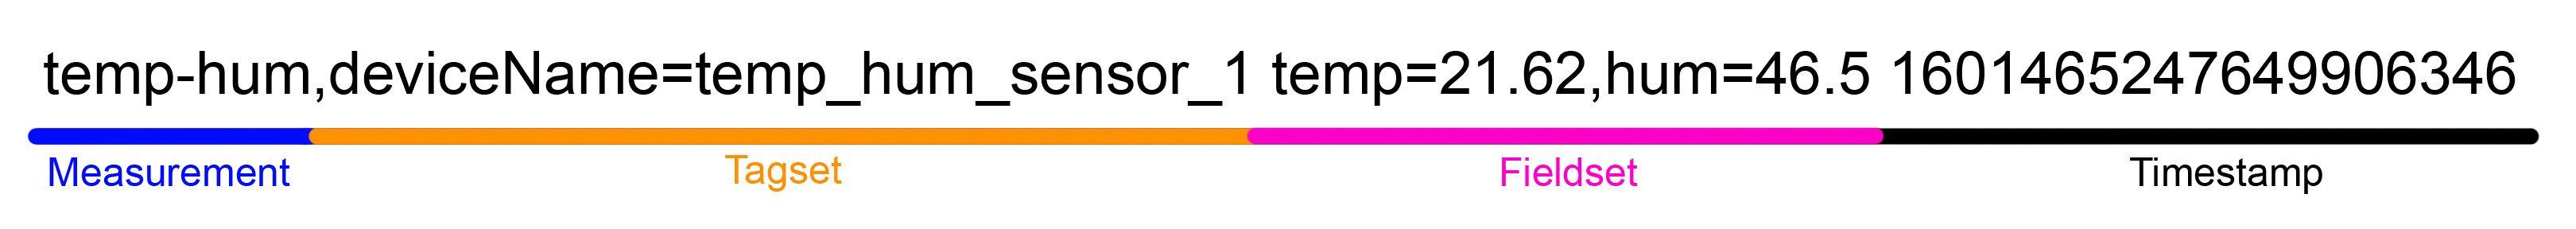
\includegraphics[width=1.0\textwidth]{./images/LineProtocol.jpg}
  \end{center}
  \vspace{-5pt}
  \caption[Datenpunkt im Influx Line Protocol]{Datenpunkt im Influx Line Protocol}
  \label{fig:lineprotocol}
  \vspace{-10pt}
\end{figure}

Das Schreiben von Daten in die InfluxDB funktioniert über einen HTTP Endpoint. Hier können Datenpunkte einzeln oder als Sammlung von Punkten gesendet werden. Erlaubte Formate sind hier entweder JSON oder das Line Protocol, wobei im Prototypen bereits das Line Protocol von der in Kapitel \ref{sec:Prot:systemkomponenten2:mqttcons} erklärten Komponente vorliegt. Beim Verfassen dieses Kapitels wurden die Quellen \cite{TimeSeriesInflux.2020} und \cite{InfluxInternals.2017} genutzt.

 
\subsubsection{Grafana}

Die letzte Softwarekomponente des Prototypen ist Grafana, eine Analyseplattform für Metriken. Mit Grafana können Daten aus verschiedensten Datenquellen wie beispielsweise InfluxDB oder PostgreSQL visualisiert und analysiert werden. Die Open-Source-Plattform zählt zu den beliebtesten Technologien um Dashboards zur Visualisierung von Daten zu erstellen und bietet eine Vielzahl an Möglichkeiten, Daten darzustellen. Reichen die Kernfunktionen nicht aus, kann eine Grafana-Instanz mit unzähligen Plugins erweitert werden. Neben der Datenvisualisierung und -erkundung kann mit Grafana auf Live-Daten reagiert werden. So ist es beispielsweise möglich eine E-Mail an eine festgelegte Adresse zu senden, wenn eine Metrik einen gewissen Wert überschreitet. 

\begin{figure}[H]
  \vspace{10pt}
  \begin{center}
    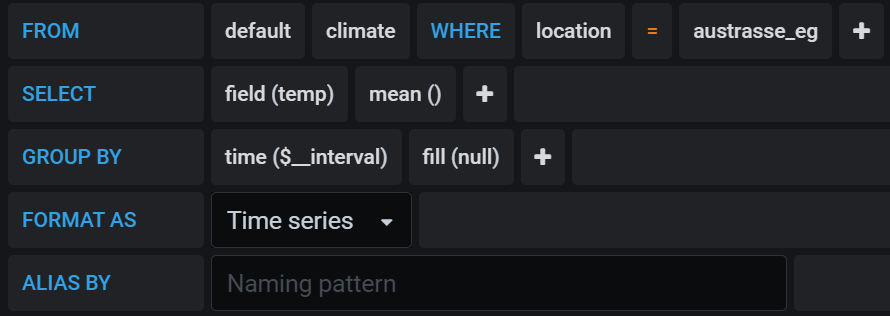
\includegraphics[width=0.85\textwidth]{./images/grafana-sql.png}  
    \end{center}
  \vspace{-5pt}
  \caption[Grafana Query]{Grafana Query}
  \label{fig:grafana-sql}
  \vspace{-10pt}
\end{figure}

Mit Grafana können Visualisierungen durch eine SQL-ähnliche Syntax einfach erstellt werden. Diese Syntax muss jedoch nicht selbst geschrieben werden, sondern kann über einen Wizard zusammengeklickt werden, wie in Abbildung \ref{fig:grafana-sql} erkannt werden kann \Zitat{GrafanaLabs.2020}.

\subsection{Umsetzung}
\label{sec:Prot:umsetzung2}

Im zweiten Prototypen wurde bei der Umsetzung mit der Datenverwaltung und \mbox{-visualisierung} begonnen. Da alle im Prototyp genutzten Komponenten in Docker Containern laufen sollten, jedoch das Orchestrieren einer derart hohen Zahl an Containern sehr aufwendig ist, wurde direkt von Beginn an Docker Compose genutzt, um diesem Problem entgegenzuwirken. Durch die Nutzung von Docker konnte das System lokal im gleichen Environment wie in der Deployment-VM entwickelt und getestet werden. Zu diesem Zeitpunkt war es geplant, den TIG-Stack, bestehend aus \Fachbegriff{Telegraf}, \Fachbegriff{InfluxDB} und \Fachbegriff{Grafana}, für die Datenverwaltung zu nutzen. Telegraf ist hierbei ein Server Agent, der Daten aktiv aus einer Menge von Quellen in eine andere Menge von Zielen schiebt. 

\begin{figure}[H]
  \vspace{10pt}
  \begin{center}
    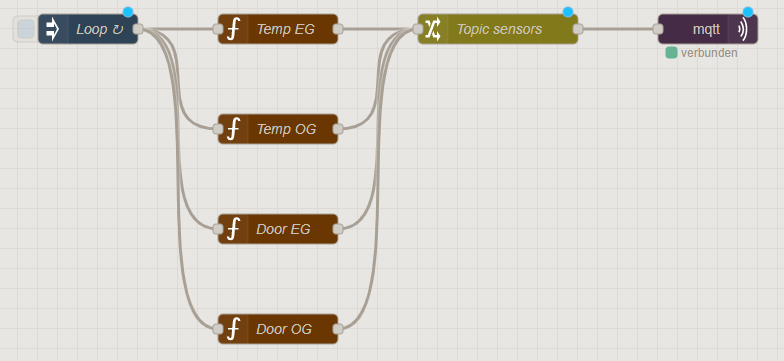
\includegraphics[width=0.75\textwidth]{./images/nodered.png}  
    \end{center}
  \vspace{-5pt}
  \caption[Simulation mit einem NodeRED Flow]{Simulation mit einem NodeRED Flow}
  \label{fig:nodered}
  \vspace{-10pt}
\end{figure}

Um den LoRaWAN-Teil des Prototypen zu simulieren, wurde das grafische Entwicklungswerkzeug \Fachbegriff{NodeRED} genutzt, mit dem in Sekundenschnelle Sensoren, die ihre Daten an einen MQTT Broker senden, durch JavaScript-Funktionen mit Zufallszahlen simuliert werden können. Mithilfe grafischer Bauteile können in NodeRED sogenannte Flows zusammengebaut werden, wie Abbildung \ref{fig:nodered} entnommen werden kann. Der Flow in der Abbildung simuliert zwei Temperatur- und zwei Türsensoren. Nachdem das Tool \Fachbegriff{Telegraf} so konfiguriert wurde, dass Daten aus dem MQTT Broker entnommen und in die InfluxDB geschrieben werden, konnten bereits erste Visualisierungen in Grafana erstellt werden. 

\begin{figure}[H]
  \vspace{10pt}
  \begin{center}
    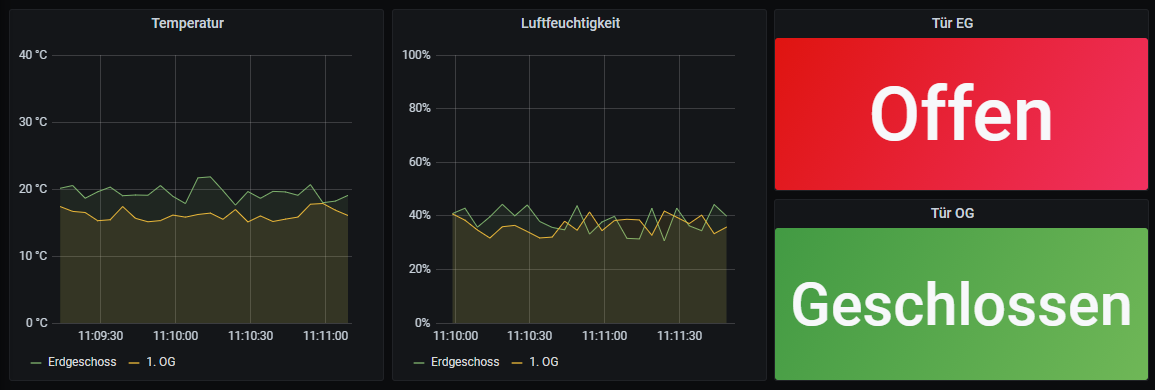
\includegraphics[width=1\textwidth]{./images/simple-dashboard.png}  
    \end{center}
  \vspace{-5pt}
  \caption[Dashboard Simulation]{Dashboard Simulation}
  \label{fig:dashboard-sim}
  \vspace{-10pt}
\end{figure}

In Abbildung \ref{fig:dashboard-sim} ist eine der unzähligen Möglichkeiten zur Datenvisualisierung in Grafana zu sehen. Die dargestellten Daten werden hierbei mit NodeRED zufällig generiert. Zu diesem Zeitpunkt waren fünf Docker Container im Einsatz: Eclipse Mosquitto als MQTT Broker, Telegraf als Data Server Agent, NodeRED zur Simulation des LoRaWAN-Netzes, InfluxDB als Datenbank und Grafana zur Visualisierung.

Nachdem die Speicherung und Visualisierung der Testdaten konfiguriert war, konnte der LoRaWAN-Teil des Prototypen bearbeitet werden. Da alle Komponenten des ChirpStack wie auch alle bisherigen Komponenten in Docker Containern bereitgestellt werden können, wurde so auch auch bei den ChirpStack-Komponenten vorgegangen. Hierfür wurde die offizielle Docker-Compose Vorlage für den ChirpStack\footnote{\url{chirpstack.io/project/guides/docker-compose/}} als Docker-Compose-Deployment genutzt. Da ein Großteil der Konfiguration durch die Vorlage wegfällt, konnte der ChirpStack in Sekundenschnelle gestartet werden. Im ChirpStack Application Server mussten nun neben kleinen Konfigurationsarbeiten, wie der Angabe der IP-Adresse des Network Servers und der Erstellung von Nutzern und deren Rechten, die Geräte, beginnend mit den Gateways, registriert werden. Besonders interessant ist hierbei die sehr ausgereifte Nutzer- und Organisationsverwaltung. Verschiedene Netzwerkbetreiber können sich Gateways teilen und somit ein gemeinsames Netzwerk aufbauen, ohne Zugriff auf die Daten des jeweils anderen zu haben.\\
Dass der ChirpStack richtig aufgesetzt war, konnte mit dem ChirpStack Simulator\footnote{\url{github.com/brocaar/chirpstack-simulator}}, einem Open-Source-Testprogramm für den ChirpStack, getestet werden. Nun konnte die Hardware ins System aufgenommen werden. Das verwendete Gateway verfügte jedoch über keinen freien Speicherplatz, weswegen die Gateway Bridge nicht direkt auf dem Gateway installiert werden konnte, sondern in der Azure VM bereitgestellt werden musste. In der Konfigurationssoftware des Gateways musste nun lediglich die IP-Adresse der Instanz der ChirpStack Gateway Bridge als Ziel für den UDP Packet Forwarder angegeben werden, um die Einrichtung des Gateways abzuschließen. Um die Endgeräte zu registrieren, konnten nun ähnlich wie beim The Things Network in Kapitel \ref{sec:Prot:umsetzung1} Applikationen erstellt werden, die eine Art Container für zusammengehörige Geräte darstellen. Ein elementarer Unterschied fiel im Vergleich zum ersten Prototypen auf: Decoder-Funktionen sind im ChirpStack nicht an die Applikation, sondern an sogenannte Device-Templates gebunden, welche dann wiederum verschiedenen Endgeräten zugeteilt werden. Somit können Geräte mit verschiedenen Datenstrukturen, die jedoch einen ähnlichen Zweck wie beispielsweise Temperaturmessung verfolgen, mit einer Applikation abgedeckt werden. Nachdem für die beiden Sensortypen Device-Templates erstellt waren und die Geräte selbst registriert waren, konnten bereits LoRaWAN-Pakete empfangen werden. 

\begin{figure}[H]
  \vspace{10pt}
  \begin{center}
    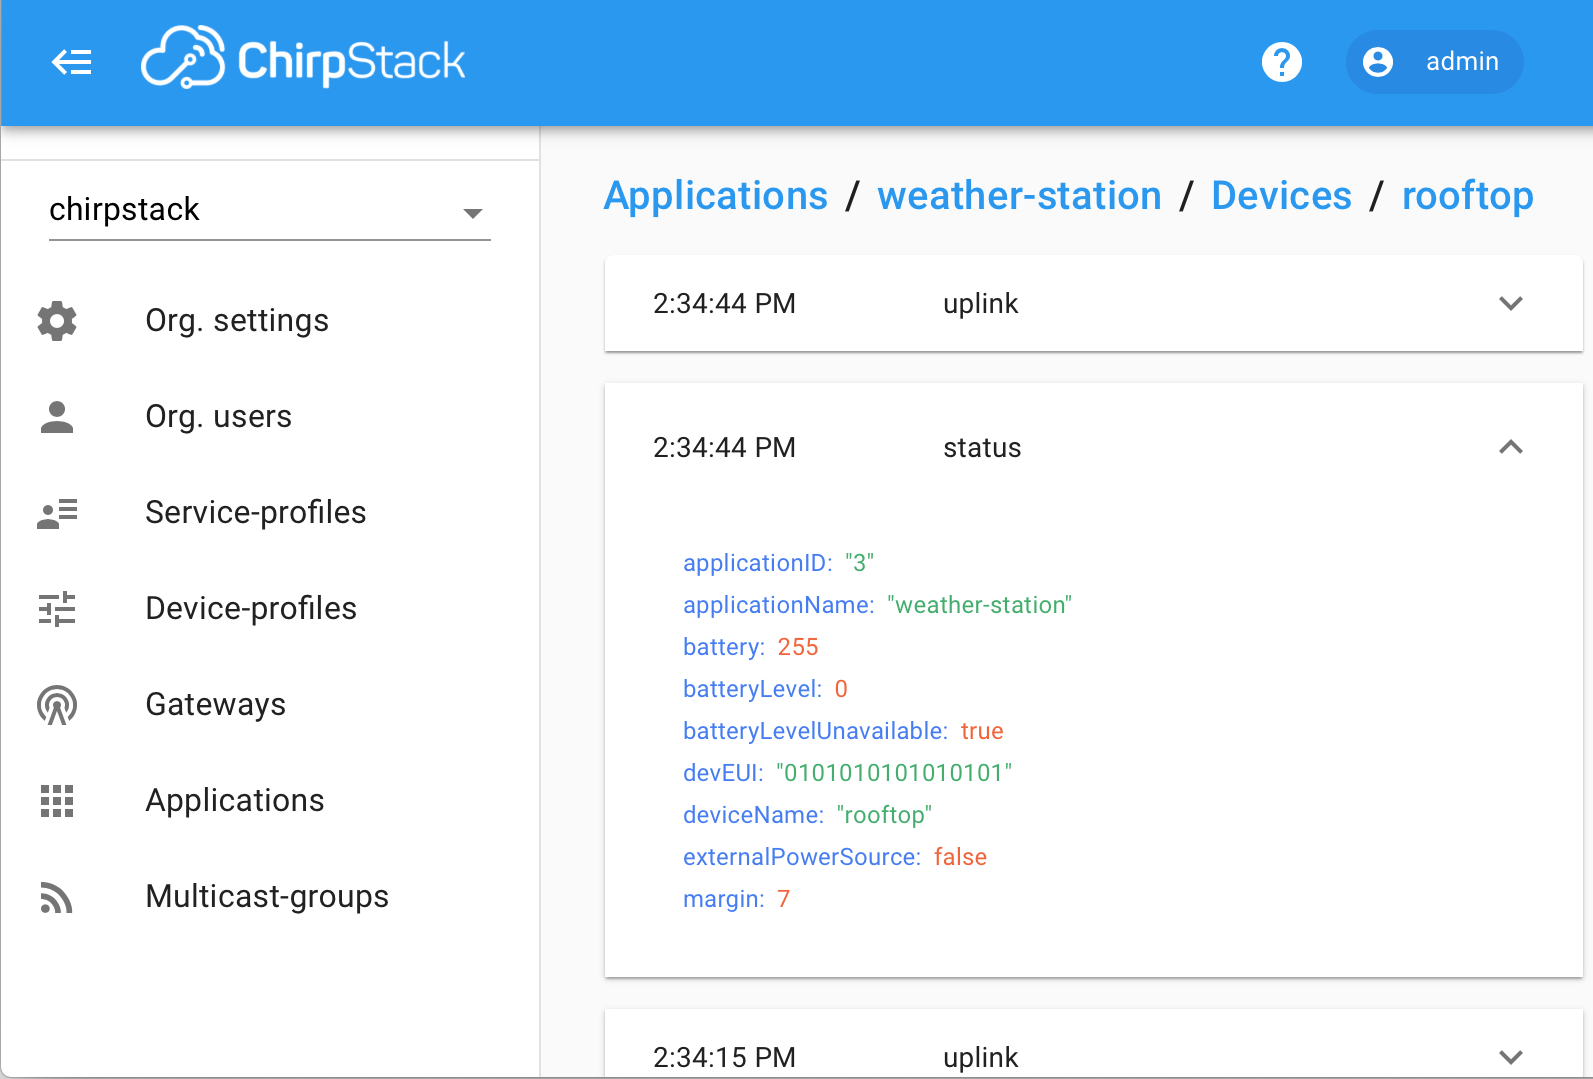
\includegraphics[width=0.9\textwidth]{./images/chirpstack-ui.png}
  \end{center}
  \vspace{-5pt}
  \caption[ChirpStack Benutzeroberfläche]{ChirpStack Benutzeroberfläche}
  \caption*{Quelle: {chirpstack.io/application-server (bearbeitet)}}
  \label{fig:chirpstack-ui}
  \vspace{-10pt}
\end{figure}

Abbildung \ref{fig:chirpstack-ui} zeigt ein Beispiel, wie der Datenempfang eines registrierten und konfigurierten Sensors in der Benutzeroberfläche des ChirpStack Application Servers aussehen könnte. 

Nun war es an der Zeit, den LoRaWAN-Teil des Prototypen mit der Datenverwaltung, in der bisher nur Testdaten gespeichert wurden, zu verbinden. Der erste Versuch fand hierfür mit der InfluxDB-Integration des ChirpStack Application Server statt. Durch die Angabe des HTTP-Write-Endpoints und der Authentifizierungsparameter der InfluxDB konnte die Integration schnell umgesetzt werden. Die Daten von empfangenen LoRaWAN-Paketen wurden nun erfolgreich in die Time-Series-Datenbank geschrieben. Bei der genaueren Betrachtung der gespeicherten Daten fiel jedoch schnell ein großes Problem auf: die InfluxDB-Integration speichert jeden Point (siehe Kapitel \ref{sec:Prot:systemkomponenten2:influx}) mit dem Namen des sendenden Endgeräts und dem Präfix \mbox{``device\_frmpayload\_data''} als Measurementnamen. Da es in der InfluxDB-Integration zum aktuellen Stand nicht möglich ist, eine eigene Datenstruktur zu verwenden, ist man an diese Benennung gebunden. Das Problem: da Points nun mit dem Gerätenamen als Measurement gespeichert werden, verfällt die Gruppierung von Geräten in Applikationen und resultiert in einer schnell sehr unübersichtlich werdenden Datenstruktur. Auch der Versuch den Server Agent \Fachbegriff{Telegraf} mit der MQTT-API, über die der ChirpStack empfangene Daten standardmäßig verbreitet, zu diesem Zweck zu nutzen, führte zum gleichen Problem. Aus diesen Gründen wurde für genau diesen Zweck der bereits erwähnte MQTT Consumer in der Programmiersprache Go entwickelt, dessen Funktionsprinzip bereits in Kapitel \ref{sec:Prot:systemkomponenten2:mqttcons} erläutert wurde. Die Komponente ähnelt also Telegraf stark, wobei der Schritt der Umwandlung des Datenformats hinzukommt. Auch diese Komponente wurde als \mbox{Docker} Container mit ins System aufgenommen und konnte leicht integriert werden. Versucht man nun beispielsweise einen speziellen Temperatursensor zu finden, ist es nicht nötig, alle Geräte zu durchsuchen, da zuerst nach dem Applikationstypen, welcher in der Datenbank das Measurement darstellt, gefiltert werden kann.\\
Somit war nun die Datenstruktur deutlich sinnvoller aufgebaut als die Datenstruktur der Integrations zum aktuellen Entwicklungsstand. Das System stand soweit fest und konnte nun auf das Production-System, im Fall dieses Prototypen eine Microsoft Azure VM, geladen werden. Auf dieser VM musste lediglich die Docker-Compose-Konfigurationsdatei genutzt werden, um das gleiche System wie im lokalen Environment herzustellen. Außerdem mussten Ports wie 1883 für MQTT und 80 für HTTP freigegeben werden, um die VM von außen erreichbar zu machen. Um das Gateway ins System aufzunehmen musste lediglich die IP-Adresse der Gateway Bridge in der Gatewaykonfiguration angepasst werden und das System lief vollständig im Production-System.

\begin{figure}[H]
  \begin{center}
    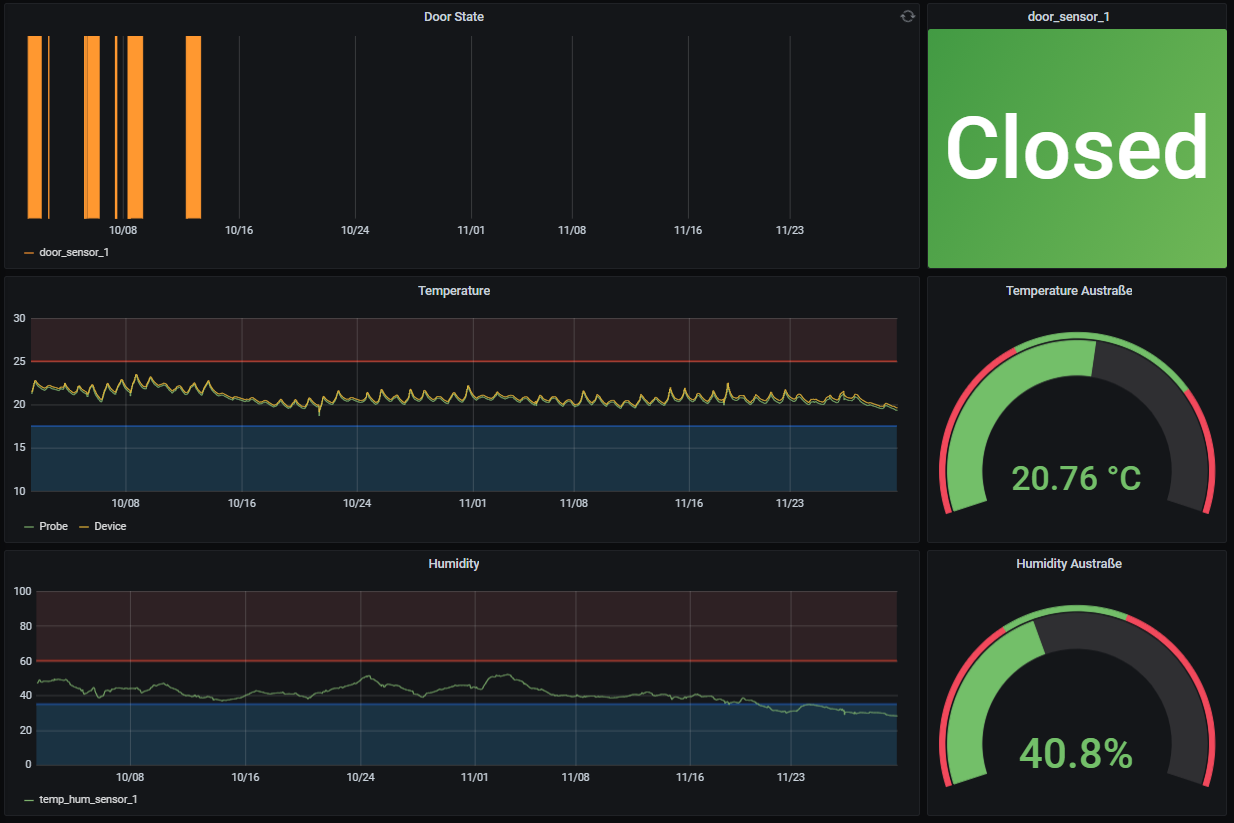
\includegraphics[width=1\textwidth]{./images/dashboard-longterm.png}  
    \end{center}
  \vspace{-5pt}
  \caption[IoT Dashboard: 2 Monate]{IoT Dashboard: 2 Monate}
  \label{fig:dashboard-longterm}
  \vspace{-5pt}
\end{figure}

Mit Grafana konnten nun anschauliche Dashboards über reale IoT-Daten erstellt werden. Abbildung \ref{fig:dashboard-longterm} zeigt das finale IoT-Dashboard und visualisiert die Temperatur und die Luftfeuchtigkeit eines Raumes sowie den Öffnungszustand einer Tür über jeweils einen Zeitraum von zwei Monaten.


\subsection{Architekturübersicht}
\label{sec:Prot:architektur2}

Gerade beim zweiten Prototypen ist es aufgrund der erhöhten Komplexität durch die hohe Anzahl an selbstverwalteten Services sinnvoll, sich einen Überblick über die Netzwerkarchitektur zu verschaffen. 

\begin{figure}[H]
  \vspace{10pt}
  \begin{center}
    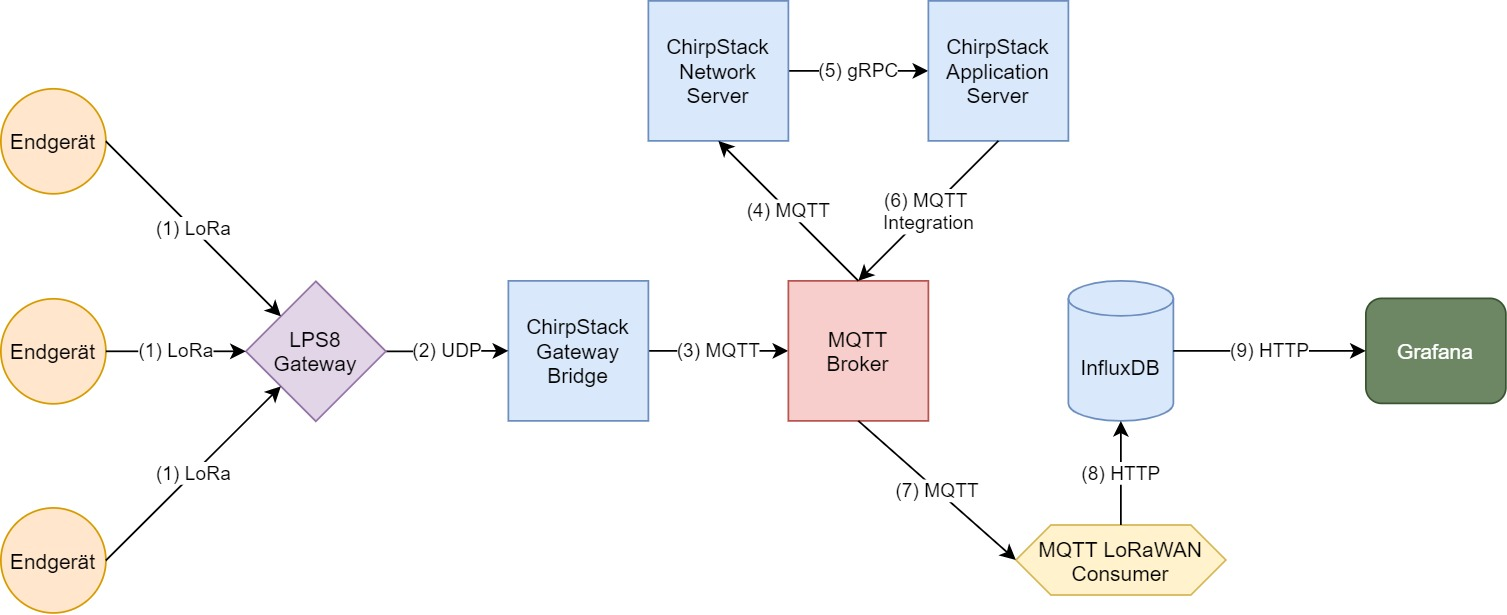
\includegraphics[width=1\textwidth]{./images/chirpstack_prototyp_architecture.jpg}
  \end{center}
  \vspace{-5pt}
  \caption[Prototyp 2: Architekturübersicht]{Prototyp 2: Architekturübersicht}
  \label{fig:chirpstack_prototype_architecture}
  \vspace{-10pt}
\end{figure}

In Abbildung \ref{fig:chirpstack_prototype_architecture} wird der Weg einer Nachricht vom LoRa-Endgerät bis zur Visualisierung in Grafana dargestellt. Nachdem das Gateway eine LoRaWAN-Nachricht von einem Endgerät empfangen hat, wird diese über das UDP Packet Forwarder Protocol an die Gateway Bridge weitergeleitet. Die Gateway Bridge legt diese Nachricht nun im MQTT Broker ab. Hätte das Gateway selbst eine Gateway Bridge installiert, könnte es die Nachricht direkt zum MQTT Broker senden. Der Network Server nimmt die Nachrichten als Subscriber vom MQTT Broker und verarbeitet diese weiter. Anders als beim The Things Network leitet dieser die verarbeiteten Nachrichten via gRPC direkt an den Application Server weiter und geht nicht erneut über den Message Broker. Die standardmäßig aktive MQTT Integration veröffentlicht nun die vom Application Server dekodierten Daten auf dem MQTT Broker. Die Daten verlassen nun den LoRaWAN-Stack, indem der selbst entwickelte MQTT Consumer diese vom Broker liest und über die HTTP-Schnittstelle in die InfluxDB schreibt. Grafana nutzt die Unterstützung für InfluxDB, um direkt aus der Datenbank Daten zur Visualisierung einzulesen. 

\subsection{Evaluation}
\label{sec:Prot:procontra2}

Auch die Evaluation des zweiten Prototypen beginnt mit einem Blick auf die Stärken des Systems, beginnend mit dem LoRaWAN-Teil. Mit dem ChirpStack kann ein eigenes LoRaWAN in kurzer Zeit instand gesetzt werden. Hierbei kann selbst entschieden werden, ob alle Softwarekomponenten online, verteilt oder gar vollständig offline in einem Intranet bereitgestellt werden sollen. Für sehr große Netzwerke besteht hier die Möglichkeit, das System nicht nur vertikal, sondern auch horizontal zu skalieren, indem Komponenten mehrfach gestartet werden, um die Systemlast pro Komponente zu senken. Wird ein LoRaWAN-Netzwerk mit dem ChirpStack aufgesetzt, ist dieses Netzwerk stets ein komplett privates Netzwerk. Dies birgt den Vorteil, dass lediglich die in Kapitel \ref{sec:ThHi:technisch} erwähnten lokalen LoRaWAN-Regulierungen, also der Duty Cycle, eingehalten werden müssen. Auf Netzwerkregulierungen wie eine maximale Uplinkzeit oder eine festgelegte Anzahl von Downlinknachrichten pro Tag beim The Things Network muss hier nicht geachtet werden. Somit ist es in einem privaten Netzwerk möglich, eine deutlich höhere Anzahl an Nachrichten zu senden.\\
Weiter bietet der ChirpStack eine durchdachte Nutzerverwaltung. Neben Nutzer- und Zugriffsrechten können beispielsweise Organisationen erstellt werden, die im Netzwerk koexistieren können, ohne die Daten des anderen zu sehen. So können Nutzergruppen wie beispielsweise verschiedene Abteilungen eines Unternehmens voneinander separiert werden, ohne dafür ein weiteres Netzwerk aufbauen zu müssen. Bei der Planung war die Erwartung, dass das Aufsetzen des Gateway im Netzwerk deutlich aufwendiger ist als beim The Things Network, da dort stets mit der Einfachheit durch den Verkauf eigener, vorkonfigurierter Gateways geworben wird. In der Umsetzung stellte sich dies jedoch als ähnlich einfach heraus und verursachte keinerlei Probleme. Auch das Hinzufügen neuer Endgeräte ähnelt dem The Things Network und funktionierte stets mühelos.\\
Hierbei fiel schnell ein kleiner Aspekt auf, der jedoch einen der größten Vorteile des ChirpStacks darstellt. Durch Device Templates können verschiedene Endgeräte mit unterschiedlichen Datenstrukturen in einer Applikation gruppiert werden, da nun Decoder-Funktionen nicht mehr pro Applikation sondern pro Device Template erstellt werden können. Somit ist es im ChirpStack beispielsweise möglich, Temperatursensoren von verschiedenen Herstellern in der gleichen Applikation zu verwalten, wodurch eine deutlich sinnvollere Datenstruktur entsteht. Auch die standardmäßig aktive MQTT-API für den externen Zugriff auf LoRaWAN-Daten bietet Vorteile gegenüber der des The Things Network. Während es nämlich im TTN nötig war, pro Applikation eigene Credentials für den Datenzugriff zu nutzen und somit pro Applikation eine eigene MQTT-Verbindung aufbauen zu müssen, reicht im ChirpStack eine einzige Verbindung aus. Ist ein MQTT-Client mit dem ChirpStack verbunden, kann er durch das Nutzen von Wildcards eine Subscription für alle Applikationen starten. Allgemein ist der ChirpStack außerdem sehr ausführlich dokumentiert und verfügt über eine große und hilfsbereite Community.\\
Auch die beiden Komponenten in der Datenverwaltung weisen einige Vorteile auf. Die InfluxDB ist eine äußert einfach nutzbare Datenbank. Die Inbetriebnahme ist durch die Nutzung von Docker sehr unkompliziert und erfordert kaum Konfiguration. Die Datenbank benötigt nur sehr geringe Systemressourcen und ist durch Retention Policies deutlich effizienter im Umgang mit Festplattenspeicher als typische relationale Datenbanken. Für große Szenarien existieren hier außerdem verteilte Deployments oder gar Cloudlösungen. Das Highlight des Prototypen ist das Visualisierungstool Grafana. Neben der InfluxDB kann Grafana aus unzähligen Datenquellen selbst gleichzeitig Daten anfordern und anschließend visualisieren oder regelbasiert auf Daten durch den Versand von E-Mails oder viele weitere Kanäle reagieren. Die Visualisierungsmöglichkeiten sind hierbei beinahe endlos. Selbst komplexe Queries an die Datenbank können mit einer SQL-ähnlichen Syntax zusammengeklickt werden und einfach dargestellt werden. Reichen die existierenden Features nicht aus, kann Grafana durch eine Vielzahl an Plugins erweitert werden. Da alle Komponenten typischerweise in Docker Containern gestartet werden, kann das System einerseits einfach lokal getestet, aber andererseits auch unkompliziert auf ein Production-System geladen werden. Durch die eigene Serververwaltung steht dem Netzbetreiber der Zugriff auf Logs und somit die Möglichkeit zur Fehlersuche und -behebung zur Verfügung. Außerdem kann das System durch das vorsichtige Freischalten von Ports zur Außenwelt von einem Großteil möglicher Angriffe geschützt werden. Im hier aufgesetzten Prototypen kann auf den ChirpStack Application Server beispielsweise nur aus dem eigenen Netzwerk zugegriffen werden. Letztendlich kann als Vorteil notiert werden, dass alle Netzwerkkomponenten in der gleichen Umgebung, sowohl online als auch offline, bereitgestellt werden können und dadurch die gesamte Verwaltung anders als beim ersten Prototypen an einer zentralisierten Stelle stattfindet.

Auch der zweite Prototyp birgt Nachteile. Der wohl offensichtlichste und größte dieser Nachteile ist, dass für die Instandsetzung des Prototypen selbst Server aufgesetzt und verwaltet werden müssen. Auch Sicherheit spielt hier eine große Rolle, da man Server durch unvorsichtige Konfiguration einer großen Angriffsfläche aussetzt. Soll ein cloudbasiertes System aufgesetzt werden, werden nicht nur grundlegende Kenntnisse in Linux, Docker und Sicherheitskonfiguration, sondern auch Kenntnisse in einer Cloud-Plattform wie beispielsweise Microsoft Azure benötigt. Müssen, wie in dieser Arbeit, weitere Tools wie der eigene MQTT-Consumer selbst implementiert werden, sind außerdem Programmierkenntnisse vonnöten. \newpage
Hand in Hand mit der eigenen Serveraufsetzung geht ein weiterer großer Nachteil dieses Prototypen: das System benötigt eine eigene Backupstrategie. Mit der hier gezeigten Architektur speichert das System jegliche Daten im Dateisystem. Gehen diese Daten verloren, gibt es ohne eine Backuplösung keine Möglichkeit, die verlorenen Daten wiederherzustellen. Neben klassischen Strategien wie dem direkten Speichern von Snapshots im Filesystem ist hier die einfachste Lösung, eine cloudbasierte und extern verwaltete InfluxDB-Instanz statt einer selbst bereitgestellten Instanz zu nutzen. Ein weiterer klarer Nachteil bezieht sich auf das LoRaWAN-Netzwerk selbst. Da das Netzwerk vollständig privat ist, muss die gesamte Abdeckung des zu unterstützenden Gebietes selbst mit eigenen Gateways aufgebaut werden. Gerade für mobile Endgeräte oder Szenarien, in denen Geräte in verschiedenen Regionen platziert sind, ist also die Nutzung des The Things Network und die damit verbundene existierende Netzabdeckung eine bessere Lösung. Auch in kleinen Projekten macht sich dies bemerkbar. Um LoRaWAN-Endgeräte nutzen zu können, muss bei diesem Prototypen zwingend ein eigenes Gateway in Betrieb genommen werden, was die Kosten deutlich vergrößert, während im The Things Network durch die existierende Abdeckung oft nicht zwangsweise ein eigenes Gateway aufgesetzt werden muss. Da fremde Gateways im TTN jedoch stets unerwartet vom Netz genommen werden können, sollte in Szenarien, in denen die Netzwerkstabilität essentiell wichtig ist, jedoch immer ein eigenes Gateway in Betrieb genommen werden. Dies gilt für beide Prototypen und ist somit nicht als Nachteil eines eigenen LoRaWAN-Netzwerks zu werten.\\ 
Ein Feature, welches sich im ersten Prototypen als sehr nützlich erwiesen hat, fehlt im zweiten Prototypen: das semantische Datenmapping. Daten werden hier in einer selbst definierten Struktur in eine Datenbank gespeichert und müssen stets vom Nutzer interpretiert werden. Somit ist die Nutzung der Anwendung für Personen, die die Datenstruktur nicht genau kennen, schwieriger als beim ersten Prototypen. Abschließend muss der Nachteil erwähnt werden, dass es beim zweiten Prototypen an einer Anbindung an ein Netz aus Services wie beim ersten Prototypen an Microsoft mangelt. So müssen hier Funktionen die auf externe Services zugreifen wie beispielsweise E-Mail-Alerts selbst konfiguriert werden, da das Tool selbst an keinen E-Mail-Server angebunden ist. Allgemein ist der zweite Prototyp also sehr gut in der Visualisierung der Daten, muss jedoch um einigen Features des ersten Prototypen nachzukommen, um weitere Konfiguration oder gar neue Softwarekomponenten erweitert werden.


\clearpage

\chapter{Fazit}
\label{cha:fazit}

In dieser Bachelorarbeit wurde das Funkprotokoll LoRa ausführlich analysiert und anhand von praxisorientierten Tests in Form von zwei verschiedenen Prototypen auf die Eignung für Smart Building IoT-Services geprüft.

\section{LoRa im Vergleich}

Um das Protokoll LoRa besser einordnen zu können, wurden zu Beginn typisch verwendete IoT-Protokolle betrachtet. Es fiel schnell auf, dass die bisher meist verwendeten Wireless Private Area Network (WPAN) Techniken wie Zigbee und Bluetooth Low Energy zwar weiterhin sehr beliebt bleiben, jedoch große Schwächen für IoT-Lösungen aufzeigen. Eine dieser Schwächen ist, dass die Protokolle meist nicht energieeffizient genug arbeiten, um Endgeräte über größere Zeiträume mit Batterien betreiben zu können. Außerdem sind die maximalen Sendereichweiten von etwa 100 Metern für viele Szenarien nicht ausreichend, besonders da die Reichweite durch Hindernisse wie beispielsweise Wände stark verringert wird. Darüber hinaus wurde festgestellt, dass WPAN-Techniken für sehr hohe Geräteanzahlen eher ungeeignet sind. Es sind jedoch auch klare Vorteile der betrachteten Techniken aufgefallen. Protokolle wie Zigbee und BLE überzeugen durch Einfachheit sowohl bei der Nutzung als auch in den Netzwerkstrukturen selbst. Außerdem senden die Protokolle mit verhältnismäßig hohen Bandbreiten und geringen Latenzen, weswegen die Protokolle auch für die Datenübertragung in Echtzeit geeignet sind.

Nach den WPAN-Techniken wurden in der Arbeit Low Power Wide Area Network (LPWAN) Techniken behandelt. Techniken dieser Klasse haben in den vergangen Jahren gerade im IoT-Bereich immens an Beliebtheit gewonnen und lösen viele Probleme, die traditionelle IoT-Protokolle aufweisen. Mit LPWAN-Techniken ist es möglich, Daten über große Distanzen mit sehr geringem Energieaufwand zu versenden. Netzwerke sind sehr flexibel und skalierbar, wobei bereits einige Netzwerke große Teile der Erde abdecken. Die beiden Protokolle Sigfox und NB-IoT gehören zur Klasse der LPWAN-Techniken und wurden in der Arbeit präziser betrachtet. So baut NB-IoT auf das bereits existierende Mobilfunknetz auf und weist dadurch eine große Netzwerkabdeckung vor. Der größte Vorteil des Protokolls ist die sehr reife Infrastruktur, die zum Mobilfunk gehört. So ist beispielsweise Datensicherheit oder Skalierbarkeit des Netzes bereits vorhanden. Auch die hohe Energieeffizienz spricht für NB-IoT. Da das Protokoll im lizenzierten Spektrum operiert, ist die Nutzung des Netzes jedoch mit vergleichsweise hohen Kosten verbunden. Außerdem ist es Nutzern nicht möglich, eigene Netze zu erstellen, wodurch eine große Abhängigkeit entsteht. Sigfox bietet ebenfalls ein bereits existierendes Netzwerk an und verfolgt das Ziel, ein globales Netzwerk aufzubauen. Zur Nutzung des Sigfox-Netzwerks gehört die Sigfox-Cloud, in die Daten von Endgeräten über Empfangsstationen weitergeleitet und gespeichert werden. Sigfox überzeugt durch ein Gesamtpaket von preiswerten Geräten, einer großen Netzwerkabdeckung und einem kompletten Device-To-Cloud Datenversand. Jedoch ist auch die Nutzung von Sigfox mit Problemen verbunden. Wie auch bei NB-IoT ist es nicht möglich, eigene Netzwerke zu erstellen, was gerade dann problematisch ist, wenn die Zielregion nicht durch das Sigfoxnetzwerk abgedeckt ist. Da Sigfox im frei nutzbaren und unlizenzierten Spektrum arbeitet, sind zwar die Kosten gering, jedoch wird das Sendeverhalten im Netzwerk stark eingeschränkt. Mit Sigfox kann ein Gerät lediglich 140 Nachrichten am Tag senden, wodurch Szenarien, in denen das Senden von Echtzeitdaten oder eine zuverlässige Berichterstattung erforderlich sind, mit Sigfox nicht realisiert werden können.

LoRa und das damit verbundene Protokoll zählt zu den LPWAN-Techniken und ist von den erwähnten Protokollen am ehesten mit Sigfox in Verbindung zu bringen. So ist auch LoRa ein Protokoll, mit welchem Daten über große Distanzen mit geringem Energieverbrauch gesendet werden können. Das Protokoll ist außerdem sehr robust gegen Interferenzen und weitere typische Funkprobleme. Wie auch Sigfox operiert LoRa im unlizenzierten Spektrum und kann somit frei genutzt werden. Normalerweise muss man sich bei der Nutzung des Spektrums lediglich an den sogenannten Duty Cycle halten. Dieser reguliert die erlaubte Sendezeit auf einen festgelegten Prozentsatz eines Zeitfensters. Dieser Wert variiert jedoch je nach Region, wobei der Duty Cycle für LoRa in Deutschland bei 1\%, also beispielsweise 36 Sekunden pro Stunde liegt. Bei externen Netzanbietern gibt es jedoch meist noch weitere Regulierungen. Für typische IoT-Szenarien, in denen wenige und vor allem kleine Datenpakete versendet werden, ist dies aber in der Regel kein Problem.\\ 
Während das proprietäre Protokoll LoRa lediglich die erste Schicht des TCP/IP-Schichtenmodells abdeckt, ist das Open-Source-Protokoll LoRaWAN für die darüber liegenden Schichten zuständig und definiert außerdem die Struktur des Netzwerks. Typische LoRaWAN-Netzwerke sind in die verschiedenen Komponenten Packet Forwarder, Gateway Bridge, Join Server, Network Server und Application Server aufgeteilt, wobei der Network Server den Kern des Netzwerks und somit den Stern der Sterntopologie darstellt. Zwar existieren hierfür viele externe Netzwerkanbieter, es ist jedoch, anders als bei Sigfox und NB-IoT, möglich, eigene Netzwerke aufzubauen. Wie auch beim Protokoll Sigfox erreicht man durch einen LoRaWAN-Stack eine Device-To-Cloud-Connectivity. Auch Sicherheit ist bei LoRaWAN ein großes Thema. Die Sicherheit von LoRaWAN basiert auf einer AES-Verschlüsselung und einem System aus verschiedenen Keys, sodass selbst Komponenten im Netzwerk nur den für sie relevanten Teil einer Nachricht sehen können. Als Abschluss des theoretischen Hintergrunds wurden neben einer kurzen Beschreibung des \mbox{Messaging} Protokolls MQTT das The Things Network und das Unternehmen The Things Industries vorgestellt. Beim The Things Network handelt es sich um ein globales, öffentliches LoRaWAN-Netzwerk, wobei jeder freien Zugriff auf alle teilnehmenden Empfangsstationen erhält und auch eigene Stationen ans Netzwerk anbinden kann. The Things Industries bietet neben Consulting und fertigen LoRaWAN-Lösungen für das The Things Network außerdem vorkonfigurierte LoRaWAN-Geräte an, um Kunden den Einstieg zu erleichtern.

\section{Netzwerkarchitekturen für IoT mit LoRa}

Im weiteren Verlauf der Arbeit wurden zwei verschiedene LoRaWAN-Netzwerk-Prototypen behandelt. Mithilfe dieser Prototypen sollte erforscht werden, welche der unzähligen Auswahlmöglichkeiten an Softwarekomponenten für welche Szenarien geeignet sind. Als Endgeräte wurden hierfür jeweils ein Temperatur- und Luftfeuchtigkeitssensor und ein Türsensor verwendet. Außerdem wurde dargestellt, warum für die Speicherung von IoT-Daten Time-Series-Datenbanken mit am besten geeignet sind. 

Beim ersten Prototypen war die Nutzung möglichst vieler, bereits existierender, Hardware- und Softwarekomponenten das Ziel. Die Erwartungen an den Prototypen waren hierbei vor allem ein schnelles und einfaches Setup des Netzwerks mit wenig Konfigurationsaufwand, gute Skalierbarkeit und die Möglichkeit, eingehende Daten zu visualisieren und auf diese in Echtzeit zu reagieren. Die Kernkomponenten des Prototypen waren hierbei im LoRaWAN-Teil das The Things Network und im Datenverwaltungsteil Microsofts Azure IoT Central. Wie bereits erwartet, war das Hinzufügen der Endgeräte ins LoRaWAN-Netzwerk sehr einfach, da keine Server oder gar Services aufgesetzt werden mussten. Da der Arbeitsplatz, an dem der Prototyp aufgebaut wurde, bereits durch ein fremdes LoRaWAN-Gateway abgedeckt war, wäre beim Aufbau kein eigenes Gateway nötig gewesen. Hierdurch wären Hardwarekosten des Systems deutlich geringer ausgefallen. Da jedoch bei der Nutzung keine Garantie bestand, dass fremde Gateways konstant erreichbar sein würden, wurde sicherheitshalber trotzdem ein Gateway von The Things Industries in Betrieb genommen.\\
Auch das Aufsetzen einer Azure IoT Central Anwendung selbst verlief problemlos. Besonders positiv fiel hierbei die Möglichkeit auf, die Datenstruktur der verschiedenen Endgeräte in Form sogenannter Device Templates zu definieren, um ein semantisches Mapping eingehender Daten zu erhalten, was die Datennutzung sehr erleichtert. Als weitere Stärke fiel die Integration in die Microsoft-Infrastruktur auf. So können in einer Azure IoT Central Anwendung beispielsweise in kürzester Zeit \mbox{E-Mail}-Alerts beim Eintritt festgelegter Regeln konfiguriert werden, ohne dafür einen E-Mail-Server hinterlegen zu müssen. Auch die Integration der Nutzerverwaltung von Microsoft funktionierte hier tadellos. Weiter konnten nun beliebige \mbox{Microsoft} Softwarekomponenten wie beispielsweise eine Time-Series-Datenbank zur permanenten Speicherung eingehender Daten ins Netzwerk hinzugefügt werden.\\
Besonders schwierig war beim Aufbau des Prototypen die Verbindung zwischen dem The Things Network und der Azure IoT Central Anwendung. Hierfür wurde eine Azure Function, eine Art von HTTP-Endpoint, genutzt und in Microsoft Azure bereitgestellt. Per HTTP-Integration konnten Daten aus dem The Things Network nun über den HTTP-Endpoint in die IoT Central Anwendung weitergeleitet werden. Dies ist als Schwäche dieses Prototypen anzusehen, da dies unverhältnismäßig aufwändig für eine Verbindung des LoRaWAN-Netzes mit der Datenverwaltung ist. Außerdem sind grundlegende Programmierkenntnisse sowie fortgeschrittene Kenntnisse in einer Cloud-Plattform wie beispielsweise Microsoft Azure für diese Verbindung erforderlich. Allgemein überzeugte der Prototyp vor allem durch das einfache Setup der beiden Hauptkomponenten und die Nutzung des öffentlichen LoRaWAN-Netzwerks.

Beim Aufbau des zweiten Prototypen wurden ausschließlich Komponenten mit einer Open-Source-Lizenz genutzt und selbst in einer virtuellen Maschine in Microsoft Azure mithilfe von Docker aufgesetzt. Zu erwähnen gilt hierbei, dass dieser Prototyp auch vollständig offline bereitstellbar und mit allen Funktionen nutzbar ist. Die größte Erwartung an den Prototypen war hierbei ein großer Aufwand beim Aufsetzen der Softwarekomponenten und bei der Serverkonfiguration. Da das Unternehmen The Things Industries mit der einfachen Inbetriebnahme ihrer Geräte wirbt, wurde außerdem damit gerechnet, dass das Setup eines eigenen LoRaWAN-Netzwerks aufwendig sein würde. Auch waren Erwartungen an das System ein vollständiger Einblick in Protokolle aller genutzten Services und eine höhere Anzahl an sendbaren Nachrichten, da anders als beim The Things Network in einem eigenen LoRaWAN-Netzwerk neben dem Duty Cycle keine weiteren Regulierungen existieren.
Als LoRaWAN-Stack wurde für den zweiten Prototypen der Open-Source ChirpStack verwendet, welcher dem The Things Network in der Funktionsweise sehr stark ähnelt. Das Setup des LoRaWAN-Stacks war erstaunlich einfach, da alle Komponenten in Docker Containern bereitgestellt werden können und sogar fertige Docker-Compose-Konfigurationsdateien existieren, mit denen das bereits vorkonfigurierte System in kürzester Zeit in Betrieb genommen werden kann. Das Hinzufügen des LoRaWAN-Gateways war ebenfalls einfacher als erwartet. Hierzu musste lediglich die IP-Adresse und der Port der Gateway Bridge, einer der Komponenten des ChirpStack, in der Software des Gateways hinterlegt werden. Nun konnte das Gateway in der Konfigurationssoftware des ChirpStacks ins System aufgenommen werden. Anders als beim ersten Prototypen war dieses Netzwerk nun vollkommen privat und hatte neben den eigenen Gateways keine weitere Netzwerkabdeckung. Das Sendeverhalten war jedoch lediglich durch den Duty Cycle, nicht aber wie beim The Things Network durch eine Fair Use Policy, reguliert. Durch eine durchdachte Nutzer- und Rechteverwaltung konnten Nutzern Zugriffsrechte auf die einzelnen Komponenten des Netzwerks wie Gateways oder Endgeräte erteilt werden.

Zur Datenverwaltung und -speicherung wurden als Software\-komponenten ein selbst entwickelter MQTT-Consumer zum Auslesen der Daten aus dem ChirpStack, eine InfluxDB zur permantenten Datenspeicherung und Grafana zur Datenvisualisierung genutzt. Auch diese Komponenten wurden in Docker Containern bereitgestellt. Auch die Konfiguration der Komponenten stellte sich hier als überraschend einfach heraus. Im Vergleich zum ersten Prototypen waren für diesen Prototypen deutlich mehr Kenntnisse in der Softwareentwicklung, Azure und allgemeiner Serververwaltung nötig. Auch wichtige Elemente wie eine Backupstrategie oder Kommunikationskanäle für Alerts müssten mit diesem Prototypen selbst konfiguriert werden, während die externen Services beim ersten Prototypen viele dieser Arbeiten abnehmen. Beim zweiten Prototypen fielen allgemein die unzähligen Möglichkeiten zur Datenvisualisierung in Grafana, die vollständige Kontrolle über alle Softwarekomponenten und die Flexibilität durch die verteilte Netzwerkarchitektur sehr positiv auf.

\section{Zusammenfassung}

Zusammenfassend lässt sich sagen, dass das Protokoll LoRa für Zwecke wie Smart Buildings aber auch für Smart City Szenarien, die sich über größere Gebiete wie Städte oder Landkreise erstrecken, sehr gut eignet. Das Protokoll liefert verbunden mit LoRaWAN eine für IoT-Lösungen hervorragende Balance aus Sendereichweite, Bandbreite, Energieverbrauch und Kosten und liegt in einer Nische zwischen dem sehr ähnlichen, aber stark regulierten, Protokoll Sigfox und der auf den Mobilfunk basierenden Technik NB-IoT. LoRa und LoRaWAN überzeugen verglichen mit diesen Techniken durch die Flexibilität beim Netzwerkaufbau und einem nur wenig beschränkten Sendeverhalten der freien Nutzung des Funkspektrums. Während das Protokoll für typische IoT-Lösungen sehr gut geeignet ist, sollte in Usecases, in denen Echtzeitdaten oder eine sehr hohe Bandbreite erforderlich sind, eher zu klassischen PWAN-Techniken wie BLE oder Zigbee gegriffen werden. Sind die große Reichweite, aber auch eine hohe Nachrichtenanzahl unabdingbar, sollte eine mobilfunkbasierte Technik wie NB-IoT genutzt werden, wobei hier die Geräte- und Netzwerkkosten deutlich höher sind.

Die Frage, welche Netzwerkarchitektur am sinnvollsten genutzt werden sollte, hängt von den Anforderungen ans System ab. Das The Things Network als LoRaWAN-Netzwerk erlaubt den einfachsten Einstieg in das Thema LoRa. Das Netzwerk kann genutzt werden, ohne selbst Server oder Services aufsetzen zu müssen. Die Nutzung des öffentlichen Netzwerks spart nicht nur Kosten, sondern bietet Nutzern zukünftig die Möglichkeit, global LoRaWAN-Signale zu empfangen. Für große IoT-Netzwerke mit einem hohen Maß an Nachrichten kommt das The Things Network jedoch schnell an seine Grenzen. Zwar bietet The Things Industries eigene, maßgeschneiderte Deployments für große Netzwerke an, jedoch werden diese schnell sehr kostspielig. Die Prototypen erwecken daher den Eindruck, dass sich die Bereitstellung eines eigenen LoRaWAN-Stacks wie beispielsweise dem ChirpStack für große oder gar kommer\-zielle Netze besser eignet. Durch das Aufsetzen eines privaten Netzwerks fallen viele Regulierungen wie beispielsweise die Fair Access Policy im The Things Network weg und erlauben einen flexibleren Datenaustausch mit Endgeräten. Außerdem erhält der Nutzer volle Kontrolle über alle Netzwerkkomponenten und kann so Dinge wie die Verwaltung von Logs, Datenspeicherung oder verteilte Deployments selbst steuern. Außerdem können private Netzwerke offline oder in einem Intranet erstellt werden, während öffentliche Netzwerke stets einen Internetzugang benötigen. Die netzwerkinterne Kommunikation läuft aufgrund der Modularität der Softwarekomponenten typischerweise zum Großteil über Messaging Protokolle wie MQTT oder Remote Procedure Call Protokollen wie gRPC. Bei beiden LoRaWAN-Stacks gilt es allgemein nicht zu vergessen, dass beide Stacks noch täglich verbessert werden, und somit nicht anhand einzelner, fehlender Features wie mehreren Decoder-Funktionen pro Applikation im The Things Network bewertet werden sollten. 

Auf der Seite der Datenverwaltung und -visualisierung können ebenfalls beide Versionen sinnvoll eingesetzt werden. Azure IoT Central entpuppte sich besonders dann als sinnvoll, wenn das System von einer Integration in die Microsoft Infrastruktur profitiert. Die existierende Microsoft Nutzerverwaltung, das einfache Senden von Nachrichten über verschiedene Kommunikationskanäle wie E-Mail und das Hinzufügen unzähliger Microsoft-Services sprechen sehr für die IoT-Plattform. Jedoch ist mit der Nutzung von Azure IoT Central das Aufsetzen einer IoT Device Bridge verbunden, welche Daten zwischen dem LoRaWAN-Netzwerk und der IoT Central Anwendung austauscht. Auch die stark eingeschränkten Möglichkeiten zur Visualisierung eingehender Daten sind ein Nachteil von Azure IoT Central Anwendungen. Mit dem alternativen Open-Source-Stack bestehend aus einer InfluxDB als Datenbank und Grafana zur Datenvisualisierung erhält man eine einfach nutzbare Plattform zur Datenverwaltung. Besonders überzeugend ist hierbei Grafana mit seinen unzähligen Möglichkeiten zur Darstellung von Daten. Da jedoch in diesem Stack keine Anbindung an eine existierende Infrastruktur besteht, müssen Dinge wie eine Nutzerverwaltung oder Kommunikationskanäle für Alerts selbst aufgebaut werden. Stellt dies für den Nutzer kein Problem dar, so kann man anhand der in der Arbeit erstellten Prototypen schlussfolgern, dass der Open-Source-Stack auf Datenverwaltungsebene für die meisten Szenarien besser geeignet ist.

\section{Ausblick}

Da in dieser Arbeit allgemein nur wenig auf die Hardwareseite von LoRa eingegangen wurde, bietet sich hier ein großes Potenzial für weitere Forschungen. Neben der genauen Funktionsweise des Datentransports über LoRa oder des Aufbaus von LoRa-Geräten könnte es außerdem profitabel sein, Strukturen zur zuverlässigen Anbindung von IoT-Lösungen mit LoRa an ansteuerbare Hardware wie Klimaanlagen oder automatisierte Bewässerungsanlagen zu analysieren.
%\clearpage


% Literaturverzeichnis ---------------------------------------------------------
%   Das Literaturverzeichnis wird aus der BibTeX "bibliography.bib" erstellt.
% ------------------------------------------------------------------------------
\bibliography{bibliography} % Aufruf: bibtex Masterarbeit
\bibliographystyle{natdin} %DIN-Stil des Literaturverzeichnisses
%\bibliographystyle{myplainnat} % custom


Ich, \autor, Matrikel-Nr.\ \matrikelnr, versichere hiermit, dass ich die vorliegende Arbeit mit dem Thema
\begin{quote}
\textit{\titel\ - \untertitel}
\end{quote}
selbständig verfasst und keine anderen als die angegebenen Quellen und Hilfsmittel benutzt habe, wobei ich alle wörtlichen und sinngemäßen Zitate als solche gekennzeichnet habe. Die Arbeit wurde bisher keiner anderen Prüfungsbehörde vorgelegt und auch nicht veröffentlicht.\\

\ort, den \today
\vspace*{1cm}\\
\rule[-0.1cm]{5cm}{0.5pt}\\
\textsc{\autor} 
 % Eidesstattliche Erklärung

% Anhang -----------------------------------------------------------------------
%   Die Inhalte des Anhangs werden in der Datei "Anhang.tex" inkludiert.
% ------------------------------------------------------------------------------
\begin{appendix}
    \clearpage
    \pagenumbering{alph}
    \chapter{Anhang}
    \label{sec:Anhang}
    % Rand der Aufzählungen in Tabellen anpassen
    \setdefaultleftmargin{1em}{}{}{}{}{}
     \section{Inhalt des Datenträgers}
\label{apx:Datentraeger}

Der dieser Arbeit beigelegte Datenträger beinhaltet die folgenden Materialen.

\begin{description}
\item[\texttt{./azure_iot_central}] ~ \linebreak 
\noindent\hspace*{10mm} Azure IoT Device Templates und Architekturübersicht
\item[\texttt{./decoder_functions}] ~ \linebreak 
\noindent\hspace*{10mm} Decoder-Funktionen für die verwendeten Endgeräte
\item[\texttt{./full_deployment}] ~ \linebreak 
\noindent\hspace*{10mm} Gesamtes Deployment des zweiten (Open-Source-)Prototypen
\item[\texttt{./mqtt_lorawan_consumer}] ~ \linebreak 
\noindent\hspace*{10mm} Selbst entwickelter MQTT-Consumer für Chirpstack-API
\item[\texttt{./tig_testing}] ~ \linebreak 
\noindent\hspace*{10mm} Testprojekt für Grafana \& InfluxDB \& Telegraf mit NodeRED
\end{description}
\end{appendix}

% Index ------------------------------------------------------------------------
%   Zum Erstellen eines Index, die folgende Zeile auskommentieren.
% ------------------------------------------------------------------------------
%\printindex


\end{document}
